\documentclass{report}

%%%%%%%%%%%%%%%%%%%%%%%%%%%%%%%%%%%%%%%%%%%%%%%%
% This seciont would include all the required
% packages.
%%%%%%%%%%%%%%%%%%%%%%%%%%%%%%%%%%%%%%%%%%%%%%%%
% package to wrap text around figures.
\usepackage{wrapfig}

% for pseudo-code
\usepackage{algorithmic}

% for argmin and argmax
% https://tex.stackexchange.com/a/5255
\usepackage{amsmath}
\DeclareMathOperator*{\argmax}{arg\,max}
\DeclareMathOperator*{\argmin}{arg\,min}

% table of contents are in different lines.
\usepackage[utf8]{inputenc}

% for table's toprule and bottomrule
\usepackage{booktabs}

\usepackage{tikz}

% to include pdfpages
\usepackage{pdfpages}

% for table
\usepackage{multirow}

% code listing
\usepackage{tcolorbox}
\usepackage{listings}
\lstdefinestyle{mystyle}{
	backgroundcolor=\color{backcolour},   
	commentstyle=\color{codegreen},
	keywordstyle=\color{magenta},
	numberstyle=\tiny\color{codegray},
	stringstyle=\color{codepurple},
	basicstyle=\ttfamily\footnotesize,
	breakatwhitespace=false,         
	breaklines=true,                 
	captionpos=b,                    
	keepspaces=true,                 
	numbers=left,                    
	numbersep=5pt,                  
	showspaces=false,                
	showstringspaces=false,
	showtabs=false,                  
	tabsize=2
}
\lstset{style=mystyle}

% page dimensions
\usepackage{geometry}
\geometry{
	a4paper,
	total={170mm,257mm},
	left=20mm,
	top=20mm,
}

% captioned images or figures in LaTeX.
\usepackage{float}

% for referencing
\usepackage[%  
colorlinks=true,
pdfborder={0 0 0},
linkcolor=red
]{hyperref}

% to make caption bold.
% https://tex.stackexchange.com/a/32463/277097
\usepackage[labelfont=bf]{caption}

% increase spacing between paragraphs
\setlength{\parskip}{1mm}

% colorbox
% https://texdoc.org/serve/tcolorbox.pdf/0
\usepackage{tcolorbox}

% citations
\usepackage{cite}

% to left indent caption
% https://tex.stackexchange.com/a/275141
%\captionsetup{justification=justified,singlelinecheck=false}

%%%%%%%%%%%%%%%%%%%%%%%%%%%%%%%%%%%%%%%%%%%%%%%%
% package end.
%%%%%%%%%%%%%%%%%%%%%%%%%%%%%%%%%%%%%%%%%%%%%%%%

\title{
	Masterarbeit \\
	Robust Registration to a template brain  \\
	for the Drosophila larva \large }

\author{Harsha Yogeshappa}

% define RWTH Color
% https://www.color-hex.com/color-palette/33602
\definecolor{rwth-blue-1}{rgb}{0.00, 0.33, 0.62}
\definecolor{rwth-blue-2}{rgb}{0.25, 0.50, 0.71}
\definecolor{rwth-blue-3}{rgb}{0.55, 0.72, 0.89}
\definecolor{rwth-blue-4}{rgb}{0.78, 0.87, 0.95}
\definecolor{rwth-blue-5}{rgb}{0.90, 0.94, 0.98}
\definecolor{codegreen}{rgb}{0,0.6,0}
\definecolor{codegray}{rgb}{0.5,0.5,0.5}
\definecolor{codepurple}{rgb}{0.58,0,0.82}
\definecolor{backcolour}{rgb}{0.95,0.95,0.92}

% To change the color of chapter
% https://tex.stackexchange.com/a/75670
\usepackage{xcolor}
\usepackage{sectsty}
\chapterfont{\color{rwth-blue-1}}  % sets colour of chapters

% To change color of section headers.
\usepackage{titlesec}
\usepackage{color}

\titleformat{\section}
{\color{rwth-blue-1}\normalfont\Large\bfseries}
{\color{rwth-blue-1}\thesection}{1em}{}

\titleformat{\subsection}
{\color{rwth-blue-1}\normalfont\large\bfseries}
{\color{rwth-blue-1}\thesubsection}{1em}{}

\titleformat{\subsubsection}
{\color{rwth-blue-2}\normalfont\large\bfseries}
{\color{rwth-blue-2}\thesubsection}{1em}{}
% To change the color of caption
% \usepackage[font={color=rwth-blue-1},figurename=Figure]{caption}

\begin{document}
	\maketitle
	\newpage
	
	\hypersetup{linkcolor=rwth-blue-1}
	\tableofcontents
	\newpage
	
	\chapter{Introduction}
	The purpose of this chapter is to introduce the main focus of this thesis and provide an overview of its key components. Specifically, we will present the research question that drives our study, the background and motivation for this work, the specific objectives and hypotheses we are aiming to test, and the overall structure of the thesis. Our goal is to provide a clear and concise introduction to the content of the following chapters, giving the reader a clear roadmap for the rest of the document.
	
	% https://tex.stackexchange.com/a/8633/277097
	\section{Research question: Image Registration}
	Image registration is the process of aligning or registering two or more images so that they can be compared or combined. It is a fundamental technique in many fields, including medical imaging, computer vision, image processing, robotics, remote sensing, and computer graphics. Some examples of where image registration is used outside of medicine include:
	\begin{enumerate}
		\item \textbf{Computer vision}: Image registration is often used in computer vision to align images of the same scene or object, taken at different times or from different viewpoints, in order to facilitate image analysis and recognition tasks.
		\item \textbf{Image processing}: Image registration is used in image processing to correct for distortions or align images from different sensors or modalities. This is often done to improve the accuracy of measurements or to combine information from multiple sources.
		\item \textbf{Robotics}: Image registration is used in robotics to align images of the environment with a map or model of the environment in order to enable autonomous navigation.
		\item \textbf{Remote sensing}: Image registration is used in remote sensing to align satellite or aerial images of the earth's surface, taken at different times or from different platforms, in order to monitor changes or extract information about the environment.
		\item \textbf{Computer graphics}: Image registration is used in computer graphics to combine or align images or video frames in order to create seamless transitions or to generate special effects.
	\end{enumerate}
	
	Image registration is widely used in the field of medicine, particularly in medical imaging. Some examples of its applications in medicine include:
	
	\begin{enumerate}
		\item \textbf{Aligning medical images from different modalities}: Medical images are often taken using different imaging technologies, such as CT, MRI, PET, and ultrasound, which can produce images with different contrasts, resolutions, and field of views. Image registration is used to align these images in order to facilitate diagnosis and treatment planning.
		\item \textbf{Tracking the progression of a disease}: Image registration can be used to track the progression of a disease or the response to treatment by aligning medical images taken at different time points. This can be useful for monitoring the growth of a tumor, for example, or for evaluating the effectiveness of a treatment.
		\item \textbf{Fusion of medical images}: Image registration can be used to fuse medical images from different modalities in order to provide a more complete picture of the anatomy or physiology of a patient. For example, PET and CT images can be fused to combine functional and structural information.
		\item \textbf{Surgical planning and guidance}: Image registration can be used to align pre-operative images with real-time intra-operative images in order to guide surgical procedures or to assess the accuracy of a surgical approach.
		\item \textbf{Image-guided therapy}: Image registration can be used to align images of a patient's anatomy with images of a therapeutic device, such as a catheter or a radiation beam, in order to guide the delivery of treatment.
	\end{enumerate}
	
	There are many different techniques for image registration, including feature-based methods, intensity-based methods, and deformable registration methods.  Feature-based methods are recommended if the images contain distinctive and easily detectable features. This is usually the
	case with remote sensing and computer vision where typically the image contains lot of details like roads, rivers, monuments etc. On the other hand, the medical images are not so rich in such details and thus intensity-based methods are usually employed. Sometimes, the lack of distinctive features in medical images are alleviated by
	introducing extrinsic features by an expert. Thus, the choice of technique depends on the specific needs of the application, such as the type and quality of the images being registered, the required accuracy of the registration, and the computational resources available.
	
	\section{Image Registration in the context of biological scans}
	Image registration is commonly used in the analysis of biological brain scans, such as those of drosophila larva, to align images taken at different times, or using different imaging modalities, or to compare images of different larvae. This allows researchers to compare and analyze the brain images in a common reference frame, which can provide valuable insights into the development and function of the brain.
	
	For example, image registration can be used to track changes in brain structure and function over time, such as during development or in response to different stimuli. It can also be used to combine information from different imaging modalities, such as fluorescence microscopy and electron microscopy, to create a more comprehensive view of the brain.
	
	In the context of drosophila larva, image registration can be particularly useful for studying the development and function of the nervous system, as these insects have a relatively simple and well-defined nervous. Image registration can help researchers to align and compare brain images from different experiments or conditions, and to accurately measure and analyze changes in brain structure and function.
	
	% https://tex.stackexchange.com/a/8633/277097
	\begin{figure}[H]
		\centering
		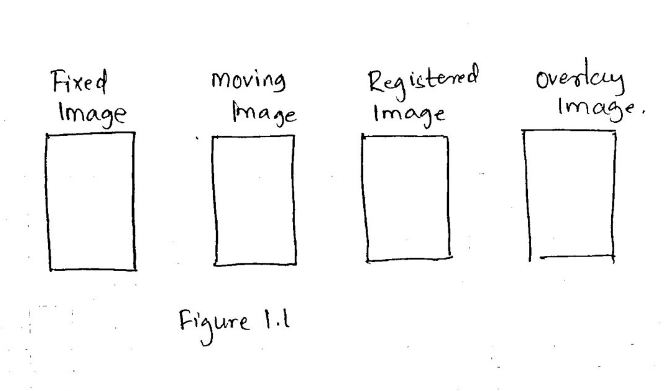
\includegraphics[width=0.7\columnwidth]{resources/chapter1/figure1.png}
		\caption{An image registration example}
		\label{fig:Registration}
	\end{figure}
	
	The above \ref{fig:Registration} shows an example of image registration of the drosophila larva brain obtained using the \textit{larvalign} software \cite{larvalign}. In this example, image registration was used to align two images of a drosophila larva, which were taken as 3D volumes but are shown here as maximum intensity projections for visualization purposes. The input images are referred to as the fixed image and the moving image, and the output is a registered image in which the moving image is aligned with the fixed image. This alignment can make it easier to analyze the images.
	
	\section{Motivation}
	Image registration can be done in two methods - deep learning method and traditional method. Both methods aim to align multiple images of the same or different objects, taken at different times or from different viewpoints. However, they differ in the approaches they take to achieve this goal.
	
	Traditional image registration methods typically rely on hand-crafted features or manually designed algorithms to align the images. On the other hand, image registration using deep learning methods relies on the use of neural networks to learn a mapping from the input images to the registered output. These methods can be more accurate and efficient than traditional methods, especially for complex images, as they are able to learn and adapt to the characteristics of the data. However, deep learning methods require a large amount of data for training.Traditional image registration can be prone to repeating errors and requires starting from scratch for each new image pair, whereas deep learning-based methods can learn from data and adapt to new image pairs more effectively.
	
	In this study, we aim to investigate the effectiveness of deep learning-based image registration in aligning brain scans of drosophila larvae and compare it to the traditional method. We will also explore the possibility of using auxiliary information, such as landmark points, to guide the learning process and improve the accuracy and efficiency of image registration.
	
	The focus of this thesis is to build upon the work presented in the \textit{larvalign} paper \cite{larvalign}, which is a 3D volume template and a registration method called \textit{larvalign} for aligning brain scans of drosophila larvae. While \textit{larvalign} showed promising results, it sometimes failed to accurately align images, particularly at the lower tip of the Ventral Nerve Cord (VNC) as shown in Figure \ref{fig:Registraion_Failure}.
	
	\begin{figure}[H]
		\centering
		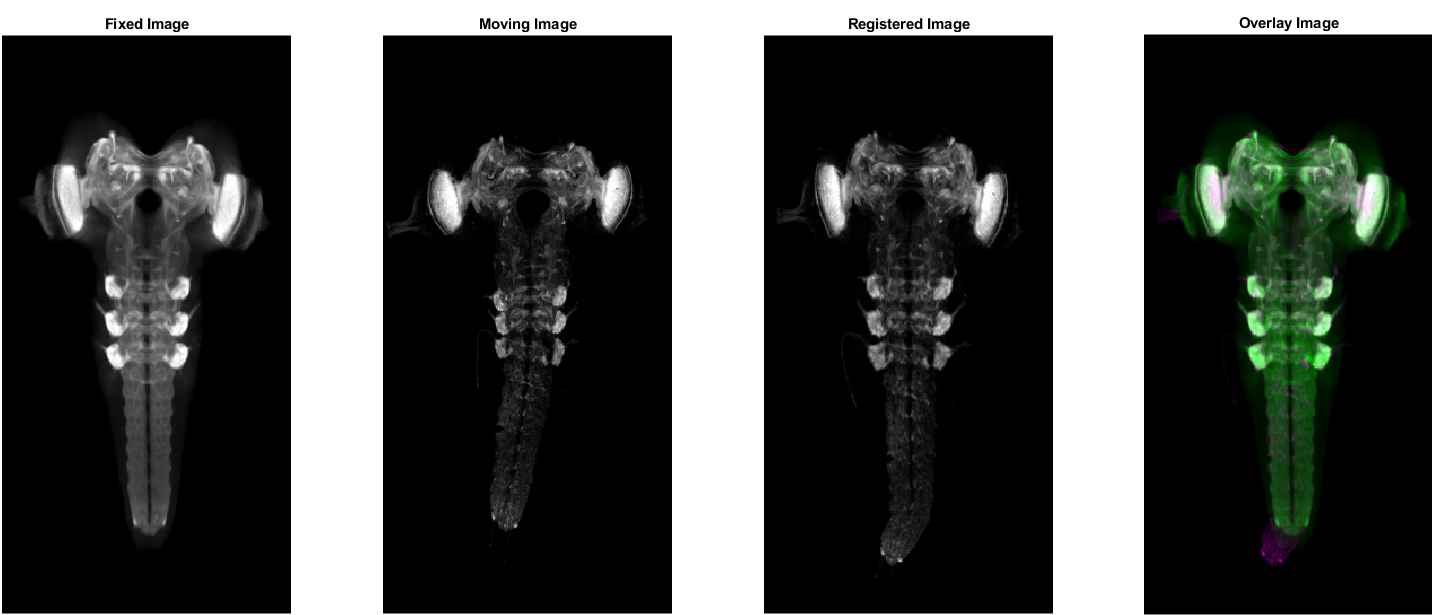
\includegraphics[width=\linewidth]{resources/motivation_fig_1.jpg}
		\caption{An example of a registration failure of \textit{larvalign} \cite{larvalign} at the lower tip of the Ventral Nerve Cord (VNC).}
		\label{fig:Registraion_Failure}
	\end{figure}
	
	The figure \ref{fig:Registraion_Failure} was plotted using MATLAB and displays four images as subplots in a row. 
	\begin{enumerate}
		\item The \textbf{Fixed or Template image} is the first image in the figure and is the image against which the registration is performed using the larvalign software.
		\item The \textbf{Moving or Subject image} is the second image in the figure and is the image that is being registered.
		\item The \textbf{Moved or Registered image} is the third image in the figure and is the result of the registration.
		\item The \textbf{Overlay image} is the fourth image in the figure and is an overlay between the fixed image and the moved image, which allows us to visually evaluate the quality of the registration.
	\end{enumerate}
	
	In the overlay image, green structures represent the fixed image and magenta structures represent the moved image. When the two images overlap perfectly, the intensity values are displayed.
	
	In this example case, the \textit{larvalign} software was unable to accurately align the moving image with the fixed image, as indicated by the protruding magenta structure at the lower tip of the Ventral Nerve Cord (VNC) in the overlay. This is an example of a case where \textit{larvalign} struggles to handle large deformations at the lower tip of the Ventral Nerve Cord (VNC) and consistently produces registration errors in these situations. This issue occurs repeatedly whenever we attempt to register these image pairs again.
	
	\textit{Larvalign} is a non-learning method for image registration, which means it cannot improve with experience. We are exploring the use of a learning-based method of registration that can adapt and potentially outperform larvalign. Deep learning techniques have been effective at learning to compute the deformation field between image pairs \cite{Balakrishnan_2019, de_Vos_2019, Wu, Fu_2020, 10.1007/978-3-319-66182-7_27}, and we expect this approach to be more efficient in terms of registration time compared to larvalign.
	
	\section{Objectives and Hypothesis}
	The goal of this thesis is to investigate whether deep learning techniques like Voxelmorph \cite{Balakrishnan_2019} can be used to improve the robustness and efficiency of image registration for biological scans of drosophila larva that may exhibit large deformations. We hypothesize that deep neural network architectures have the ability to learn complex, inherent features and can therefore be as efficient as \textit{larvalign} \cite{larvalign} in terms of accuracy in registration. Furthermore, we believe that by training these networks with more data, we can avoid the errors made by \textit{larvalign} \cite{larvalign} and that the prediction time for image registration using deep learning will be significantly faster, due to the ability of these networks to learn a function for computing the deformation field between pairs of images.
	
	
	\section{Organization}
	Finally, in this section we provide an overview of the structure of the thesis, highlighting the main chapters and subtopics that we will cover. This will help the reader to understand the organization of the study and how each chapter contributes to the research question.
	
	\begin{itemize}
		\item \textbf{Literature review}: This chapter presents an overview of the existing research on the topic of the study, highlighting the main findings and debates in the field.
		\item \textbf{Drosophila larva biology and an overview of machine learning techniques}: This chapter provides an overview of Drosophila larva biology and a summary of the machine learning techniques that will be used in the study.
		\item \textbf{Methods and Implementations}: This chapter describes the research design, sample, and data collection and analysis procedures used in the study. It provides enough detail for readers to understand and replicate the study.
		\item \textbf{Results}: This chapter presents the findings of the study, including tables, figures, and other visualizations. In addition, we will conduct several ablation studies to explore the effect of different parameters on training.
		\item \textbf{Discussion}: This chapter interprets and contextualizes the results of the study, discussing their implications and limitations in relation to the literature review and research question. It also identifies areas for future research.
		\item \textbf{Conclusion}: This chapter summarizes the main findings and implications of the study, and will highlight the contribution of the research to the field.
	\end{itemize}
	
	\chapter{Literature review}
	\label{chap:litreture}
	Over the past few decades, given the numerous applications of image registration, a plethora of methods have been proposed. Until the success of AlexNet \cite{AlexNet} in the 2012 ImageNet competition, many of the proposed methods formulated the registration problem as a physical problem to minimize the energy function \cite{THIRION1998243} \cite{536892} \cite{5193151} \cite{5338015} \cite{Avants2011ARE} \cite{1009381}. The success of AlexNet led to increased confidence in deep learning techniques and their widespread use in research. This can be seen in Figure \ref{fig:no_of_papers}, which shows the increase in Deep Learning-based image registration work after 2012.
	
	The adaptation to deep learning techniques led to exceptional performance results in many computer vision tasks such as object recognition, image segmentation, image classification, etc., which could not be achieved before, and the popularity of deep learning methods increased rapidly.
	
	Not surprisingly, the current state-of-the-art methods for image registration are also based on deep learning methods, which are also used in this work. Traditional optimization methods minimize the dissimilarity function (or maximize the similarity function) between the fixed image and the moving image with respect to the registration parameters in an iterative process. In modern deep learning methods, the model is trained to learn the mapping between the fixed image and the moving image by optimizing an objective or cost function to perform registration in a single shot rather than iteratively. Although the training process can be resource intensive, the time required to perform registration after training a model is much less than the time required to perform mathematical optimization from scratch for each new image pair. Therefore, the methods can generally be divided into two types: traditional non-learning methods and modern deep learning methods. We'll talk about these in the next two sections, \nameref{section:traditional} and \nameref{section:dl}.
	
	\section{Traditional methods}
	\label{section:traditional}
	
	Thirion's Demons algorithm \cite{THIRION1998243} has been a popular choice for deformable registrations since the beginning of this century due to its linear complexity and simple implementation. The main idea of this work was to consider the object boundaries in one image as a semipermeable membrane and allow the other image, considered as a deformable grid model, to diffuse through these semipermeable boundaries by the action of effectors called demons located at these boundaries. The concept of demons was introduced by Maxwell in the 19th century to illustrate a paradox in thermodynamics, and this concept has been successfully adapted to image processing. If we want to match a moving image \emph{M} with a fixed image \emph{F}, it is assumed that the contour of an object \emph{O} in \emph{F} is a membrane and several demons are scattered on the contours of this object \emph{O}. These demons act as local effectors, pushing the moving deformable model \emph{M} to the inside of \emph{O} if the corresponding point of \emph{M} is labeled "inside" or to the outside of \emph{O} if it is labeled "outside".
	Image matching is an iterative process to find the transformation form \emph{T} that is the  evolution of a family of transformations \{$T_0$, $T_1$, ..... $T_i$, ..\} $\subset$ $\tau$ (where $\tau$ is the set of admissible deformations).
	
	Starting from an identity deformation {$T_0$}, for each iteration, the elementary force for each demon at the object boundary of the fixed image is calculated. From all elementary forces of the demons, the deformation $T_{i+1}$ of $T_i$ is calculated. The following figure \ref{fig:demons} represents this iterative scheme.
	
	\begin{figure}[H]
		\centering
		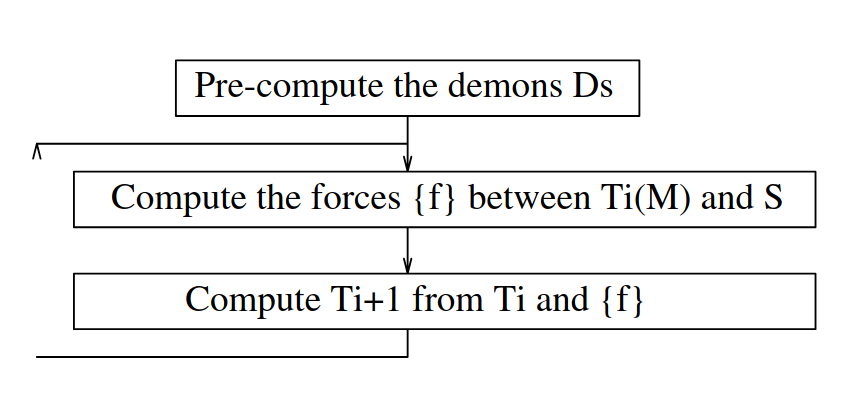
\includegraphics[width=0.7\columnwidth]{resources/chapter2/demons.png}
		\caption{Iterative scheme in the case of diffusing models. \cite{THIRION1998243}}
		\label{fig:demons}
	\end{figure}
	
	One of the pioneering ideas in the field of large deformation registration was Christensen's modeling of the image as a fluid \cite{536892}. The image registration problem was formulated as a semilinear partial differential equation (PDE) system on the velocity field of the deformation, and it was shown how fixed point iteration generates a sequence of linear PDE systems. In \cite{5193151}, the demon algorithm was modified to perform curvature and fluid registration.
	
	As mentioned earlier, there are a plethora of methods that have been proposed for image registration. Unfortunately, however, no universal method can be developed that is suitable for all registration problems. This may be due to the variety of images, assumed deformation types, required registration accuracy, application-dependent features, and other factors. To alleviate this problem, Klein et al. \cite{5338015} in 2010 developed a software toolbox called \emph{elastix} for intensity-based registration problems specifically used in medical image processing. The \emph{elastix} software contains various optimization methods, multiresolution methods, interpolators, samplers, transformation models, and cost functions which is very helpful for the user to quickly compare different registration methods and select a satisfactory configuration for a particular application. \emph{{larvalign}} \cite{larvalign} proposes such a method using \emph{elastix}. \emph{{larvalign}} \cite{larvalign} is an automatic and semi-automatic registration procedure, which is also the impetus for this thesis. In the following subsection, we shall talk more about what \emph{{larvalign}} is and the results it achieved.
	
	\subsection{\emph{larvalign}}
	As mentioned earlier, \emph{{larvalign}} \cite{larvalign} is the stimulus for this work, i.e., this work is an extension of the work of \emph{{larvalign}} \cite{larvalign}. \emph{{larvalign}} \cite{larvalign} is both a standard template of the larval brain of the fruit fly \emph{Drosophila melanogaster} and an automatic and semi-automatic registration method for registering different scans of the larval brain to this standard template. The \emph{{larvalign}} \cite{larvalign} software package performs a specific sequence of image processing steps optimized specifically for the registration of microscopic images of the central nervous system (CNS) of third instar Drosophila larvae. The following is a brief overview of the registration algorithm, the evaluation of the results, and finally the results itself in \emph{{larvalign}} \cite{larvalign}.
	
	\subsubsection{Registration Algorithms}
	\label{subsubsection:registration_algo}
	Image registration in \emph{{larvalign}} is performed in two steps: global alignment of images (linear/affine/rigid registration) and local alignment of images (nonlinear/deformable/non-rigid registration).
	
	The global alignment serves as initialization for the nonlinear registration. During the acquisition of brain samples, the samples can be randomly aligned and also mirrored in the z-direction. The goal of global alignment is to ensure that these acquired brain scans (moving images) have approximately the same orientation, size, and are in the same slice order in the z-direction as the standard template larval brain.  Therefore, linear (affine) registration prior to nonlinear (deformable) registration would greatly facilitate the implementation of the non-rigid transformation.
	
	Local alignment was performed using both non-parametric methods (variational methods) and parametric methods (B-spline models). Both methods were empirically evaluated to select the best of the two. Both categories have their own state-of-the-art toolkit for biomedical image registration, \emph{ANTs} \cite{Avants2011ARE} and \emph{elastix} \cite{5338015}, where \emph{ANTs} image registration is best known for its symmetric diffeomorphic registration (SyN) algorithm \cite{Avants2008SymmetricDI}. An initial experiment was performed to \emph{ANTs} SyN and \emph{elastix} B-spline registration approach for pairwise nonlinear registration. Although comparable results were obtained with both methods, it was found that registration with \emph{ANTs} took more than 8 hours, whereas registration with \emph{elastix} took about 4 minutes. Since the goal was accurate and \emph{fast} image registration, the \emph{elastix} approach was chosen.
	
	\subsubsection{Assessment}
	\label{subsubsection:assessment}
	In addition to the visual inspection of the registered image, a quantitative value was defined to measure the quality of the registra¸tion. Although the correlation between the registered image and the fixed image captures the misalignment, such global measurements usually do not account for the local errors. To quantify local registration errors, statistical descriptors were developed for the regions at the entry points of the Ventral Nerve Cord (VNC) and thoracic nerve, similar to those used by Muenzing et al \cite{Muenzing},. These descriptors were defined as VNC Terminal Error Indicator (\textbf{VI}) and Thoracic Nerve Error Indicator (\textbf{TI}), respectively. If these indicators had a value of less than 50\%, this was an indication of a possible registration error. Apart from these two, another error called landmark registration error (\textbf{LRE}) was defined, which was nothing but the average of the Euclidean distance between all landmarks in the fixed image and the registered image.
	
	Up to this point, registration is completely automatic and does not require human intervention. However, for those cases where \textbf{VI} and \textbf{TI} scored less than 50\%, a framework for registration based on landmarks was developed as a fallback strategy. In the event that VNC registration fails (\textbf{VI} score less than 50 \%), two landmarks were provided to guide this semi-automatic registration. In the event that thoracic registration failed (\textbf{TI} score less than 50 \%), six landmarks were placed at all six entry points of the thoracic nerve.	In contrast to automatic deformable registration, where only the correlation (NCC or MMI) between images controls the registration process, in semi-automatic deformable registration two similarity metrics control the registration process - the correlation metric and the Euclidean distance between the corresponding points \cite{inproceedings}.
	
	In the tabular data provided in \textit{larvalign} \cite{larvalign} it can be seen that for the partially failed registrations, landmark registration error (\textbf{LRE}) decreased after the semi-automatic registration was performed.
	
	\subsubsection{Results}
	\label{subsubsection:result}
	The proposed \emph{{larvalign}} registration method achieved an average landmark registration error (\textbf{LRE}) of \textbf{2.5 micrometers ± 1.5 micrometers} for the highest image quality data set, which is within the range of empirically measured human intra-rater variation measured on the same data set. However, the average landmark registration error (\textbf{LRE}) was \textbf{6.9 micrometers ± 6.4 micrometers} for the worst image quality within the representative data set, but it was noted that the intra-rater variation was measured on the high quality data and the baseline error could also be higher for the worst image quality data set.
	
	\section{Deep Learning Methods}
	\label{section:dl}
	
	Deep Learning (DL) belongs to a class of machine learning that uses neural networks with a large number of layers to learn the representation of the data and solve the task at hand. DL architectures had been limited in their ability to solve the then problems due to the vanishing gradient and the problem of overfitting. However, due to the availability of large datasets, large computational power in the form of GPUs and TPUs, and novel algorithms for training such deep networks, there has been a resurgence of interest in this concept. Recent works have also shown that they can even perform better than humans in some visual recognition tasks.
	
	When it comes to image registration, there are broadly three strategies that are prevalent in the current deep learning literatures: (1) using deep learning networks to estimate discriminate features for two images to drive an iterative optimization strategy, (2) using deep learning regression networks to directly predict transformation parameters, and (3) using deep learning networks to directly predict the deformation field. \cite{Litjens_2017}
	
	Wu et al. \cite{7314894} \cite{Wu} were the first ones to use deep learning to obtain application specific feature in contrast to the supervised feature extraction or handcrafted feature selection methods, and then the learnt features were deployed to the classical Demons \cite{VERCAUTEREN2009S61}, \cite{10.1007/10704282_64}, \cite{10.1007/978-3-540-85990-1_117}, \cite{10.1007/978-3-642-24446-9_3}, \cite{Peyrat} and HAMMER methods \cite{Wu2010TPSHAMMERIH}, \cite{Shen} with defined interpolation strategy, transformation model, and optimization alogirthm. These features were learnt from the data and hence is optimal representation for specific dataset. Thus, the then state-of-the-art registration methods were imporved by integrating these feature representations via deep learning. However, the registration process is still slow because the later transformation estimation is still iterative. Thus, methods to directly predict the transformation parameters have been proposed such that the registered image can be obtained directly by warping the moving image with the predicted transformation parameters.
	
	\begin{figure}[H]
	\centering
	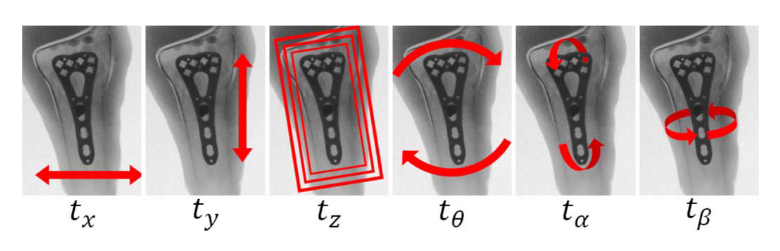
\includegraphics[width=0.7\textwidth]{resources/chapter2/tx_parameters.png}
	\caption{6 transformation parameters in a 3D transformation. \cite{7393571}}
	\label{fig:tx_parameters}
	\end{figure}
	
%	\begin{wrapfigure}{r}{0.5\textwidth}
%		\begin{center}
%			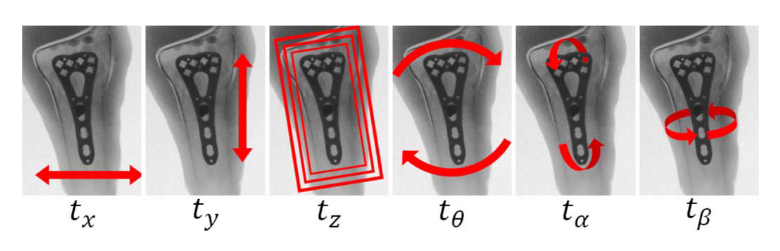
\includegraphics[width=0.5\textwidth]{resources/chapter2/tx_parameters.png}
%		\end{center}
%		\caption{6 transformation parameters in a 3D transformation. \cite{7393571}}
%		\label{fig:tx_parameters}
%	\end{wrapfigure}	
	
	Miao et al. \cite{7393571} were the first to use deep learning network to predict rigid transformation parameters. A rigid-body 3D transformation \emph{T} can be parameterized by a vector \emph{\textbf{t}} with 6 components of which 3 are in-plane (the translation parameters \emph{\textbf{$t_x$}} and \emph{\textbf{$t_y$}}, and rotation parameter \emph{\textbf{$t_\theta$}}) and 3 are out-of-plane (the translation parameter \emph{\textbf{$t_z$}} and rotation parameters \emph{\textbf{$t_\alpha$}} and \emph{\textbf{$t_\beta$}}) transformation parameters as shown in \ref{fig:tx_parameters}. A convolutional neural network (CNN) was used to predict the transformation parameters. Instead of regressing all parameters together, they were divided into three groups and regressed hierarchically.
	
	
	
	%\begin{wrapfigure}{r}{0.5\textwidth}
	%	\begin{center}
	%		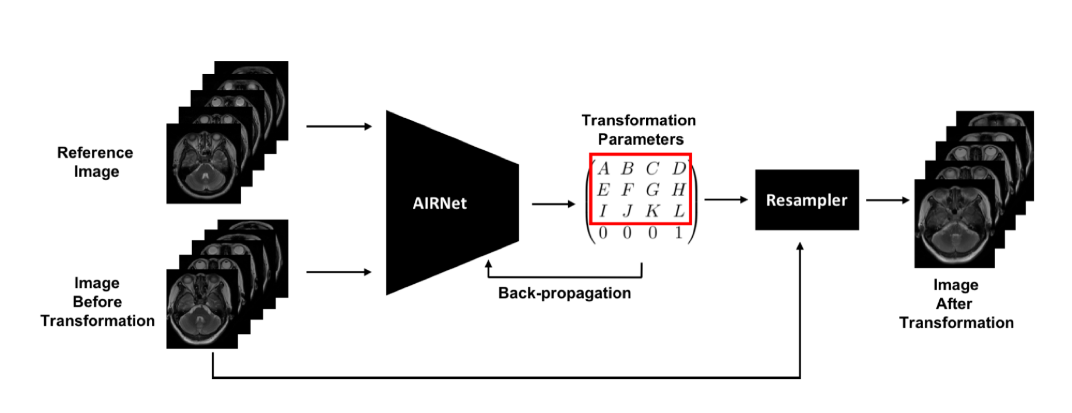
\includegraphics[width=0.5\textwidth]{resources/chapter2/AIRNet.png}
	%	\end{center}
	%	\caption{Workflow of \cite{https://doi.org/10.48550/arxiv.1810.02583} image registration framework.}
	%	\label{fig:AIRNet}
	%\end{wrapfigure}
	
	Chee et al. \cite{https://doi.org/10.48550/arxiv.1810.02583} employed a CNN to predict all transformation parameters simultaneously, rather than predicting them in groups and then applying them in a hierarchical fashion. In this framework, their Affine Image Registration Network (AIRNet) took two images and outputs the rigid transformation parameters. The moving image is then warped by the resampler using transformation matrix. The training loss function was mean-squared error of the estimated transformation parameters.
	
	%\begin{figure}[H]
	%	\centering
	%	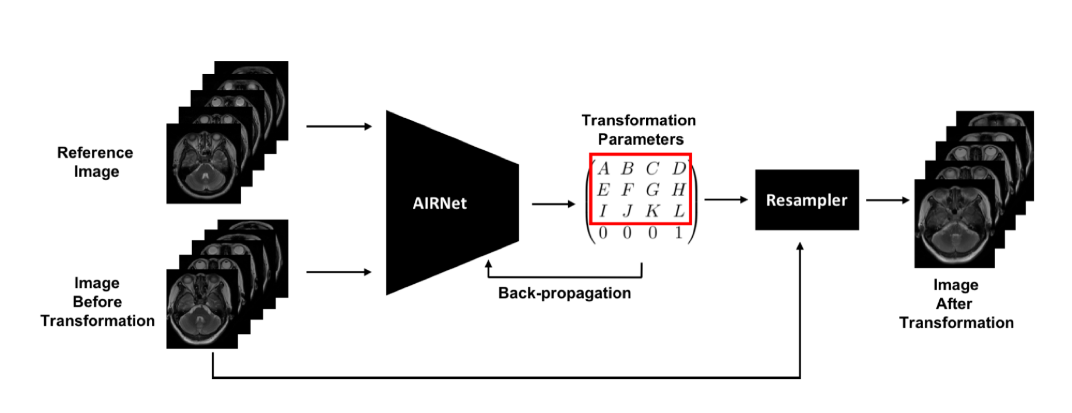
\includegraphics[width=0.7\columnwidth]{resources/chapter2/AIRNet.png}
	%	\caption{Workflow of \cite{https://doi.org/10.48550/arxiv.1810.02583} image registration framework.}
	%	\label{fig:AIRNet}
	%\end{figure}
	
	Yang et al. \cite{10.1007/978-3-319-46976-8_6}, Rohe et al. \cite{Roh2017SVFNetLD}, Jun et al. \cite{Jun}, Sokooti et al. \cite{10.1007/978-3-319-66182-7_27} and many others used deep learning approaches to predict the deformation field in a supervised fashion either with ground truth data or synthetic data.
	
	Interestingly, in one another work by Yang et al. \cite{https://doi.org/10.48550/arxiv.1804.11024}, Generative Adversarial Network was used to estimate the rigid transformation. Generator network was trained to predict the rigid transformation parameters, while the discriminator was trained to discern between the images that were warped with predicted transformation parameters and the images that were warped with the ground truth transformation parameters. Both Eucledian distance to ground truth and an adversarial loss term were used to construct the loss function.
	
	\subsection{Unsupervised Transformation Estimation}
	Despite the success of the above methods, the difficulty of obtaining reliable ground truth in the form of a warped image or deformation field is a major obstacle. This has motivated a number of research groups to explore unsupervised approaches. In this thesis also, an unsupervised approach is pursued, and thus this separate subsection is devoted to it in order to express its importance.
	
	A key innovation that has been useful for all work following the unsupervised method is the spatial transformer network (STN) \cite{NIPS2015_33ceb07b}. The spatial transformer network is a differentiable module that can be inserted into existing convolutional architectures, giving neural networks the ability to spatially transform feature maps. Since it is a differentiable module, it can also be trained together in an end-to-end fashion through backpropagation. In the paper, "A Survey on Deep Learning in Medical Image Registration", \cite{Haskins_2020} a nice visualization aptly describes the workflow of unsupervised deep learning methods for registration.
	
	\begin{figure}[H]
		\centering
		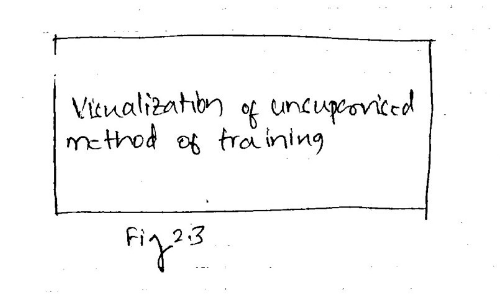
\includegraphics[width=0.7\columnwidth]{resources/chapter2/figure2.png}
		\caption{Visualization of unsupervised method of training deep neural networks for registration. \cite{Haskins_2020}}
		\label{fig:unsupervised_visualization}
	\end{figure}
	
	One of the important works in this area is by de Vos et al. \cite{de_Vos_2019}. In their work they proposed a Deep Learning Image Registration (DLIR) framework for unsupervised affine and deformable registrations. The framework is trained for image registration by exploiting image similarity between fixed and moving image pairs. In the DLIR framework, the transformation parameters are learnt by analysing the fixed and the moving image pairs. The predicted transformation parameters are then used to make a dense displacement vector field (DVF). DVF is used to resample the moving image into a warped image. Unlike many works that expects the moving image to be already to affinely aligned with the fixed image, the DLIR is designed for affine as well as deformable registration. Additionally, the framework also supports multi-stage ConvNets for registration of coarse-to-fine complexity in multiple-levels and multiple image resolutions by stacking ConvNets in a serial fashion. It is also said that such hierarchical mutli-stage strategy makes conventional iterative image registration less sensitive to local optima and image folding \cite{10.1007/3-540-45468-3_69}. Each stage is trained for its specific registration task, while keeping each of its weights fixed. After training, the multi-stage ConvNet is applied for one-shot image registration, similar to a single ConvNet.
	
	\begin{figure}
		\centering
		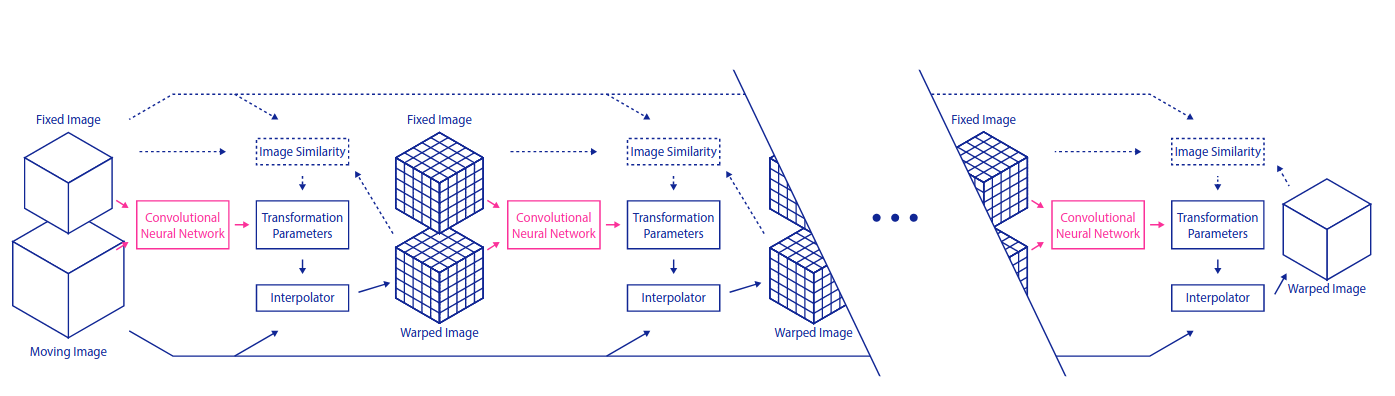
\includegraphics[width=\columnwidth]{resources/chapter2/DLIR.png}
		\caption{Schematic representation of the DLIR framework for hierarchical training of multi-stage ConvNet for multi-resolution and multi-level image registration. \cite{de_Vos_2019}}
		\label{fig:DLIR}
	\end{figure}
	
	In the next section, the current state-of-the-art methods which are also unsupervised is explained in detail.
	
	\section{State-of-the-art methods}
	There are many proposed methods in the literature for learning a function for medical image registration using convolutional neural networks in an unsupervised manner. In this work, we consider some of these methods, which are the current state of the art, as base methods and adapt them to achieve a successful registration result for our larval brain scans.
	
	\subsection{VoxelMorph: An Unsupervised Learning Model for Deformable Medical Image Registration} 
	Like many other deep learning methods, the method proposed in VoxelMorph \cite{8579062} \cite{Balakrishnan_2019} also formulate registration as a function that maps an input image pair to a deformation field that matches the moving and fixed images. However, unlike other methods, two different training strategies were proposed in this work. In the first (unsupervised) setting, the model is trained to maximize the similarity between the fixed image and the registered image based on the image intensities. In the second setting, auxiliary information in the form of anatomical segmentations were used to steer the network in the right direction of learning. It was found that the model trained with auxiliary information performed better than the model trained without at the test time. The performance of both settings was comparable to the then state-of-the-art methods.
	
	3D MR scans of the human brain from healthy and sick people of different age groups were used for the study. In this work, more attention was paid to the slower deformable transformation than to the comparatively faster affine transformation. Therefore, it is assumed that the moving image and the fixed image are already affine aligned.
	
	The registration problem was formulated to find the optimal displacement vector field such that the dissimilarity between the fixed and registered images is the smallest. In addition, a smoothing loss was included to act as a regularizer to enforce a spatially smooth deformation.
	
	
	% https://oeis.org/wiki/List_of_LaTeX_mathematical_symbols
	% https://www.overleaf.com/learn/latex/Aligning_equations_with_amsmath
	\begin{equation} \label{loss_vxm}
	\begin{split}
	\hat{\phi} & = \argmin_\phi \mathcal{L}(f,m,\phi) \\
	& = \argmin_\phi (\mathcal{L}_{sim}(f,m \circ \phi) + \lambda \mathcal{L}_{smooth}(\phi))
	\end{split}
	\end{equation}
	
	where $m$ is moving image, $f$ is fixed image, $\phi$ is the deformation field, and $m \circ \phi$ represents $m$ warped by $\phi$, function $\mathcal{L}_{sim}(\cdot,\cdot)$ measures the similarity between the two input images, $\mathcal{L}_{smooth}(\cdot)$ imposes regularization, and $\lambda$ is the regularization trade-off parameter.
	
	The common metrics used for $\mathcal{L}_{sim}$ include intensity mean squared error, normalized cross correlation, and mutual information. The latter two are useful when volumes have varying intensity distributions and contrasts.
	
	\subsubsection{VoxelMorph CNN Architecture}
	
	Figure \ref{fig:vxm} depicts the network used in VoxelMorph. The network accepts both moving image $m$ and fixed image $f$ which is further concatenated into a 2 channel 3D image before fed to encoder-decoder architecture with skip connections. 3D convolutions in both the encoder and decoder stages use a kernel size of 3, a stride of 1, and same padding. Each convolution is followed by a leakyReLU layer with parameter 0.2. The convolution layers capture hierarchical features of the input image pair, to estimate $\phi$.
	
	In the encoder, max-pooling is performed to reduce the spatial dimensons in half at each layer. Thus, successive layers of the encoder operate over coarser representations of the input. This multilayer encoder network is used to transfer the high-dimensional 3D image patches into the low-dimensional feature representations.
	
	In decoder, alternate between upsampling, convolutions and skip connections are done. The decoder network is used to recover 3D image patches from the learned low-dimensional feature representations, acting as feedback to refine the inferences in the encoder network.
	
	\begin{figure}[H]
		\centering
		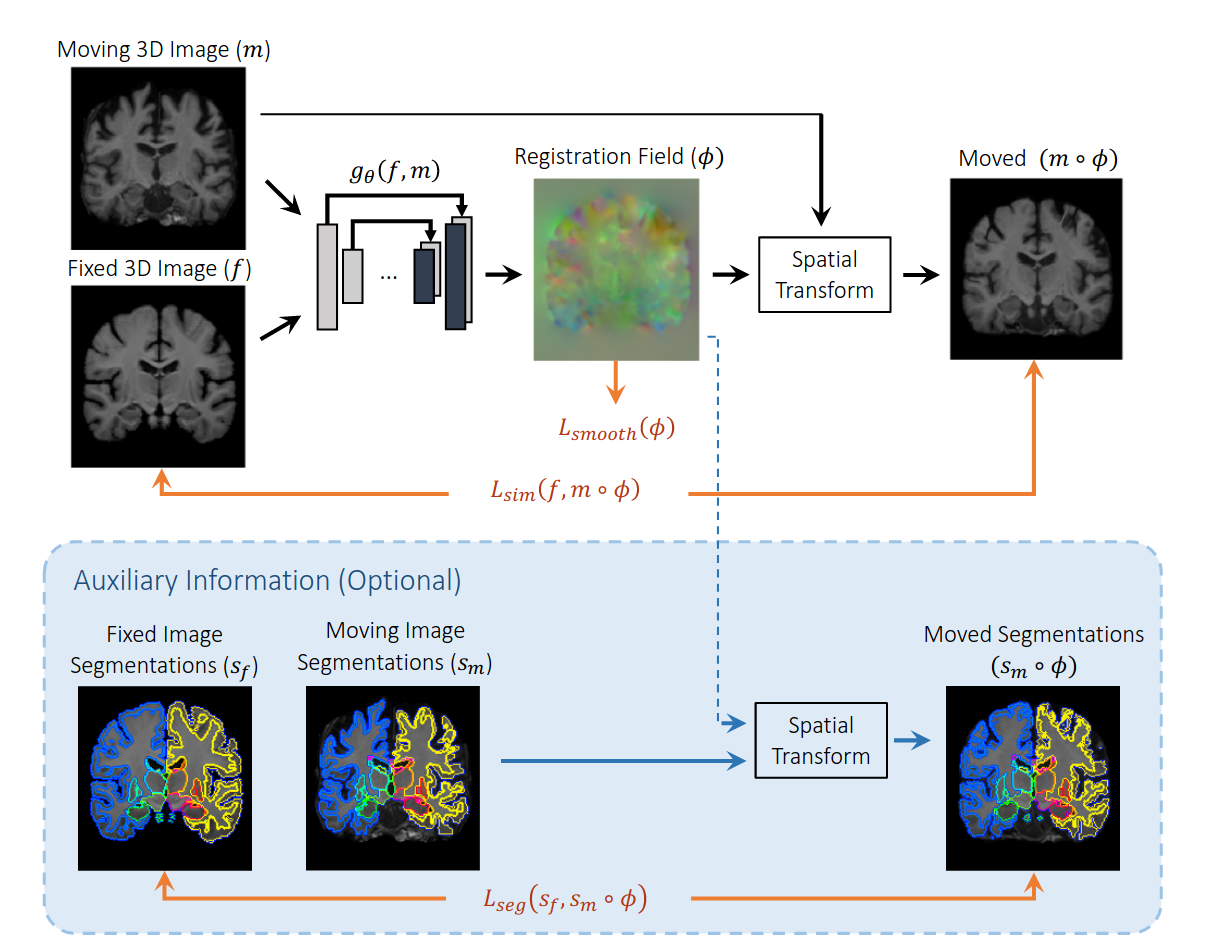
\includegraphics[width=0.9\columnwidth]{resources/chapter2/vxm.png}
		\caption{Overview of the VoxelMorph method. \cite{Balakrishnan_2019}}
		\label{fig:vxm}
	\end{figure}
	
	An important architectural constraint is that the receptive fields of the convolutional kernels of the smallest layer should be at least as large as the maximum expected displacement between corresponding voxels in $f$ and $m$.
	
	\begin{figure}[H]
		\centering
		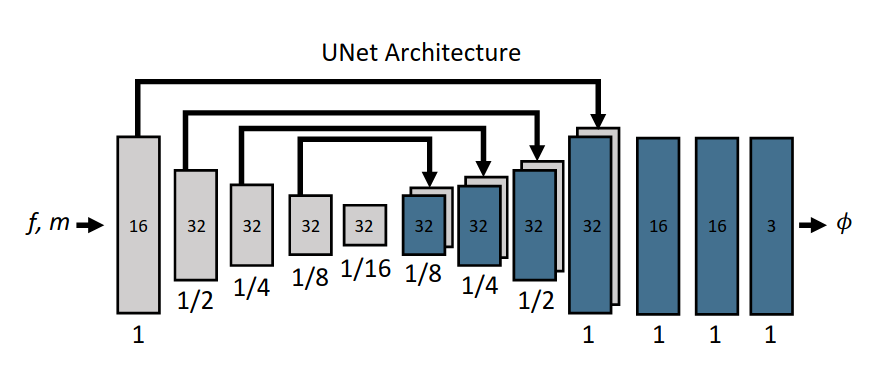
\includegraphics[width=0.8\columnwidth]{resources/chapter2/vxm_unet.png}
		\caption{Implementation of the U-Net convolution architecture. Each rectangle represents a 3D volume created from the previous volume using a 3D convolutional network layer. The spatial resolution of each volume with respect to the input volume is given below. Multiple 32-filter convolutions are used in the decoder, each followed by an upsampling layer to bring the volume back to full resolution. The arrows represent skip connections that chain encoder and decoder functions. \cite{Balakrishnan_2019}}
		\label{fig:vxm_unet}
	\end{figure}
	
	The figure \ref{fig:vxm_result} shows the average dice scores and runtime results for affine alignment, ANTs, NiftyReg and VoxelMorph. Standard deviations across structures and subjects are in parantheses. The average Dice score is computed over all the structures and subjects.
	
	\begin{figure}[H]
		\centering
		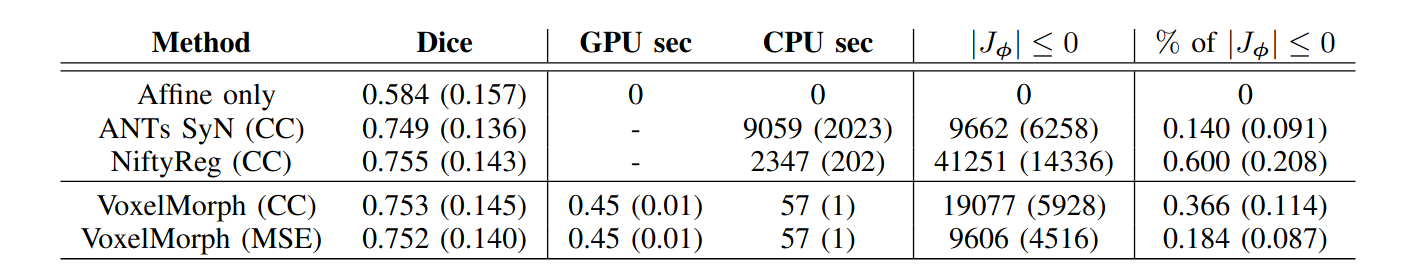
\includegraphics[width=\columnwidth]{resources/chapter2/vxm_result.png}
		\caption{Average Dice scores and runtime results for affine alignment, ANTs, NiftyReg and VoxelMorph. \cite{Balakrishnan_2019}}
		\label{fig:vxm_result}
	\end{figure}
	
	In another setup, the trained VoxelMorph was tested on the (unseen) Buckner40 dataset containing 39 scans. VoxelMorph with instance specific optimization was also performed. The dice scores in \ref{fig:vxm_result_2} show that VoxelMorph using cross correlation loss behaves comparably to ANTs and NiftyReg using the same cost function. Further, VoxelMorph with instance-specific optimization improved the results.
	
	\begin{figure}[H]
		\centering
		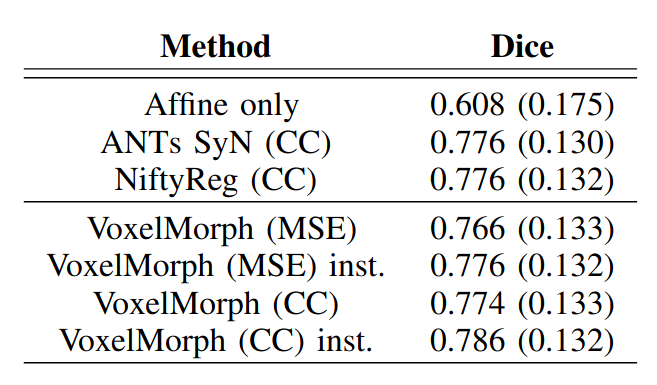
\includegraphics[width=0.5\columnwidth]{resources/chapter2/vxm_result_2.png}
		\caption{Results for manual annotation experiment. \cite{Balakrishnan_2019}}
		\label{fig:vxm_result_2}
	\end{figure}
	
	Finally, the authors conclude that the VoxelMorph is a general learning model, and is not limited to any particular image type or anatomy - may be useful in medical image registration applications such as cardiac MR scans or lung CT images. Also, authors are of the opinion that with approporiate loss functions like mutual information, the model can also perform multimodal registration.
	
	\subsection{Cascade Networks for Unsupervised Medical Image Registration}
	Following the success of Voxelmorph \cite{Balakrishnan_2019}, improvised frameworks like Volume Tweening Network (VTN) \cite{8889674} and architectures like Recursive Cascaded Networks \cite{Zhao_2019} were proposed. Both the methods aimed at addressing the issues where the registration meant resolving large displacement fields.
	
	Although the authors note in the VoxelMorph paper \cite{Balakrishnan_2019} that the model may be useful for medical image registration applications such as MR scans of the heart or CT scans of the lung, Zhao et al. \cite{8889674} note that VoxelMorph does not work well when large shifts are present between images. Therefore, both papers \cite{8889674} and \cite{Balakrishnan_2019} offer a solution for dealing with such scenarios where large deformation fields are present by cascading the networks. In both the methods, final deformation field is a composition of field from the subnetworks. That is, the final flow prediction is composed of an initial affine transformation and $\phi_1$, $\phi_2$, $\cdots$, $\phi_n$, each of which only performs a rather simple displacement.
	
	\begin{figure}[H]
		\centering
		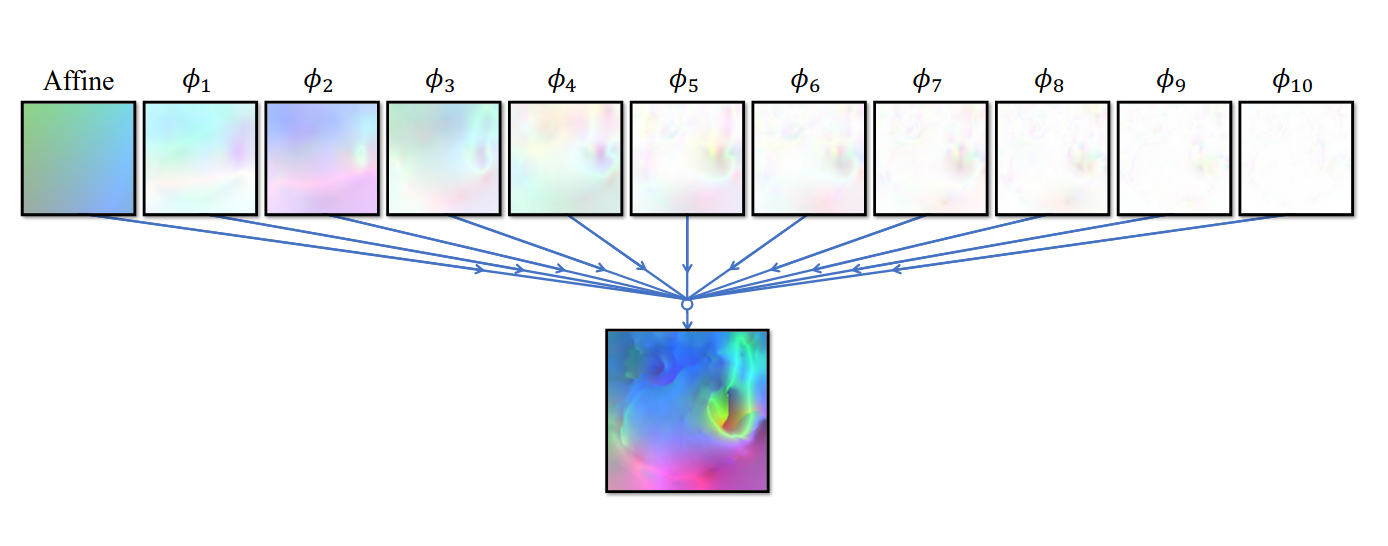
\includegraphics[width=\columnwidth]{resources/chapter2/recursive_cascade_flowfield.png}
		\caption{Composition of deformation fields. Flow fields are drawn by mapping the abosolute value of the three components (x, y, z) of flow displacements into color channels (R, G, B) respectively. White area indicates zero displacement. \cite{Zhao_2019}}
		\label{fig:recursive_cascade_flowfield}
	\end{figure}
	
	Both VTN \cite{8889674} and DLIR \cite{de_Vos_2019} stack their networks. However, both are limited to a small number of cascades. DLIR trains each cascade one by one, i.e., after fixing the weights of previous cascades. VTN, in contrast, jointly trains the cascades measuring the similiarity between all successively warped images and the fixed image. The figure below \ref{fig:vtn} shows the Volume Tweening Network (VTN) \cite{8889674}. Each registration subnet is responsible for determining the deformation field between the fixed image and the current moving image. The moving image is repeatedly distorted according to the deformation and fed into the next layer of cascaded subnetworks.
	
	\begin{figure}[H]
		\centering
		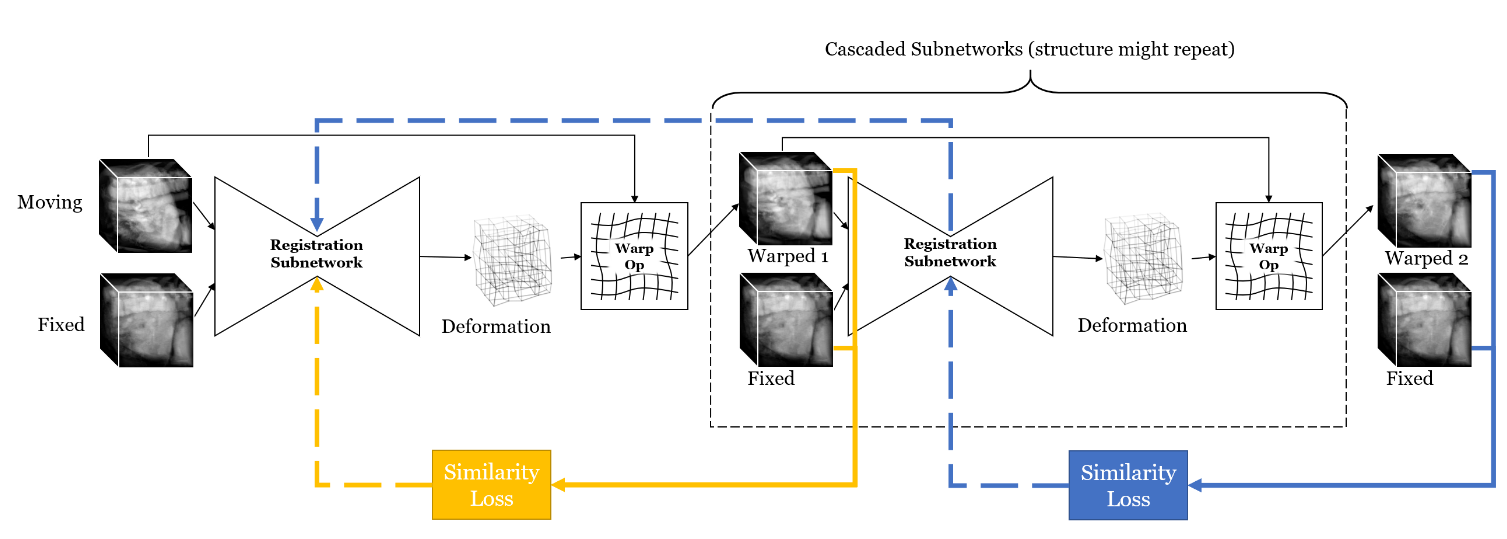
\includegraphics[width=\columnwidth]{resources/chapter2/vtn.png}
		\caption{Illustration of the overall structure of the Volume Tweening Network (VTN) and the back-progression of gradients. Solid lines indicate how the loss is computed and the dashed lines indicate how gradients back-propagate\cite{8889674}}
		\label{fig:vtn}
	\end{figure}
	
	Zhao et al. \cite{Zhao_2019} note that such a training method does not allow progressive registration of images. They refer to these as non-cooperative cascades because they learn their own targets independently of each other's existence, making further improvement unlikely even if more cascades are performed. Therefore, Zhao et al. \cite{Zhao_2019} propose the recursive cascade architecture, which allows unsupervised training of an unlimited number of cascades cascaded in a cooperative manner on any existing base network.
	
	The architecture of the proposed recursive cascaded network is shown in the figure below \ref{fig:recursive}. The difference between this architecture and the VTN is that the similarity is now measured only on the final warped image, so that all cascades can learn progressive alignments together.
	
	\begin{figure}[H]
		\centering
		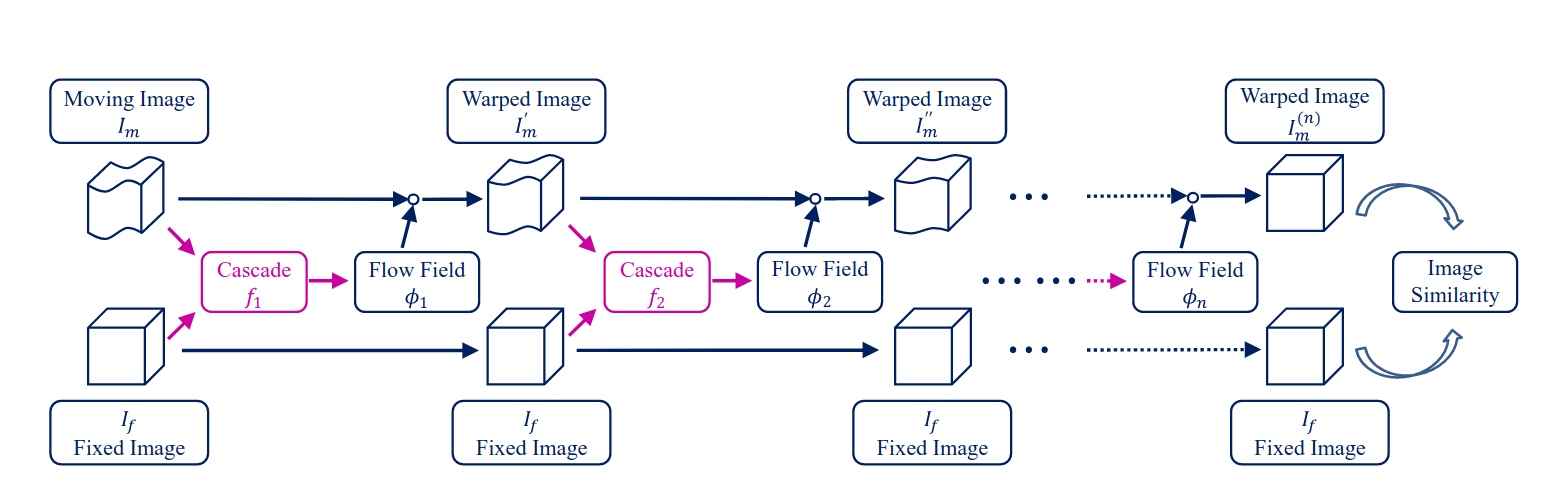
\includegraphics[width=\columnwidth]{resources/chapter2/recursive.png}
		\caption{Illustration of the recursive cascade architecture. Circle denotes a composition. The unsupervised end-to-end learning is guided by the image similiarity between $I_m^{(n)}$ and $I_f$.\cite{Zhao_2019}}
		\label{fig:recursive}
	\end{figure}
	
	The following figure \ref{fig:recursive_result} shows the performance of the recursive cascade network architectures for the SILVER, LiTS, and LSPG datasets. For testing purposes, both VoxelMorph and VTN were chosen as the base network here, and an empirical evaluation was performed. In all cases, the cascaded architecture performed better than the simple network alone.
	
	\begin{figure}[H]
		\centering
		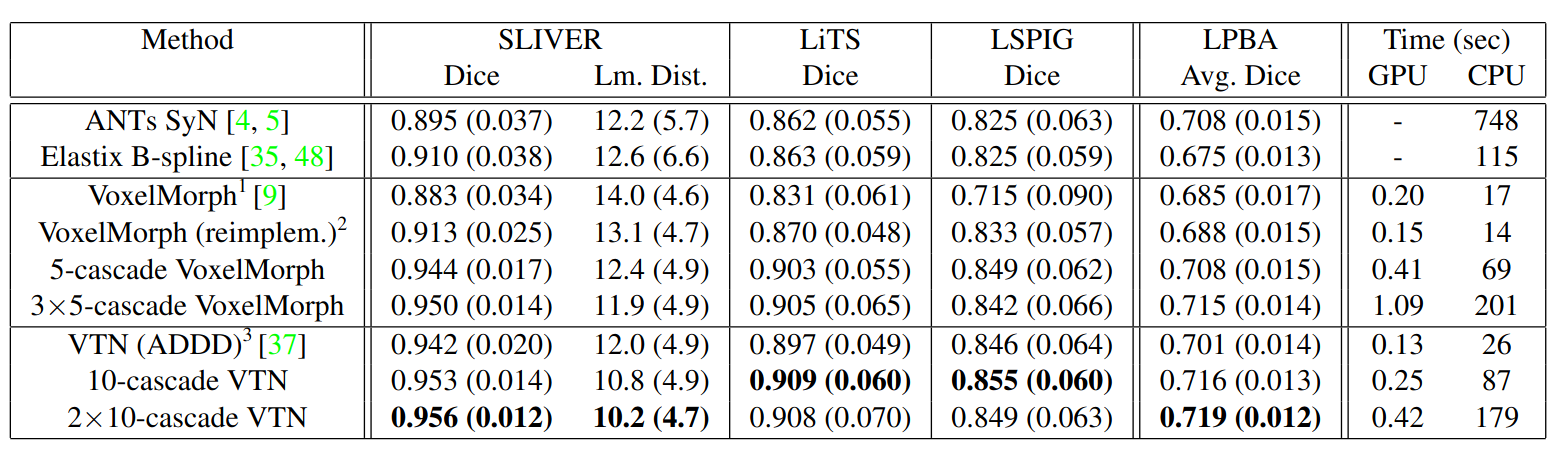
\includegraphics[width=\columnwidth]{resources/chapter2/recursive_result.png}
		\caption{Comparison among traditional methods (ANTs SyN and Elastix B-spline), baseline networks (VoxelMorph and VTN), and proposed recursive cascaded networks with and without shared-weight cascading. $r$ x $n$ -cascade means that every deformable cascade is repetitively applied for r times during testing, using the proposed shared-weight cascading method. \cite{Zhao_2019}}
		\label{fig:recursive_result}
	\end{figure}
	
	
	After studying the literature, we decided to use VoxelMorph as the base model and incorporate concepts of VTN, DLIR, and recursive cascading networks for better performance. The cascading of the networks will be implemented in a coarse-to-fine fashion, similar to the image pyramid used in traditional image registration methods and proven for many years.
	
	
	\chapter{Drosophila larva biology and an overview of machine learning techniques}
	The Drosophila larva is a widely studied model organism in the field of biology, due to its short lifespan and ease of genetic manipulation. In this chapter, we will provide an overview of the biological stages of Drosophila larva development and discuss their significance in the medical field. In addition, we will introduce the concepts of machine learning and deep learning, which are powerful techniques for analyzing and interpreting data. We will describe the key features and principles of these techniques, and how they are used in this thesis to address the research question.
	
	\section{Drosophila larva biology}
	Drosophila melanogaster, also known as the fruit fly, is a species of fly in the family Drosophilidae. Drosophila larvae, also known as maggots, are the immature stage of the fruit fly that precede the pupal stage and adult stage. They are commonly used as a model organism in genetics and developmental biology research due to their relatively simple nervous system, short generation time, and the availability of genetic tools for manipulating them.
	
	Drosophila larvae are small, legless, and worm-like in appearance, with a length of about 5 mm. They are typically white or yellow in color and have a segmented body with three main regions: the head, thorax, and abdomen. The head of the larva contains the brain, eyes, and mouthparts, while the thorax and abdomen contain the respiratory, circulatory, and digestive systems.
	
	During the larval stage, Drosophila undergoes significant changes in both form and function. For example, the larva grows in size, develops specialized organs and tissues, and undergoes metamorphosis to transform into the pupal stage. The larval stage is also a critical period for the development of the nervous system, with the formation and differentiation of neurons and glial cells, as well as the establishment of neural connections.
	
	\begin{figure}[h!]
		\centering
		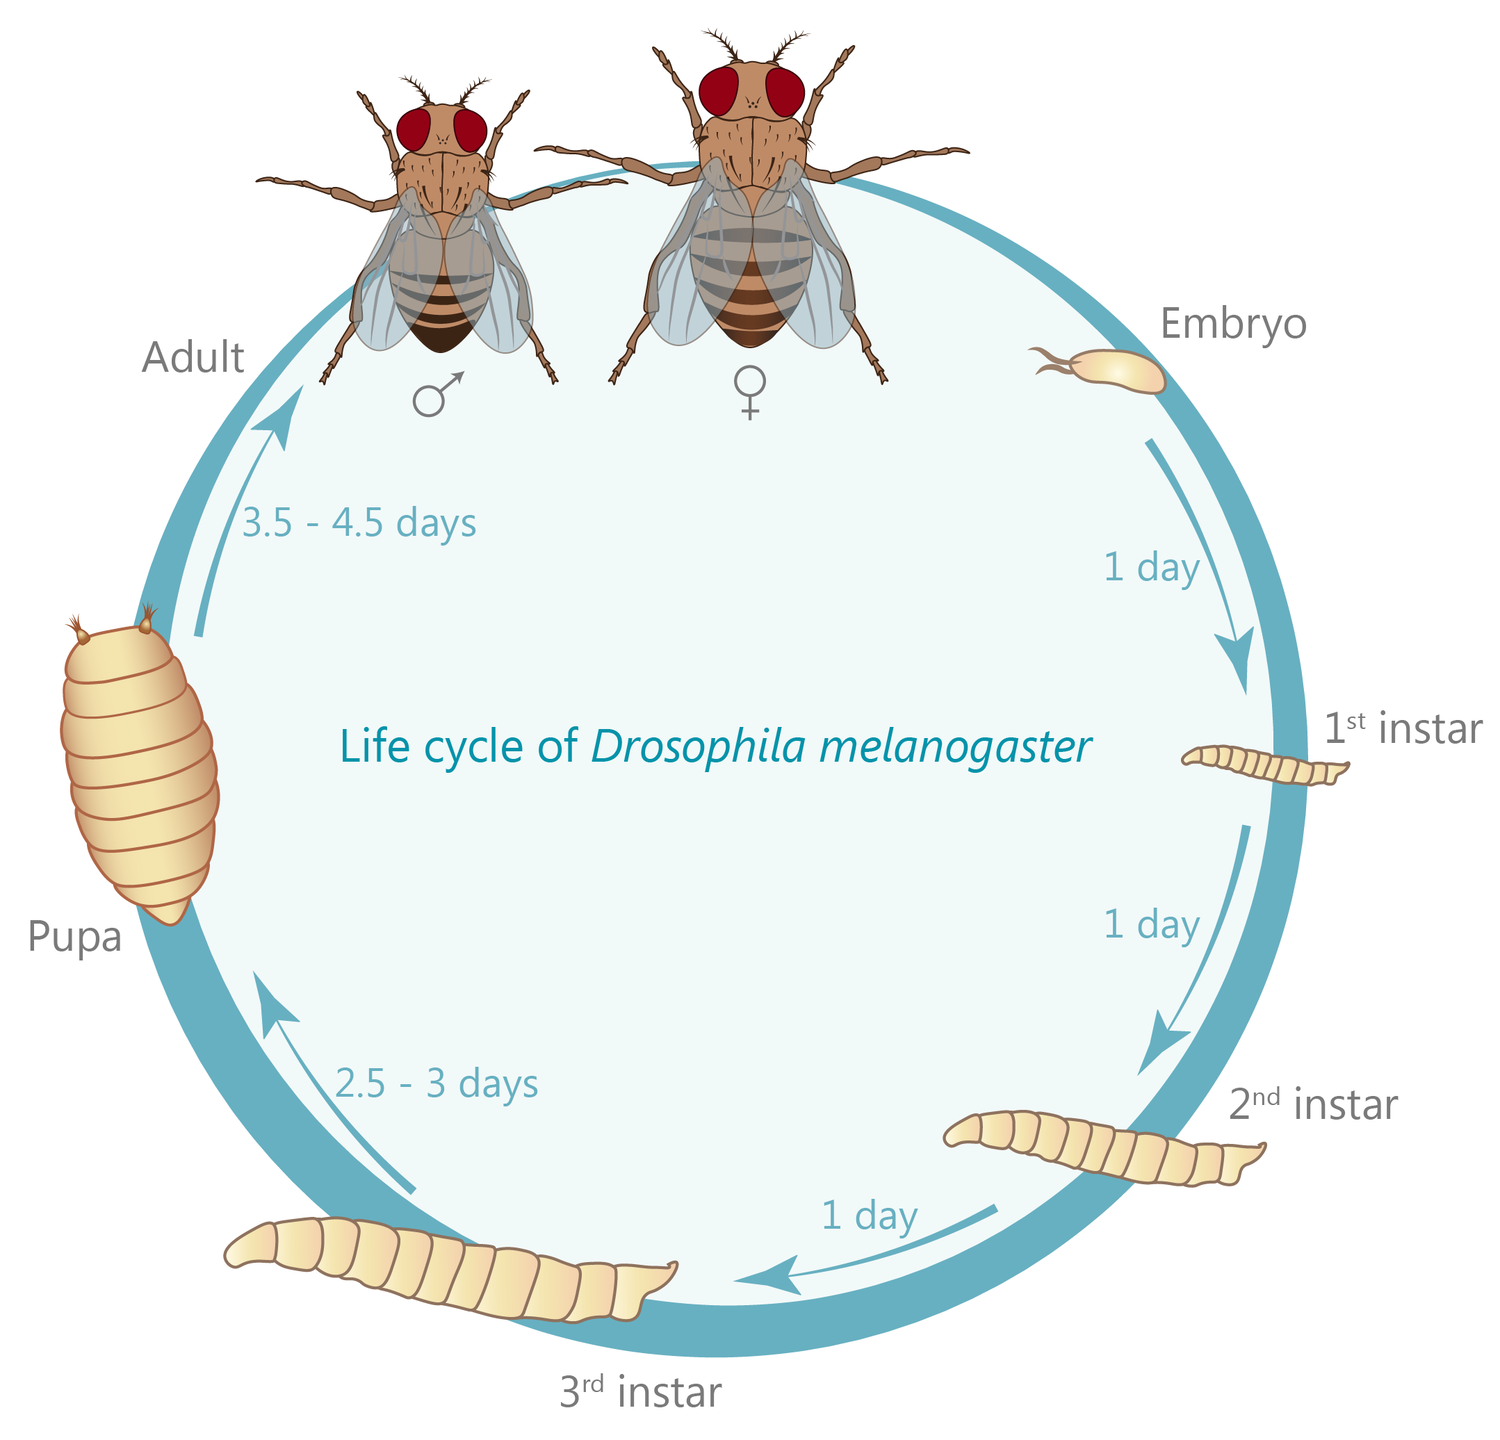
\includegraphics[width=0.7\columnwidth]{resources/model_organism_fig_1.png}
		\caption{Life \textbf{cycle} of Drosophila melanogaster. \cite{example_website}}
		\label{fig:Life_cycle_of_fruit_fly}
	\end{figure}
	
	Drosophila melanogaster undergoes a complete metamorphosis during its life cycle, which consists of four stages: egg, larva, pupa, and adult.
	
	\begin{enumerate}
		\item \textbf{Embryo}: The embryo stage is the first stage of Drosophila development. Drosophila eggs are small and oval-shaped, with a length of about 0.5 mm. They are laid singly or in clusters on moist surfaces, such as rotting fruit or moist soil. The egg contains a single cell that divides rapidly to form a multicellular embryo.
		\item \textbf{Larva}: The larva is the second stage of Drosophila development. Drosophila larvae, also known as maggots, are small, legless, and worm-like in appearance, with a length of about 5 mm. They are white or yellow in color and have a segmented body with three main regions: the head, thorax, and abdomen. The larva feeds on a variety of food sources, including rotting fruit, yeast, and other organic matter. During the larval stage, Drosophila undergoes significant changes in both form and function, including the growth of specialized organs and tissues and the development of the nervous system.
		\item \textbf{Pupa}: The pupa is the third stage of Drosophila development. Drosophila pupae are typically about the same size as the larva, but are more solid and have a more defined shape. They are typically dark in color and are enclosed in a hard, protective casing known as the puparium. During the pupal stage, Drosophila undergoes a process of metamorphosis, in which the larva transforms into the adult form. This process involves the reorganization and differentiation of tissues and organs, as well as the development of wings and other adult structures.
		\item \textbf{Adult}: The adult is the fourth and final stage of Drosophila development. Drosophila adults are small flies with a length of about 4-7 mm. They have a distinctive appearance, with a yellow or tan thorax, a black abdomen, and red eyes. Drosophila adults are sexually mature and are capable of reproducing. They feed on a variety of food sources, including fruit, nectar, and other sweet substances.
	\end{enumerate}
	
	\section{Drosophila larva as model organism}
	Drosophila larva are an important model organism in biology research due to their relatively simple nervous system, short generation time, and the availability of genetic tools for manipulating them. These characteristics make Drosophila larvae a useful tool for studying development, genetics, and neurobiology.
	
	
	\begin{enumerate}
		\item Drosophila larvae has relatively simple nervous system, which consists of about 100,000 neurons, compared to the approximately 100 billion neurons in the human brain. This simplicity makes it easier to study the development and function of the nervous system, as well as the underlying genetic and molecular mechanisms that regulate these processes.
		\item Drosophila larvae also have a short generation time, with a lifespan of about two weeks from egg to adult. This allows researchers to study development and evolution in a relatively short time frame, making Drosophila an important tool for studying the genetic basis of development and evolution.
		\item In addition, Drosophila larvae are amenable to genetic manipulation, allowing researchers to study the function of specific genes and pathways in development and behavior. For example, researchers can use techniques such as knockdown, overexpression, and gene editing to study the role of specific genes in the development and function of the nervous system.
	\end{enumerate}	
	
	These characteristics make Drosophila larvae a valuable tool for studying development, genetics, and neurobiology, and for identifying potential therapeutic targets for treating human diseases. While the brain of Drosophila larvae is certainly different from the human brain in terms of size, complexity, and overall organization, it shares many fundamental features and molecular pathways with the human brain.
	\begin{itemize}
		\item Like the human brain, the Drosophila larval brain contains various types of neurons and glial cells that perform different functions, and it is organized into distinct regions that are involved in specific behaviors and functions.
		\item Furthermore, the development and function of the Drosophila larval brain are regulated by many of the same genes and molecular pathways that regulate the development and function of the human brain. For example, many of the signaling pathways and transcription factors that regulate the development and function of the human brain are also present in the Drosophila larval brain.
	\end{itemize}
	
	Overall, studying the brain of Drosophila larvae can provide valuable insights into the fundamental processes that underlie the development and function of the nervous system, and may help to identify potential therapeutic targets for treating neurological disorders in humans.
	
	\section{Machine Learning and Deep Learning Background}
	This section discusses the concept of machine learning, as well as its subfield, deep learning, and the techniques and tools used to train models in this field. Deep learning is a type of artificial intelligence and machine learning that allows a computer to learn from experiences and perform well on new tasks, just like a human brain. This approach can be used to discover patterns and correlations through observations without human intervention and has been applied in various fields, including computer vision, speech recognition, natural language processing, and medical image processing. The following subsections provide more information on key deep learning techniques that are important to understand in the context of this thesis.
	
	\subsection{Machine Learning and types}
	Machine learning is a branch of AI that deals with improving the computer algorithms from experience and data without being explicitly programmed \cite{koza1996automated}. There	are four types of machine learning - supervised learning, unsupervised learning,semi-supervised learning, and reinforcement learning.
	In supervised learning, the algorithm or the model is trained using labeled data.
	During the training procedure, the model learns the parameters and uses these parameters to predict the outputs for unseen data. Supervised learning is of two types - regression and classification. Regression deals with continuous outputs whereas classification deals with discrete outputs. Supervised learning can be used in many applications like spam detection, object recognition, bioinformatics, etc. Though it has the above advantages, it may not generalize well to new data (overfitting), and pre-processing is a big challenge \cite{suplngdetails}.
	In unsupervised learning, the model is trained on unlabeled data to identify the
	hidden patterns and structures within the data. Unsupervised learning is also referred to as clustering. Some popular unsupervised learning algorithms are autoencoders, principal component analysis, etc. It is widely used for dimensionality reduction and exploratory analysis. The problems with unsupervised learning are that the results have high uncertainty and it is challenging to verify the outputs \cite{unsuplngdetails}.
	Semi-supervised learning is a combination of both supervised and unsupervised
	learning paradigms. The model is trained initially with the labeled data in a supervised fashion. Then unlabeled data is given to the model to predict the outputs.
	
	Later the predicted outputs are considered as the true outputs for the unlabeled data. Then the model has trained again with the combined data along with the labels. This method is helpful when we have limited labeled data. They are widely used in image and document classification tasks \cite{yoon2017semi}. Reinforcement learning works based on rewards and penalties. The goal of the model is to maximize the total reward. The model will not be given any labels, it has to figure out using trial and error approaches to come up with a solution to the problem. It gets feedback from the environment. Q-learning and Markov decision process are some of the most widely used reinforcement algorithms \cite{sutton2018reinforcement}.
	Even though machine learning algorithms have a lot of applications, they fail to perform well in image processing, natural language processing (NLP), etc. This is where deep learning is so powerful.
	
	\subsection{Deep Learning}
	Deep learning is a subset of machine learning that is inspired by the structure and function of the brain, specifically the neural networks that make up the brain. Deep learning algorithms are designed to learn and extract features from data automatically, rather than being explicitly programmed with a set of rules or features to look for.
	
	Deep learning algorithms are implemented using artificial neural networks, which are composed of multiple layers of interconnected artificial neurons, or "perceptrons." These neural networks are trained using large amounts of labeled data and a variant of the backpropagation algorithm, which adjusts the weights of the connections between the neurons based on the error between the predicted output and the actual output.
	
	Deep learning algorithms are capable of learning complex, non-linear relationships in data and have been shown to achieve state-of-the-art results in a wide variety of tasks, including image and speech recognition, natural language processing, and predictive modeling. They have been applied to a wide range of applications, including self-driving cars, medical diagnosis, and language translation.
	
	One of the key benefits of deep learning is that it can learn to extract meaningful features from raw data, without the need for manual feature engineering. This can save a lot of time and effort in the preprocessing stage of a machine learning project, and can often lead to better performance on the task at hand. However, deep learning algorithms can be computationally expensive to train and require a large amount of labeled data to be effective.
	
	\subsection{Neural Networks}
	Neural networks or artificial neural networks (ANN) are the core of deep learning
	algorithms, whose name and design are inspired by how neurons function in the
	human brain. It can learn and model non-linear and complex relationships between
	input and output. It also has the ability to generalize, which implies it can infer
	associations from unobserved data after training.
	
	Neurons or perceptrons \cite{rosenblatt1958perceptron} are the basic blocks of a neural network. A perceptron takes a set of weighted inputs, exerts an activation function, and returns an output value. \ref{fig:Single Perceptron} illustrates the model of a perceptron. It takes any number of inputs (xi), which are weighted with corresponding weights (wi) and then summed up along with a bias (b). Then the sum is subjected to an activation function ($\sigma$) to produce the final output as shown in Equation \ref{eq:perceptron}. 
	
	\begin{equation}
	y = \sigma\left(\sum\limits_{i=1}^{n} w_i x_i + b\right) \label{eq:perceptron}
	\end{equation}
	
	In this equation \ref{eq:perceptron}., y is the output of the perceptron, x\_1, x\_2, ..., x\_n are the input features, w\_1, w\_2, ..., w\_n are the weights, and b is the bias term. The sigmoid function $\sigma$(x) is defined as:
	
	\begin{equation}
	\sigma(x) = \frac{1}{1 + e^{-x}}
	\end{equation}
	
	\begin{figure}[H]
		\centering
		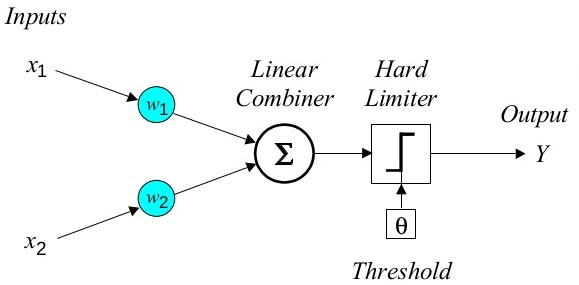
\includegraphics[scale=0.5]{resources/chapter3/perceptron.jpg}
		\caption{Illustration of model with a single perceptron. \cite{kamdem2023inputs}}
		\label{fig:Single Perceptron}
	\end{figure}
	
	Several perceptrons can be combined to solve more complex problems. Such a
	combination of neurons, which are organized in layers called multi-layer perceptrons (MLPs) as shown in \ref{fig:Multilayer Perceptron}. A multi-layered perceptron (MLP) is a type of artificial neural network that is composed of multiple layers of artificial neurons, or "perceptrons." MLPs are used for supervised learning tasks, such as classification and regression.
	
	\begin{align*}
	a_1 &= x \\
	a_2 &= f_2(w_{1,2} a_1 + b_2) \\
	a_3 &= f_3(w_{2,3} a_2 + b_3) \\
	& \ \vdots \\
	y &= f_L(w_{L-1,L} a_{L-1} + b_L)
	\end{align*}
	
	In this equation, x is the input to the neural network, a\_1, a\_2, ..., a\_L are the activations at each layer, w\_{l,l+1} are the weights between layer l and layer l+1, b\_l is the bias at layer l, and f\_l is the activation function at layer l. The output of the neural network is y.
	
	The basic structure of an MLP consists of an input layer, one or more hidden layers, and an output layer like in figure \ref{fig:Multilayer Perceptron}. The input layer receives the input data and passes it through to the hidden layers, which process the data and pass it along to the output layer. The output layer produces the final output of the MLP, which can be a classification or a prediction based on the input data.
	
	MLPs are trained using a variant of the backpropagation algorithm, which adjusts the weights of the connections between the neurons based on the error between the predicted output and the actual output. This process is repeated until the error is minimized and the MLP is able to accurately predict the output for a given input.
	
	MLPs have been widely used in many applications, including image recognition, natural language processing, and predictive modeling. However, they can be computationally expensive to train and are not well-suited to tasks that require processing large amounts of sequential data, such as language translation or speech recognition.
	
	\begin{figure}[H]
		\centering
		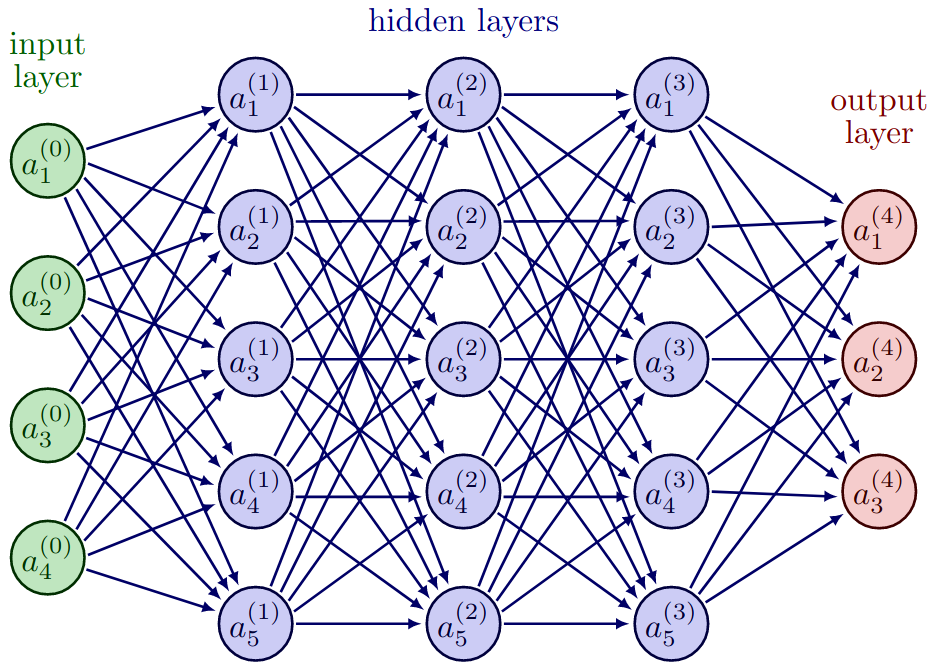
\includegraphics[width=0.7\columnwidth]{resources/chapter3/mlp.png}
		\caption{Illustration of model with a multi-layer perceptron. \cite{tikz_neural_networks}}
		\label{fig:Multilayer Perceptron}
	\end{figure}
	
	\subsection{Convolutional Neural Networks (CNNs)}
	Convolutional neural networks (CNNs) are a type of artificial neural network specifically designed for image recognition and processing. They are inspired by the structure of the visual cortex in animals, which is arranged in such a way as to be sensitive to specific patterns or features in visual stimuli.
	
	CNNs are composed of multiple layers of artificial neurons, or "perceptrons," arranged in a three-dimensional structure, with the input layer at the bottom, followed by one or more hidden layers, and an output layer at the top. The hidden layers are made up of multiple "convolutional" layers, which apply a set of learnable filters to the input data and produce a set of feature maps. These feature maps are then processed by one or more "pooling" layers, which downsample the data and reduce the spatial resolution of the feature maps. Finally, the output of the pooling layers can be passed through a fully connected layer, which produces the final output of the CNN.
	
	CNNs are trained using a variant of the backpropagation algorithm, in which the weights of the filters and connections between the neurons are adjusted based on the error between the predicted output and the actual output. This process is repeated until the error is minimized and the CNN is able to accurately classify or predict the output for a given input.
	
	\begin{figure}[h!]
		\centering
		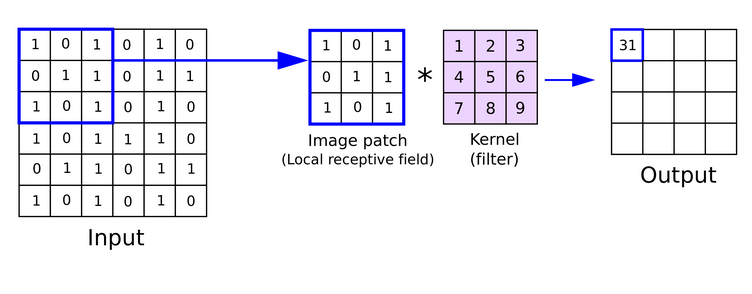
\includegraphics[width=0.7\columnwidth]{resources/chapter3/cnn2.png}
		\caption{Illustration of working of Convolutional Neural Networks (CNNs). \cite{reynolds2023convolutional}}
		\label{fig:CNN2}
	\end{figure}
	
	CNNs have achieved state-of-the-art results in many image recognition tasks and are widely used in applications such as object detection, image classification, and facial recognition.
	
	\subsection{Elements of Neural Network}
	\subsubsection{Activation function}
	
	Activation functions are used to adjust the output of each layer in a neural network. There are two types: linear and non-linear. Linear activation functions are not commonly used. Instead, non-linear activation functions are used to introduce non-linearities to the network, allowing it to learn non-linear relationships between inputs and outputs. Some common non-linear activation functions include sigmoid, tanh, ReLU, and leaky ReLU. The graphs of these activation functions are shown in Figure \ref{fig:Activation_functions} \cite{image2023, szandala2021review}.
	
	\begin{figure}[h!]
		\centering
		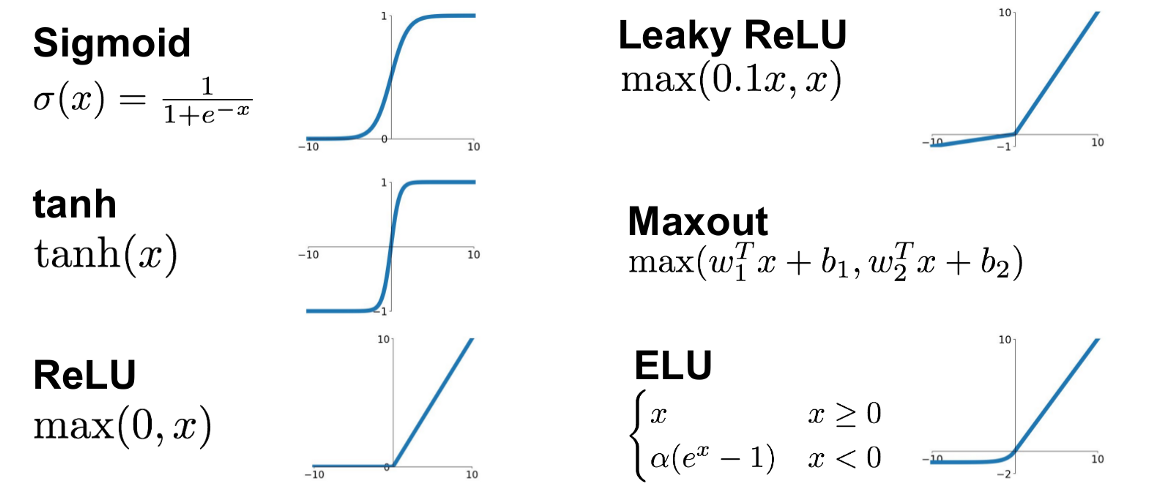
\includegraphics[width=100mm]{resources/chapter3/activation_functions.png}
		\caption{Activation functions}
		\label{fig:Activation_functions}
	\end{figure}
	
	\subsubsection{Loss function}
	
	A Loss function is used to check how our model compares to an ideal model. There are many types of loss functions, one of which can be selected based on the problem being solved. The most common ones for regression are mean absolute error (MAE) also referred to as L1 loss, mean squared error (MSE) also referred to as L2 loss. The most common ones for classification problems are binary cross-entropy (BCE) loss and hinge loss \cite{wang2020comprehensive}. And others include normalized cross correlation and mutual information loss to measure the similarity between the two images. A typical loss function plotted against the number of epochs is given in the Figure \ref{fig:LossFun} \cite{image2023mse}. 
	
	\begin{figure}[H]
		\centering
		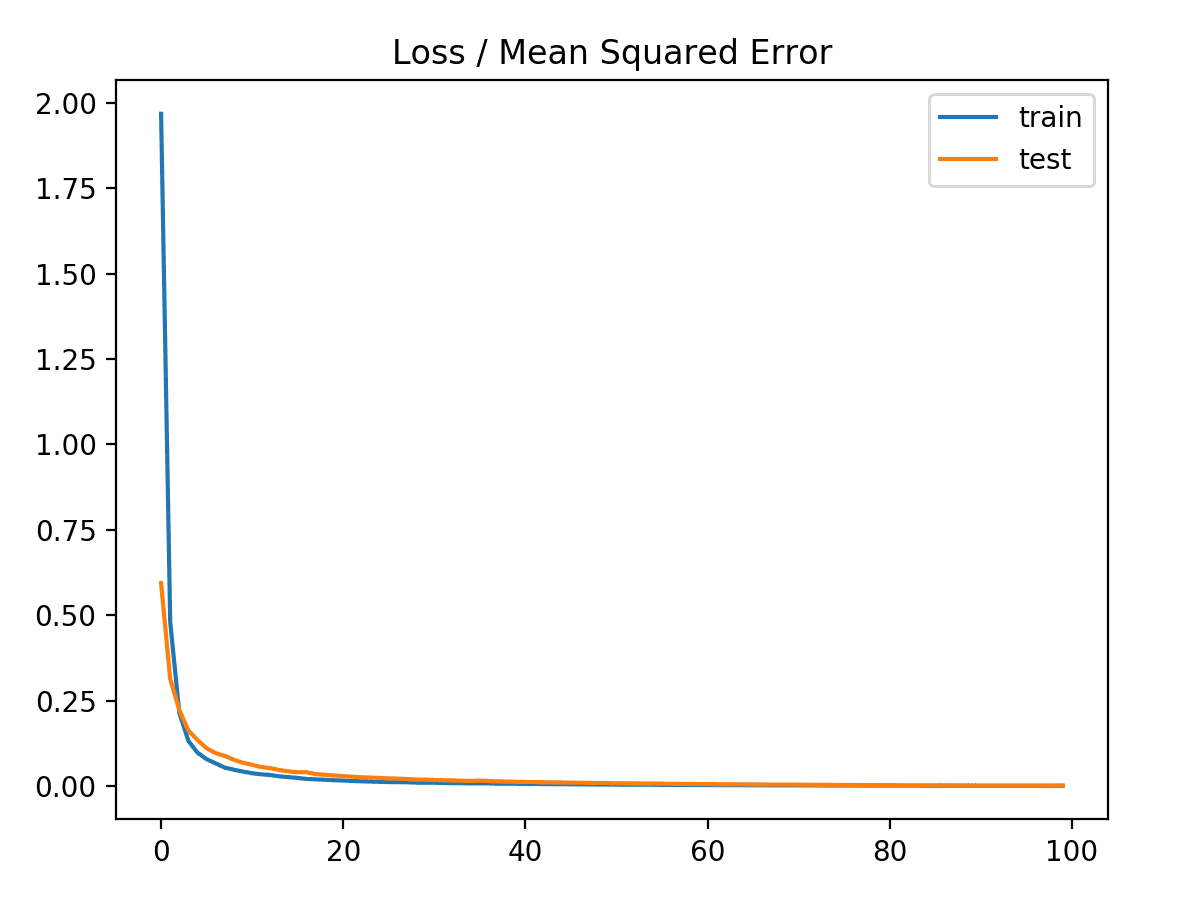
\includegraphics[scale=0.2]{resources/chapter3/lossfun.png}
		\caption{Loss function}
		\label{fig:LossFun}
	\end{figure}
	
	\subsubsection{Backpropagation}
	
	Backpropagation is an algorithm used to train artificial neural networks. It involves using gradient descent to propagate the error computed by the loss function backwards through the network. The gradients of the error with respect to the model's parameters are calculated using the chain rule of calculus, and these gradients are used to update the parameters of the model.
	
	\subsubsection{Learning rate}
	
	The learning rate is a hyperparameter that determines the size of the updates made to the model's weights during training. It is important to choose an optimal learning rate, as a value that is too small can cause the training process to be slow and potentially get stuck, while a value that is too large can cause the training process to be unstable and result in sub-optimal learned parameters. The learning rate can also be scheduled to change during the training process. \cite{senior2013empirical}. 
	
	
	\subsubsection{Optimizer}
	
	Optimizers are important in the training process of a model, as they use the gradients computed through backpropagation to update the model's parameters and minimize the loss. Some common optimizers include Adam and stochastic gradient descent. Research has shown that the Adam algorithm tends to perform well in most cases \cite{zaheer2019study}.
	
	\subsection{Encoder-Decoder Architecture}
	The encoder-decoder architecture is a type of neural network architecture commonly used in natural language processing and machine translation tasks. It consists of two main components: an encoder and a decoder.
	\begin{enumerate}
		\item The encoder takes in a sequence of input data, such as a sentence in a source language, and converts it into a fixed-length internal representation, called a "latent representation" or "latent vector." This latent vector captures the meaning of the input sequence and is typically much smaller in size than the input sequence itself.
		\item The decoder takes the latent vector as input and generates an output sequence, such as a translation of the input sentence into a target language. The decoder is typically trained to generate the output sequence by predicting the next word in the sequence based on the previous words and the latent vector.
	\end{enumerate}
	
	The encoder-decoder architecture has been widely used in natural language processing tasks, such as machine translation, language modeling, and text summarization. It has also been applied to other domains, such as image generation and sequence-to-sequence modeling in time series data.
	
	\begin{figure}[H]
		\centering
		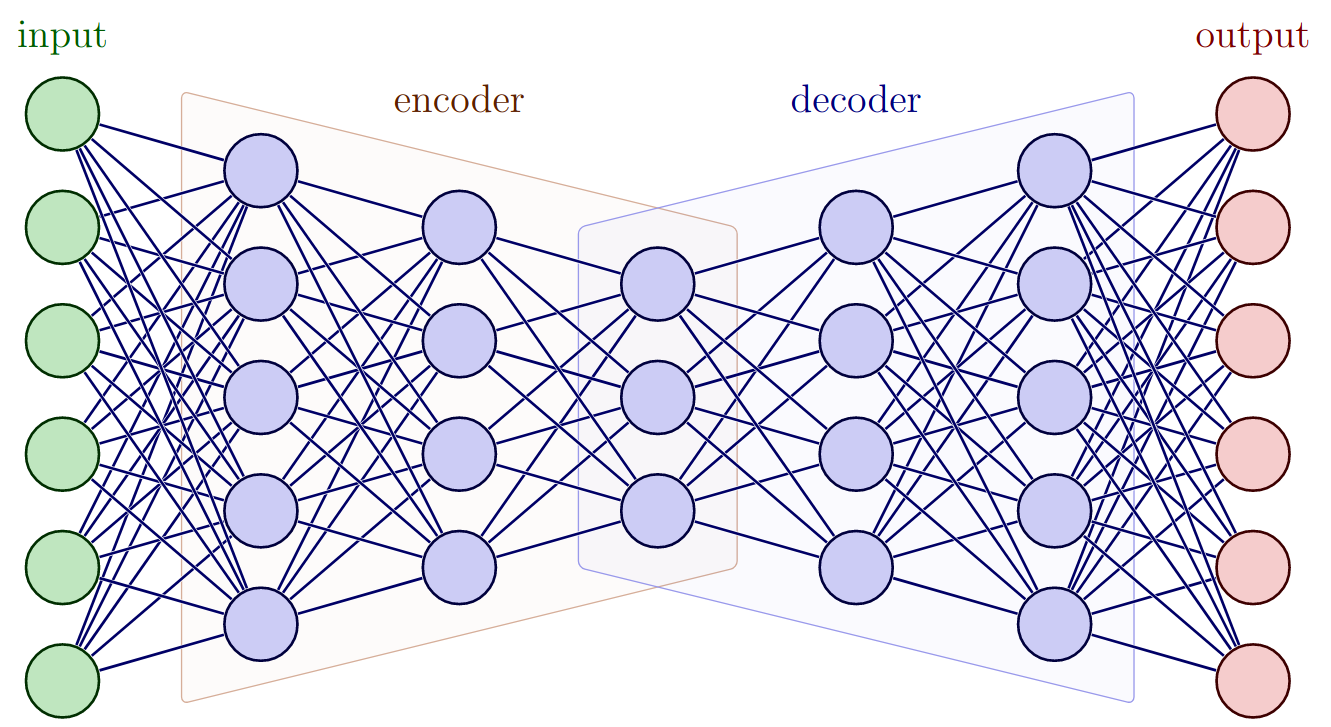
\includegraphics[width=0.7\columnwidth]{resources/chapter3/encoderdecoder.png}
		\caption{Illustration of encoder decoder architecture \cite{tikz_neural_networks}.}
		\label{fig:Encoder Decoder architecture}
	\end{figure}
	
	In image processing, the encoder-decoder architecture can be used to perform tasks such as image compression and image reconstruction.	In image compression, the encoder takes in an input image and compresses it into a smaller representation, called a "latent representation" or "latent vector" that captures the important features of the image. This latent vector captures the important features of the input image and is typically much smaller in size than the input image itself. The decoder takes the latent vector as input and reconstructs an output image that is as close as possible to the original input image.
	
	In image reconstruction tasks, the encoder-decoder architecture can be used to restore images that have been damaged or degraded in some way, such as by noise, blur, or missing pixels. It can also be used to perform tasks such as super-resolution, in which a low-resolution image is upscaled to a higher resolution.
	
	\subsection{U-Net}\label{subsec:unet}
	U-Net is a convolutional neural network (CNN) architecture designed for image segmentation tasks. It was developed by Olaf Ronneberger, Philipp Fischer, and Thomas Brox in 2015 \cite{UNet} and has since become a widely used model for image segmentation in medical imaging and other domains. U-Net is typically trained using supervised learning, with the goal of minimizing the error between the predicted output segmentation map and the ground truth segmentation map. It has been widely used in medical imaging tasks, such as tumor segmentation and organ segmentation, and has also been applied to other domains, such as satellite image analysis and surface defect detection.
	
	\begin{figure}[H]
		\centering
		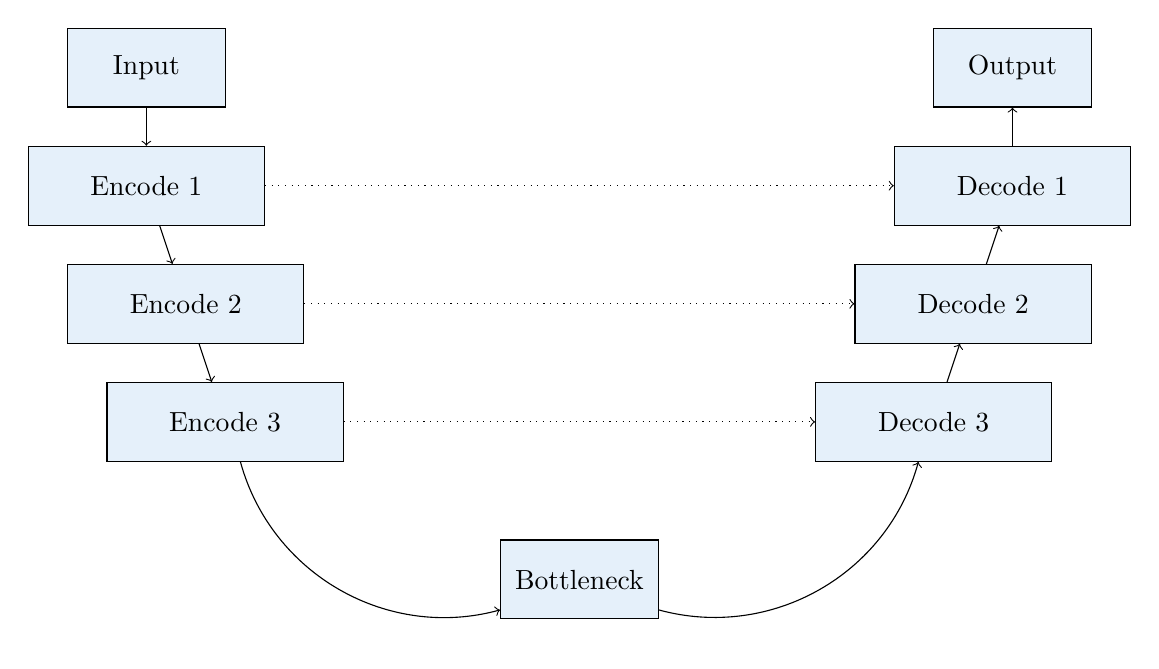
\begin{tikzpicture}[node distance=1.5cm]
		
		% Draw the input layer
		\node (input) [draw, fill=rwth-blue-5, minimum width=2cm, minimum height=1cm] {Input};
		
		% Draw the first downsampling layer
		\node (encode1) [draw, fill=rwth-blue-5, minimum width=3cm, minimum height=1cm, below of=input] {Encode 1};
		
		% Draw the second downsampling layer
		\node (encode2) [draw, fill=rwth-blue-5, minimum width=3cm, minimum height=1cm, below of=encode1, xshift=0.5cm] {Encode 2};
		
		% Draw the third downsampling layer
		\node (encode3) [draw, fill=rwth-blue-5, minimum width=3cm, minimum height=1cm, below of=encode2, xshift=0.5cm] {Encode 3};
		
		% Draw the first bottleneck layer
		\node (bottleneck) [draw, fill=rwth-blue-5, minimum width=2cm, minimum height=1cm, right of=encode3, xshift=3cm, yshift=-2cm] {Bottleneck};
		
		% Draw the upsampling layers
		\node (decode3) [draw, fill=rwth-blue-5, minimum width=3cm, minimum height=1cm, right of=bottleneck, xshift=3cm, yshift=2cm] {Decode 3};
		\node (decode2) [draw, fill=rwth-blue-5, minimum width=3cm, minimum height=1cm, above of=decode3, xshift=0.5cm] {Decode 2};
		\node (decode1) [draw, fill=rwth-blue-5, minimum width=3cm, minimum height=1cm, above of=decode2, xshift=0.5cm] {Decode 1};
		
		% Draw the output layer
		\node (output) [draw, fill=rwth-blue-5, minimum width=2cm, minimum height=1cm, above of=decode1] {Output};
		
		% Connect the layers with arrows
		\draw[->] (input) -- (encode1);
		\draw[->] (encode1) -- (encode2);
		\draw[->] (encode2) -- (encode3);
		\draw[->] (encode3) to[bend right=45] (bottleneck);
		\draw[->] (bottleneck) to[bend right=45] (decode3);
		\draw[->] (decode3) -- (decode2);
		\draw[->] (decode2) -- (decode1);
		\draw[->] (decode1) -- (output);
		
		% Add skip connections
		\draw[dotted,->] (encode1) -- (decode1);
		\draw[dotted,->] (encode2) -- (decode2);
		\draw[dotted,->] (encode3) -- (decode3);	
		\end{tikzpicture}
		\caption{A graphical representation of the U-Net model.}
		\label{fig:unet_tikzpicture}
	\end{figure}
	Figure~\ref{fig:unet_tikzpicture} shows the structure of the U-Net model. The model has two main parts: an encoder that reduces the spatial resolution of the input image and increases the number of feature maps, and a decoder that does the opposite. The encoder uses convolutional layers with a stride of 2 to downsample the input image, and the decoder uses transposed convolutional layers to upsample the feature maps. The bottleneck layer connects the encoder and decoder and acts as a bridge between them. It allows the decoder to use the high-level features extracted by the encoder to generate a detailed segmentation map. The model also has skip connections, shown as dotted lines in the figure, that allow the decoder to access the features extracted by the encoder at each level of the network. This helps the model to use both high-level and low-level features and preserves spatial information, leading to more accurate segmentation results.
	
	The input to the model is an image and the output is a segmentation mask, with each pixel in the mask corresponding to a particular class in the image. The U-Net model is commonly used in medical imaging, where it can be trained to segment organs or other structures in images.
	
	\section{Loss Metric}\label{sec:loss_metric}
	A loss metric, also known as a loss function or objective function, is a measure of how well a machine learning model is able to predict the correct output for a given input. It is used to evaluate the performance of the model during training and to guide the optimization process.
	
	There are many different loss functions that can be used, depending on the specific task being addressed and the characteristics of the data. Some common loss functions that are used in image registration include:
	
	\begin{enumerate}
		\item \textbf{Mean squared error (MSE)}
		\item \textbf{Normalized cross-correlation (NCC)}
		\item \textbf{Landmark registration error}
	\end{enumerate}
	
	\subsection{Mean squared error (MSE)}
	This is a common loss function that measures the average squared difference between the predicted output and the true output. It is often used for regression tasks and is particularly useful for image registration because it is sensitive to small errors and can effectively penalize large errors.
	
	The mean squared error (MSE) between two images, fixed image $I_f$ and moved image $I_m$, can be calculated as:
	
	$$ MSE = \frac{1}{n} \sum_{i=1}^n (I_f(i) - I_m(i))^2 $$
	
	where $n$ is the number of pixels in the images and $I_f(i)$ and $I_m(i)$ represent the intensity values of the fixed and moved images at pixel $i$, respectively.
	
	\subsection{Normalized cross-correlation (NCC)}
	This loss function measures the similarity between two images by calculating the cross-correlation between them and normalizing by the product of their standard deviations. It is commonly used in image registration because it is robust to intensity variations and can handle images with different scales or contrast.
	
	
	The normalized cross-correlation (NCC) between two images, fixed image $I_f$ and moved image $I_m$, can be calculated as:
	
	$$ NCC = \frac{\sum_{i=1}^n (I_f(i) - \mu_f)(I_m(i) - \mu_m)}{\sqrt{\sum_{i=1}^n (I_f(i) - \mu_f)^2}\sqrt{\sum_{i=1}^n (I_m(i) - \mu_m)^2}} $$
	
	where $n$ is the number of pixels in the images, $I_f(i)$ and $I_m(i)$ represent the intensity values of the fixed and moved images at pixel $i$, respectively, and $\mu_f$ and $\mu_m$ are the mean intensities of the fixed and moved images, respectively.
	
	\subsection{Landmark registration error}
	This loss function measures the error between the predicted and true locations of landmarks in the images being registered. It is often used in conjunction with other loss functions to guide the optimization process and ensure that the images are correctly aligned.
	
	The landmark registration error between two images, fixed image $I_f$ and moved image $I_m$, can be calculated as the mean Euclidean distance between corresponding landmarks in the two images:
	
	$$ LRE = \frac{1}{K} \sum_{k=1}^K \sqrt{(x_f^k - x_m^k)^2 + (y_f^k - y_m^k)^2 + (z_f^k - z_m^k)^2} $$
	
	where $K$ is the number of landmarks, $(x_f^k, y_f^k, z_f^k)$ and $(x_m^k, y_m^k, z_m^k)$ represent the coordinates of the $k$-th landmark in the fixed and moved images, respectively.
	
	\section{Quality Assessment}\label{sec:quality}
	It is important to evaluate the performance of an image registration method using multiple metrics because the loss function, such as normalized cross-correlation error (NCC) or mean squared error (MSE), only measures the overall error in the registration. These metrics do not necessarily capture errors that occur at specific, biologically significant local regions. Therefore, evaluating the performance qualitatively and quantitatively becomes necessary help to identify and quantify errors at such local regions. This can provide a more comprehensive assessment of the accuracy and effectiveness of the image registration method.
	
	\subsection{Quantitative Assessment}
	Quantitative assessment metrics are numerical measures that are used to evaluate the performance. The specific metric used will depend on the characteristics of the data and the goals of the analysis. In our image registration task, in addition to optimizing the loss function, such as normalized cross-correlation error (NCC), we  evaluate below metrics to assess the performance of our approach.
	\begin{enumerate}
		\item \textbf{Ventricular Error Indicator (VI)}
		\item \textbf{Thoracic Nerve Entry Error Indicator (TI)}
		\item \textbf{Landmark registration error (LRE)}
	\end{enumerate}
	
	
	\subsubsection{Ventricular Error Indicator (VI)}
	To evaluate the accuracy of the image registration in the Ventricular Nerve Cord (VNC) region, we consider 2 small 3D spherical volumes in the VNC entry points in both the fixed and moved images and compute the mutual information between these regions. A high score indicates that the image registration is good, while a low score indicates that there are errors in the registration. With this score, we can determine the quality of the image registration at this locality.
	
	\subsubsection{Thoracic Nerve Entry Error Indicator (TI)}
	To evaluate the accuracy of the image registration at thoracic nerve entry, we consider 6 small 3D spherical volumes around the 6 thoracic nerve entry points in both the fixed and moved images and compute the mutual information between these regions. A high score indicates that the image registration is good, while a low score indicates that there are errors in the registration. With this score, we can determine the quality of the image registration at this locality.
	
	\subsubsection{Landmark registration error (LRE)}
	In the larvalign paper, biologists identified 30 distinct and biologically significant points in the brain scan of a drosophila larva that can be used as landmarks. We use the same landmarks in this study also. Landmark registration error (LRE) is a measure of the accuracy of the alignment of the landmarks in two images, and is commonly used in medical imaging and other fields where the alignment of specific features or structures is important. A low LRE score indicates that the image registration is accurate, while a high score indicates that there are errors in the alignment of the landmarks. By comparing the LRE scores, we can determine the quality of the image registration at these landmark sites.
	
	\subsection{Qualitative Assessment}
	While quantitative assessments involve the use of numerical measurements and statistical analysis to objectively assess the performance or quality of something. The qualitative assessments involve the use of subjective observations and interpretations to evaluate the performance or quality of something. These methods are often preferred because they can provide insights and understanding that may not be captured by quantitative methods, and they can be used to identify trends and patterns that may not be immediately apparent from numerical data alone.
	For this purpose, we use the \texttt{imshowpair} function in MATLAB to overlay the fixed image and the registered image. The resulting image will show the original intensity values where the two images perfectly overlap, and it will show green or magenta values in areas where there is no overlap. This allows us to visually inspect the registration and identify any discrepancies.
	
	\chapter{Methods and Implementations}
	In Chapter \ref{chap:litreture}, we reviewed various traditional and deep learning approaches for medical image registration. In this chapter, we will delve into the specific methods we selected for our study and explain why they were chosen and how they are effective in addressing the challenges of medical image registration.
	
	In the following three sections, we will address the specifics of the Voxelmorph architecture \cite{Balakrishnan_2019} that served as the foundation for our study, explore the concept of landmark points and their importance in the field of image registration, and provide an overview of the dataset we used and the preprocessing steps we applied to it in order to prepare it for analysis.
	
	\section{The Voxelmorph Architecture: An Overview}
	\label{sec:vxm_architecture}
	
	In the paper, "VoxelMorph: a learning framework for deformable medical image registration," \cite{Balakrishnan_2019} the authors introduce a deep learning architecture called Voxelmorph for medical image registration. The architecture of Voxelmorph is designed specifically for medical image registration, which is the process of aligning two or more medical images of the same subject, taken at different times or using different modalities, in order to compare and analyze them.
	
	The Voxelmorph architecture consists of two main components: an encoder-decoder CNN architecture (U-Net) \cite{UNet} and a spatial transformer network (STN) \cite{NIPS2015_33ceb07b}. The U-Net is responsible for learning the spatial transformations needed to align the images, while the spatial transformer network is responsible for applying those transformations to the images.
	
	In the Voxelmorph architecture, the U-Net is modified to predict a dense displacement field, which describes how the pixels in the target image should be displaced in order to align with the source image. The displacement field is then passed through spatial transformer network (STN), which uses it to warp the moving image and bring it into alignment with the fixed image. The U-Net architecture is particularly well-suited for this task because it is able to capture both high-level semantic features and fine-grained spatial details in the input images.
	
	\begin{figure}[h!]
		\centering
		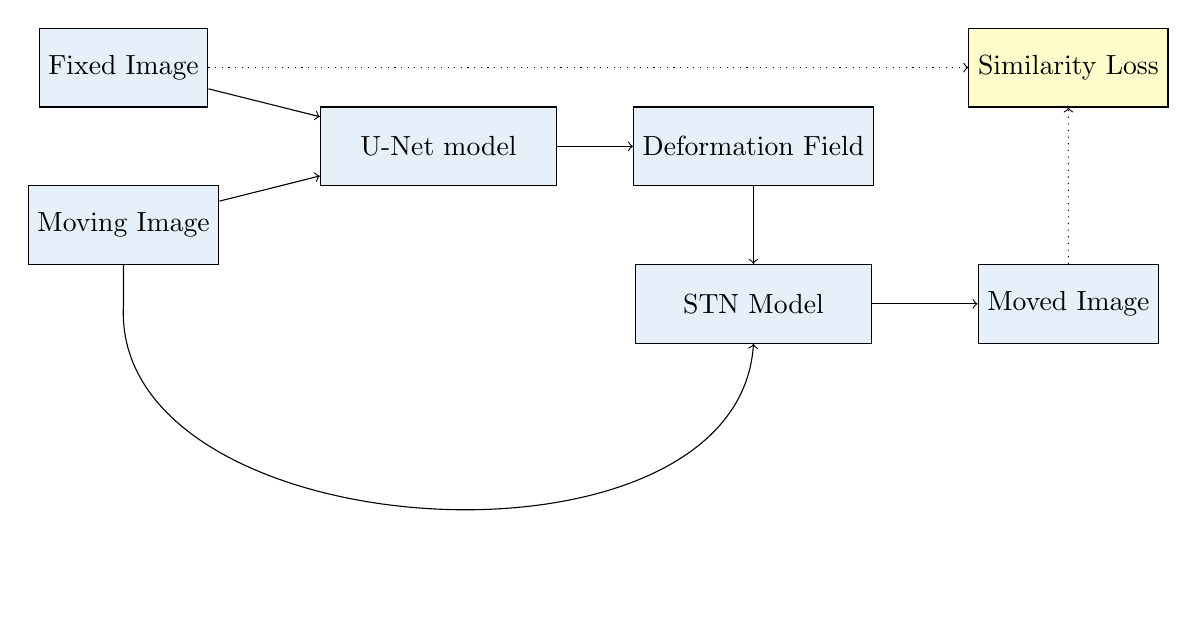
\begin{tikzpicture}[node distance=2cm]
		% Draw the input layer
		\node (fixed) [draw, fill=rwth-blue-5, minimum width=2cm, minimum height=1cm] {Fixed Image};
		\node (moving) [draw, fill=rwth-blue-5, minimum width=2cm, minimum height=1cm, below of=fixed] {Moving Image};
		
		% Draw the U-Net model
		\node (unet) [draw, fill=rwth-blue-5, minimum width=3cm, minimum height=1cm, right of=fixed, xshift=2cm, yshift=-1cm] {U-Net model};
		
		% Draw the output of the U-Net model
		\node (deformation) [draw, fill=rwth-blue-5, minimum width=2cm, minimum height=1cm, right of=unet, xshift=2cm] {Deformation Field};
		
		% Draw the STN model
		\node (stn) [draw, fill=rwth-blue-5, minimum width=3cm, minimum height=1cm, below of=deformation] {STN Model};
		
		% Draw the output of the STN model
		\node (moved) [draw, fill=rwth-blue-5, minimum width=2cm, minimum height=1cm, right of=stn, xshift=2cm] {Moved Image};
		
		% Draw the similarity loss block
		\node (loss) [draw, fill=yellow!20, minimum width=2cm, minimum height=1cm, right of=fixed, xshift=10cm] {Similarity Loss};
		
		% Connect the layers with arrows
		\draw[->] (fixed) -- (unet);
		\draw[->] (moving) -- (unet);
		\draw[->] (unet) -- (deformation);
		\draw[->] (deformation) -- (stn);
		\draw[->] (moving) -- (moving |- stn) to[bend right=90] (stn);
		\draw[->] (stn) -- (moved);
		
		% Draw the arrows between the blocks
		\draw[dotted, ->] (fixed) -- (loss);
		\draw[dotted, ->] (moved) -- (loss);	
		\end{tikzpicture}
		\caption{A graphical representation of the Voxelmorph model where the U-Net model takes as input the fixed image and the moving image, and produces a deformation field as output.}
		\label{fig:vxm_tikzpicture}
	\end{figure}
	
	The basic structure of Voxelmorph consists of an encoder-decoder architecture (U-Net) with skip connections between the encoder and decoder layers as illustrated in Subsection~\ref{subsec:unet}. The encoder takes in a pair of input images and extracts features from them, while the decoder generates a dense displacement field that maps pixels from one image to the other. The skip connections allow the decoder to access the features extracted by the encoder at each level of the network, which helps to preserve spatial information and improve the accuracy of the displacement field.
	
	The figure \ref{fig:vxm_tikzpicture} is an illustration of the Voxelmorph model. The model consists of two main components: a U-Net model and an STN model. The U-Net model takes as input the fixed image and the moving image, and produces a deformation field as output. The STN model, or spatial transformer network model, takes as input the deformation field and the moving image, and produces a moved image as output. The STN model is responsible for applying the deformation field to the moving image, effectively aligning it with the fixed image. The moved image is then compared to the fixed image using a similarity loss function, which is represented by the block labeled "Similarity Loss" in the illustration. The dotted arrows in the illustration indicate that the similarity loss is calculated between the fixed image and the moved image. The model is trained to minimize the similarity loss, which helps to align the moving image with the fixed image.
	
	Figure~\ref{fig:vxmaux_tikzpicture} depicts a model that includes an auxiliary information block in addition to the fixed and moving images as input to the U-Net model. This auxiliary information can improve the accuracy of the deformation field produced by the U-Net model. Researchers have found that using segmentation masks as auxiliary input can enhance the model's performance on specific tasks. For example, segmentation masks can help the model focus on specific areas of the image, such as the brain or heart, and improve the accuracy of the displacement field in those areas.
	
	The Voxelmorph architecture is designed to be fast and accurate, and it has been widely used in the field of medical image analysis since its introduction. Considering its impressive performance and widespread adoption in the field of medical image analysis, we determined that the Voxelmorph architecture was the best choice for our research and therefore used it as the base architecture.
	
	\begin{figure}[h!]
		\centering
		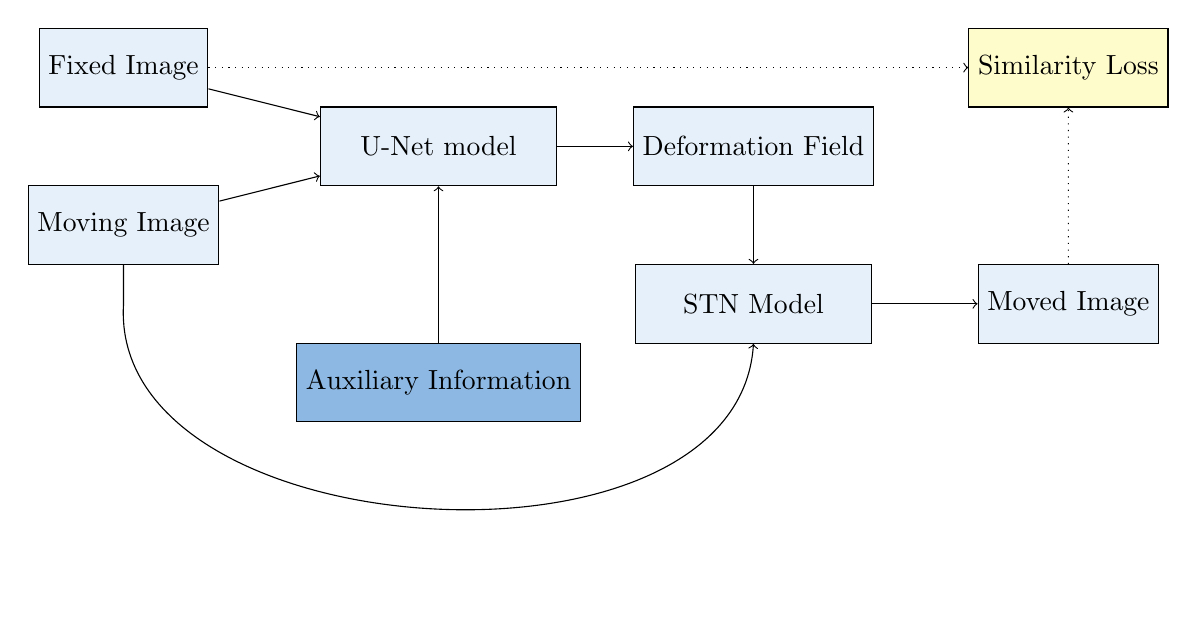
\begin{tikzpicture}[node distance=2cm]
		% Draw the input layer
		\node (fixed) [draw, fill=rwth-blue-5, minimum width=2cm, minimum height=1cm] {Fixed Image};
		\node (moving) [draw, fill=rwth-blue-5, minimum width=2cm, minimum height=1cm, below of=fixed] {Moving Image};
		
		% Draw the U-Net model
		\node (unet) [draw, fill=rwth-blue-5, minimum width=3cm, minimum height=1cm, right of=fixed, xshift=2cm, yshift=-1cm] {U-Net model};
		
		% Draw the aux
		\node (auxinfo) [draw, fill=rwth-blue-3, minimum width=2cm, minimum height=1cm, below of=unet, yshift=-1cm] {Auxiliary Information};
		
		% Draw the output of the U-Net model
		\node (deformation) [draw, fill=rwth-blue-5, minimum width=2cm, minimum height=1cm, right of=unet, xshift=2cm] {Deformation Field};
		
		% Draw the STN model
		\node (stn) [draw, fill=rwth-blue-5, minimum width=3cm, minimum height=1cm, below of=deformation] {STN Model};
		
		% Draw the output of the STN model
		\node (moved) [draw, fill=rwth-blue-5, minimum width=2cm, minimum height=1cm, right of=stn, xshift=2cm] {Moved Image};
		
		% Draw the similarity loss block
		\node (loss) [draw, fill=yellow!20, minimum width=2cm, minimum height=1cm, right of=fixed, xshift=10cm] {Similarity Loss};
		
		% Connect the layers with arrows
		\draw[->] (fixed) -- (unet);
		\draw[->] (moving) -- (unet);
		\draw[->] (unet) -- (deformation);
		\draw[->] (auxinfo) -- (unet);
		\draw[->] (deformation) -- (stn);
		\draw[->] (moving) -- (moving |- stn) to[bend right=90] (stn);
		\draw[->] (stn) -- (moved);
		
		% Draw the arrows between the blocks
		\draw[dotted, ->] (fixed) -- (loss);
		\draw[dotted, ->] (moved) -- (loss);	
		\end{tikzpicture}
		\caption{A graphical representation of the Voxelmorph model with auxiliary information where the auxiliary information in addition to the fixed and moving images are provided as input to the U-Net model.}
		\label{fig:vxmaux_tikzpicture}
	\end{figure}
	
	\section{Landmark Points: A Key Element in Image Registration} \label{sec:landmark_points}
	Landmark points in image registration, also known as fiducial points, are points of reference in an image that are used to align or register two or more images. These points are often selected based on their distinct and easily identifiable features, and are used to establish a common coordinate system for the images being registered.
	
	The term "gold standard" refers to the fact that these points are considered to be the most accurate and reliable points of reference for aligning images. This term is used metaphorically, as gold is often considered a symbol of excellence and high quality. In the context of image registration, the use of landmark points as the gold standard for alignment helps to ensure the accuracy and reliability of the registration process.
	
	In a research paper on \textit{larvalign} \cite{larvalign}, biologists have identified 30 potential landmark locations in brain scans of drosophila larva. These landmarks are also used in this thesis.
	
	\begin{figure}[h!]
		\centering
		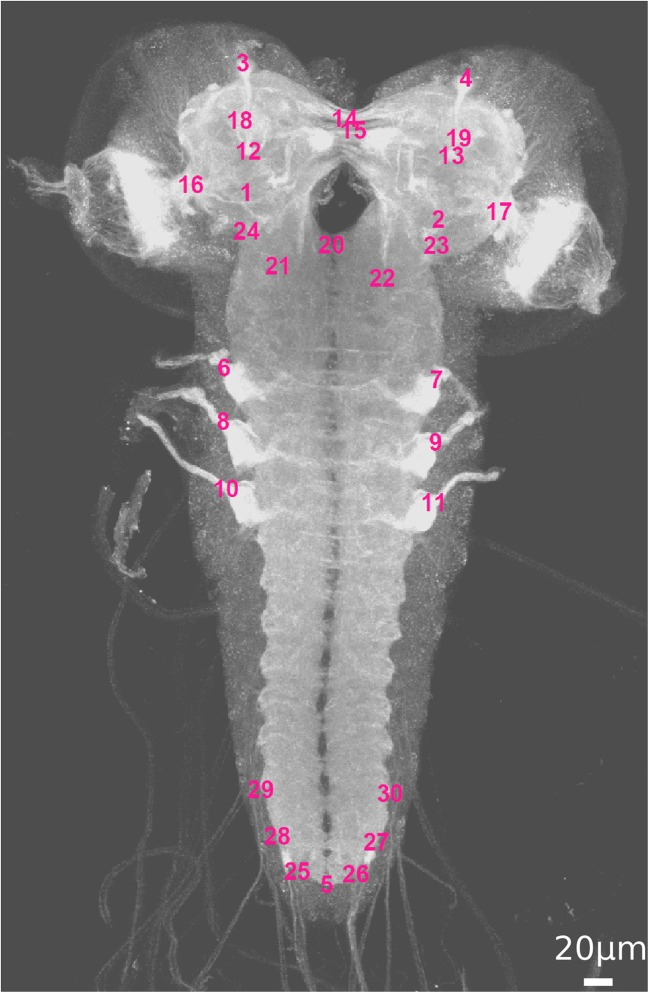
\includegraphics[width=0.5\columnwidth]{resources/chapter3/landmarks.jpg}
		\caption{Maximum intensity projection (MIP) of an example scan with annotated landmarks \cite{larvalign}.}
		\label{fig:landmark_annotations}
	\end{figure}
	
	To annotate or label these landmark points in the brain scan images, we can use ImageJ software. ImageJ is an open-source image processing software that offers "Point Tool" to label the landmark points. The "Point Tool" allows you to place a single point on an image by clicking on the desired location.
	
	To use the "Point Tool" in ImageJ Fiji for landmark annotation, follow these steps:
	\begin{enumerate}
		\item Open the image you want to annotate in ImageJ Fiji.
		\item Click on the "Point Tool" icon in the toolbar at the top of the window. This will activate the tool and allow you to place points on the image.
		\item Click on the location in the image where you want to place a point. A small crosshair will appear at the location you clicked.
		\item Use the "Set/Add Point" button to label the point with a name or identifier. You can enter the name in the text field that appears and then click "OK" to set the name for the point.
		\item Repeat steps 3 and 4 for each additional point you want to place on the image.
		\item When you are finished annotating the points, you can use the "Point Tool" icon again to deactivate the tool and return to the default cursor.
	\end{enumerate}

	When you use the "Point Tool" to annotate an image in ImageJ, the result of the annotation will be saved in the same directory as the image as an XML file with a ".points" extension. This file will contain the coordinates of the points that you added to the image, as well as any other information about the points (such as labels and attributes).
	
	\section{Data Preparation: Selecting and Preprocessing Datasets}
	This section covers the selection and preparation of datasets for use with the Voxelmorph model. It will cover how to categorize the datasets for training and testing, as well as the necessary preprocessing steps to ensure that the data is properly formatted for the model.
	
	\subsection{Dataset}
	For this research, we have obtained three datasets from different sources: the \texttt{Leipzig dataset} from the University of Leipzig in Germany, the \texttt{Janelia dataset} from the Janelia Research Campus in Virginia, and the \texttt{Larvalign dataset} from the \textit{Larvalign} research paper \cite{larvalign}. These datasets will be referred to by these names throughout the study.
	
	As shown in Table~\ref{tab:mytable}, the datasets for this study were divided into three categories by the biologists: good quality, medium quality, and random quality. This separation was necessary to ensure that the training data was balanced and to allow us to evaluate the model's performance on different quality levels of the images.
	
	% Please add the following required packages to your document preamble:
	\begin{table}[h!]
		\centering
		\resizebox{\textwidth}{!}{%
			\begin{tabular}{|l|l|c|c|c|}
				\hline
				& Quality & Number of Scans & Original Resolution & Scaled Resolution           \\ \hline
				\multirow{3}{*}{\texttt{Leipzig dataset}}& & 100             & 980x1440x81         & \multirow{9}{*}{256x512x64} \\ \cline{2-3}
				& & 052              & 512x512x104         &                             \\ \cline{2-3}
				& & 200             & 592x800x102         &                             \\ \cline{1-3}
				\multirow{3}{*}{\texttt{Janelia dataset}}                      & Medium & 200             & 977x1428x76         &                             \\ \cline{2-3}
				& Good & 200             & 981x1428x76         &                             \\ \cline{2-3}
				& Random & 200             & 973x1434x79         &                             \\ \cline{1-3}
				\multirow{3}{*}{\texttt{Larvalign dataset (Test Data)}}                        & Medium & 021              & 973x1434x79         &                             \\ \cline{2-3}
				& Good & 020              & 981x1430x79         &                             \\ \cline{2-3}
				& Random & 025              & 977x1432x77         &                             \\ \hline
			\end{tabular}
		}
		\caption{Dataset distribution.}
		\label{tab:mytable}
	\end{table}
	
	One issue that was encountered during the data preparation process was that the images were of different sizes and resolutions. To input the images into the network, they had to be resized to a consistent size. However, the Voxelmorph model was computationally intensive and required a significant amount of memory due to the various levels of encoding and the need to retain encoded feature maps for later use in the decoding stage through skip connections. Experiments showed that using the model with images that were \texttt{256x512x64} in size required at least a \texttt{16GB GPU}. If the image volumes were larger than this resolution, a GPU with a memory capacity proportional to the expansion of the input images was required. Empirically, it was found that the GPU memory requirement was directly proportional to the increase in image volume by more than 1. As a result, it was decided to use scaled-down resolution images of \texttt{256x512x64} for all experiments. Unless stated otherwise, all experiments from that point forward were based on images with this resolution. The scaling down operation was performed by resampling the image using the bicubic interpolation algorithm present in the ImageJ Fiji tool.
	
	\subsection{Affine registration}
	According to the Voxelmorph research paper \cite{Balakrishnan_2019}, it was recommended to perform affine alignment on the input images before using them with the Voxelmorph model for deformable registration. This preprocessing step could improve the performance of the model compared to using the images without affine alignment.
	
	Similar to Voxelmorph, the \textit{larvalign} software \cite{larvalign} also performed affine alignment and then applied non-rigid registration to the affine-aligned image. Therefore, to compare the efficiency of non-rigid registration using \textit{larvalign} versus a deep learning method, it was decided to use \textit{larvalign} to perform affine registration on the input images so that both approaches would be working with the same pre-processed data. This allowed for a fair comparison of the two approaches.
	
	\begin{tcolorbox}[colback=rwth-blue-5,colframe=rwth-blue-1,title=\textbf{Larvalign Software}]
		Larvalign is based on the Elastix Registration Toolbox, which is a widely used, open-source medical image registration toolbox that allows for both rigid and non-rigid registration of medical images such as CT, MRI, and PET scans.
		\tcblower
		Elastix uses optimization algorithms to minimize a cost function that measures the difference between the images and finds the transformation that best aligns them. It offers a range of customization options, including the choice of optimization algorithm, cost function, and regularization terms, as well as pre-processing and post-processing tools to improve the accuracy and efficiency of the registration.
	\end{tcolorbox}
	
	The figure below illustrates an example of an image before and after affine alignment.
	
	\begin{figure}[H]
		\centering
		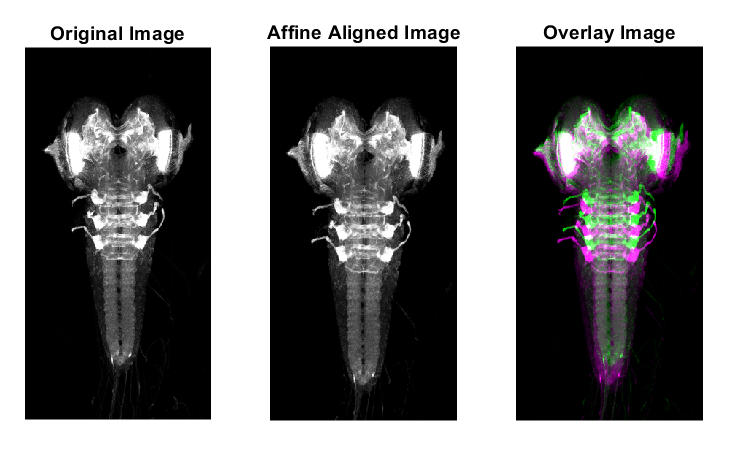
\includegraphics[width=0.9\columnwidth]{resources/chapter3/np_58E02_37E10_MB299C_021713A_scaled.tif.png}
		\caption{Affine registration example against the \textit{larvalign} template \cite{larvalign}.}
		\label{fig:affine_larvalign}
	\end{figure}

	Affine alignment is a method for aligning two images by applying an affine transformation to one of the images. An affine transformation can include rotation, scaling, translation, and shearing, and it can be used to match corresponding points in the two images. It is possible that the scale of the moving image could be changed during affine registration to match the scale of the fixed image so that moving image is aligned as much as possible with the fixed image. In the Figure~\ref{fig:affine_larvalign}, the affine registration is performed against the \textit{larvalign} template (shown in Figure~\ref{fig:Registration}), and the resulting alignment is shown before and after registration in the left and center images, respectively. The right image shows an overlay of the two images, before and after registration.
	
	\subsection{Background Noise Removal and Normalizing}
	\subsubsection{Background Noise Removal}
	To prepare the image for further processing, the noise in the background was removed by clipping the intensity values of the pixels between the mean intensity of the image and the maximum intensity (\texttt{255 for an 8-bit image}). Any values that are below the mean intensity are set to zero, while values above the mean intensity are retained. This helped to clean up the image and reduce the impact of noise on subsequent steps.
	
	The below pseudo code defines a function called \texttt{cleanup\_background} that takes an image as input and returns a modified version of the image with the background pixels set to zero.
	
	\begin{lstlisting}[language=python, label=lst:bgcorrection]

	def cleanup_background(image):
		# Find the mean intensity of the image
		mean_intensity = find_mean_intensity(image)
	
		# Set the low and high values for clipping
		low = mean_intensity
		high = 255
	
		# Clip the pixel intensity values between the low and high values
		image = clip_intensity_values(image, low, high)
	
		# Set the low clipped values to zero
		image = set_low_values_to_zero(image, low)
	
		return image
	
	\end{lstlisting}	
	
	The function shown in the Listing~\ref{lst:bgcorrection} performs the following steps:
	
	\begin{enumerate}
		\item It calls a function called \texttt{find\_mean\_intensity} to calculate the mean intensity of the image.
		\item It sets the low and high values for clipping to the mean intensity and the maximum intensity (255), respectively.
		\item It calls a function called \texttt{clip\_intensity\_values} to clip the pixel intensity values between the low and high values. Any values below the low value are set to zero, while values above the low value are kept the same.
		\item It calls a function called \texttt{set\_low\_values\_to\_zero} to set the low clipped values to zero.
	\end{enumerate}
	
	\subsubsection{Normalizing the inputs}
	Normalizing the pixel values in the input images for use in a neural network could prevent issues such as vanishing or exploding gradients, which could further hinder the network's ability to learn effectively. One way to normalize the values was to scale them to be between 0 and 1, which could be done by dividing the pixel values by 255 (the maximum value for an 8-bit image). This approach was suggested by the authors of the Voxelmorph paper, as it was compatible with the Leaky ReLU activation function used in the network, and this was what was followed in this work. Other normalization techniques, such as subtracting the mean and dividing by the standard deviation of the pixel values, could also be used, but they may not have been as well-suited for use with the Leaky ReLU function because such normalization could result in negative values.
	
	\begin{lstlisting}[language=python, label=lst:normalize]
		def normalize(pixels):
			normalized_pixels = []
			for pixel in pixels:
				normalized_pixel = pixel / 255
				normalized_pixels.append(normalized_pixel)
			return normalized_pixels
	
		# Example usage
		pixels = [100, 150, 200, 50]
		normalized_pixels = normalize(pixels)
		print(normalized_pixels)  # Output: [0.39215686274509803, 0.5882352941176471, 0.7843137254901961, 0.19607843137254902]
	\end{lstlisting}
	
	The code for normalization is shown in Listing~\ref{lst:normalize}. This code defines a function called "normalize" that takes a list of pixel values as input and returns a new list of normalized values. The pixel values are normalized by dividing each value by 255, the maximum value for a pixel in an 8-bit image.
	
	\section{Methods}
	
	In the following sections, we will describe the different methods that we used to evaluate the performance of deep learning neural networks, presented in order of increasing performance. All of the methods were implemented using the TensorFlow framework in Python. For each method, we will explain why we chose it and how it outperformed the previous method. In total, we will present four methods.
	\begin{itemize}
		\item \textbf{Method1}: Evaluating the Raw Voxelmorph Architecture.
		\item \textbf{Method2}: Enhancing Method 1 with Novel Landmark Information.
		\item \textbf{Method3}: Pyramid Gaussian Filtering and Cascaded Training.
		\item \textbf{Method4}: Enhancing Method 3 with Novel Landmark Information.
	\end{itemize}

	\subsection{Method1: Evaluating the Raw Voxelmorph Architecture}\label{subsec:method1}
	
	As described in the Section~\ref{sec:vxm_architecture}, the architecture of the VoxelMorph network consists of a series of encoder-decoder blocks, which are inspired by the U-Net architecture.The encoder blocks down-sample the input images by applying convolutions and max pooling, while the decoder blocks up-sample the feature maps using transposed convolutions. The network also includes skip connections between the encoder and decoder blocks, which helps to preserve spatial resolution and fine details in the output image.
	
	Unlike the vanilla voxelmorph model, this method employs a U-Net architecture with 6 encoding layers and 6 corresponding decoding layers, connected by skip connections. The number of channels in the encoding layers is [16, 32, 32, 32, 32, 32], and the number of channels in the decoding layers is [32, 32, 32, 32, 32, 32]. In addition, from the output of the U-Net, there are 3 additional convolutional layers with [32, 16, 16] channels that are used to extract additional features at the end stages. Between each pair of consecutive encoding layers, the size of the feature maps is reduced by a factor of 2 using max pooling. Similarly, between each pair of consecutive decoding layers, the size of the feature maps is increased by a factor of 2 using upsampling. Leaky ReLu activation functions are used to introduce non-linearity between each layer.
	
	This configuration produces a 3-channel feature map representing the 3D deformation field between the fixed and moving images. This deformation field, interpreted as displacement vectors, is used to register the moving image to the fixed image using a spatial transformer network (STN). This network applies the necessary transformations to the moving image based on the input deformation field, aligning it with the fixed image. After the moving image is registered to the fixed image using the U-Net and spatial transformer network, the resulting "warped" image, also called as "moved" image, is compared to the fixed image using a similarity score Normalized Cross Correlation. The network is trained for 100 epochs until the similarity score reached a maximum or saturated at a certain level, indicating satisfactory alignment of the moving and fixed images. This whole process is described in the below Figure~\ref{fig:block_method1}
	
	\begin{figure}[h!]
		\centering
		\includegraphics{resources/chapter4/methods/method1.pdf}
		\caption{A visual guide to training Method 1 - the raw Voxelmorph model with the NCC optimization function.}
		\label{fig:block_method1}
	\end{figure}
	
	The NCC is the metric that measures the similarity between two images by comparing the intensity values of corresponding pixels. It is normalized to have a specific range, independent of the images' overall intensity values. A higher NCC score means higher similarity between the images, while a lower score meant lower similarity.
	
	\begin{equation}\label{eq:ncc_loss}
	L = -\frac{1}{N} \sum_{i=1}^N \text{NCC}(Fixed, Moved_i)
	\end{equation}
	
	The loss function for the registration process is shown in Equation~\ref{eq:ncc_loss}.
	
	In this Equation~\ref{eq:ncc_loss}, N is the number of moving images, and $NCC(Fixed, Moved_i)$ is the normalized cross correlation between $Fixed$ and $Moved_i$. The loss function is the negative average of the normalized cross correlation between the fixed image and each of the moving images.
	
	\subsubsection{Results}
	The model with the above mentioned configuration was trained with the \texttt{Janelia dataset} and tested on the \texttt{Larvalign dataset}. It was found that this model performed poorly on images that contained large deformations. However, the model performed well on images that contained smaller deformations. This suggested that the voxelmorph model may have been less effective at registering images with large deformations, but effective for registering images with smaller deformations.
	
	\begin{figure}[h!]
		\centering
		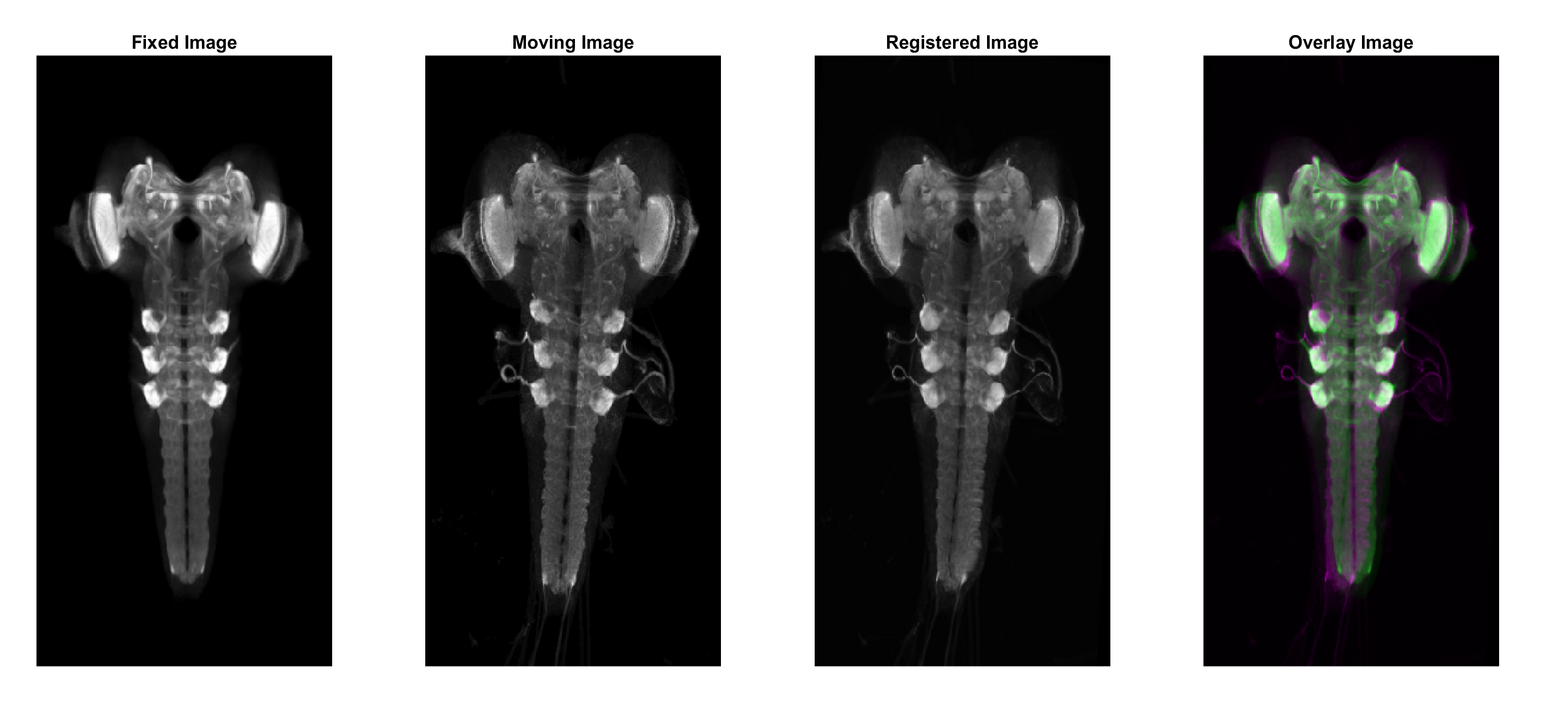
\includegraphics[width=0.9\columnwidth]{resources/chapter4/np_60H12_14E09_MB049B_020113B_scaled.tif.png}
		\caption{An example moving sample image with larger deformation where the Method 1 type of deformable registration did not produce a successful result. Four images are plotted in a row using Matlab. The first image is the fixed image against which the registration is being performed. The second image is the moving image that is being registered. The third image is the result of the registration process, and the fourth image is an overlay of the registered image and the fixed image.}
		\label{fig:method1_fail}
	\end{figure}

	 The moving image in Figure~\ref{fig:method1_fail} has large deformation at the lower tip of the Ventral Nerve Cord (VNC), and the registration process is not successful as evident (magenta region at the lower tip of VNC) in the corresponding overlay image. In contrast, the Voxelmorph method produces good results in the Figure~\ref{fig:method1_pas}. The good results produced by the Voxelmorph method in this case can be attributed to the absence of significant deformation in the moving image and the model's ability to handle smaller deformations effectively.

	\begin{figure}[h!]
		\centering
		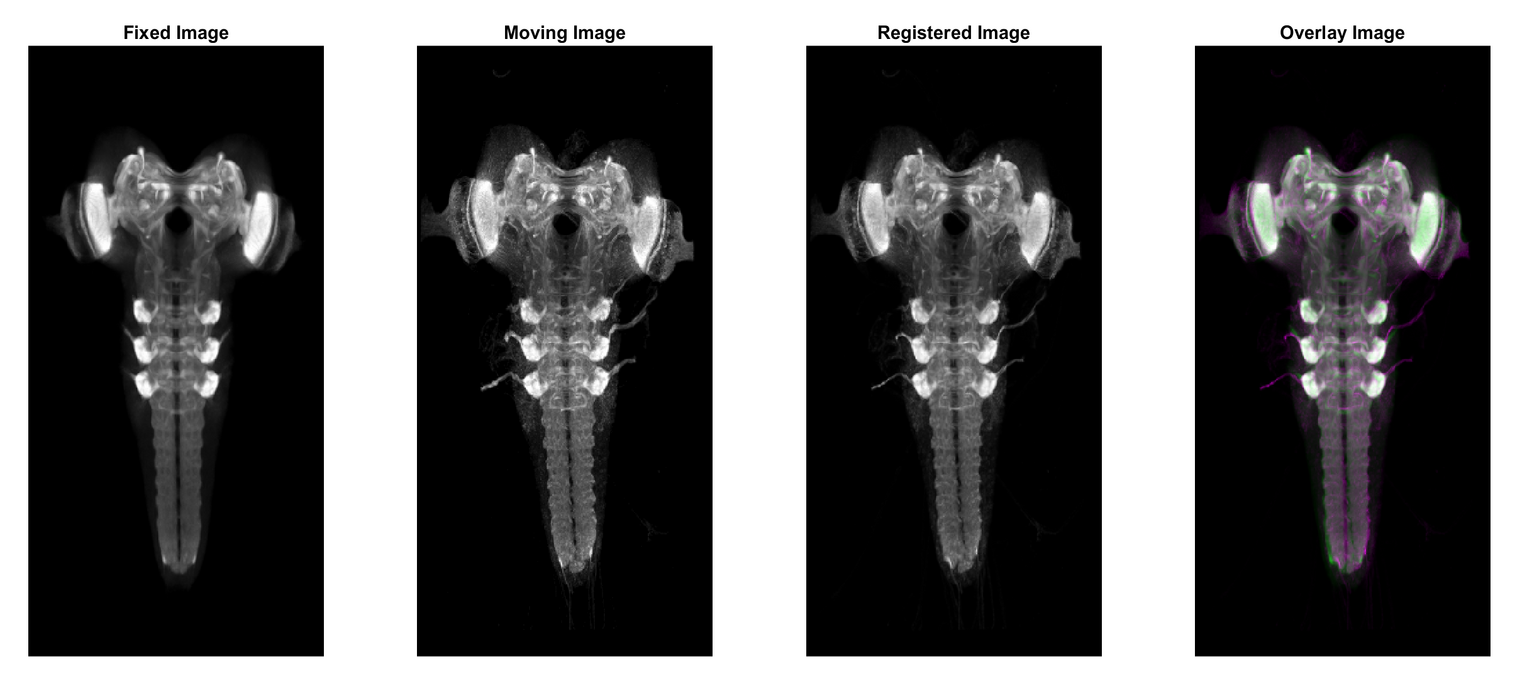
\includegraphics[width=0.9\columnwidth]{resources/chapter4/np_brain7_scaled.tif.png}
		\caption{An example moving sample image with smaller deformation where the Method 1 type of deformable registration produced a successful result. Four images are plotted in a row using Matlab. The first image is the fixed image against which the registration is being performed. The second image is the moving image that is being registered. The third image is the result of the registration process, and the fourth image is an overlay of the registered image and the fixed image.}
		\label{fig:method1_pas}
	\end{figure}
	
	\subsubsection{Motivation for Method2}
	The model clearly struggled with handling large deformations, specifically in the lower ventricular nerve chord region of the brain. In order to improve the model's performance in these cases, we provided it with additional, manually annotated information for both the moving and fixed images. This helped guide the model towards achieving better alignment, particularly when dealing with large deformations. By including this extra information in the training process, we aimed to improve the model's ability to register brain images with significant deformations.
	
	The practice of adding additional, manually annotated information for both the moving images and fixed image is referred to as Method 2. This method is explained in further detail in the following section.
	
	\subsection{Method2: Enhancing Method 1 with Novel Landmark Information.}
	As described in Section~\ref{sec:landmark_points}, in image registration, landmarks are considered to be the "Gold Standard" for determining the accuracy of the registration process. The goal is to align the fixed and moving images in such a way that the landmarks in both images matched perfectly, resulting in a landmark registration error (LRE) of zero. The LRE is the Euclidean distance between the landmarks in the registered and fixed images and to improve the accuracy of the registration, the LRE is used as an additional loss function for the network, and thus encouraging the model to learn the registration process to minimize the LRE.
	
	Biologists identified 30 points on the drosophila larva that could be used as landmarks for image registration (Figure~\ref{fig:landmark_annotations}). However, manually annotating all 30 landmarks on every training sample is time-consuming. For samples with minimal deformations, the raw Voxelmorph model [Subsection \ref{subsec:method1}] already performed well, so additional annotations are not needed. Even in cases where the Voxelmorph model did not perform well, the poor performance is only observed in specific regions, such as the tip of the Ventral Nerve Cord (VNC). Therefore, we only need annotations on samples where the raw Voxelmorph model has difficulty achieving accurate registration. To be more specific, we choose to annotate only in such samples and in such regions where we are certain that Voxelmorph would require assistance. This means that each training sample may have a different number of landmarks, including zero. To address this issue, we developed a method that can take into account of the presence of variable number of landmarks between the training samples and calculate the average landmark registration error (LRE). This allowed us to minimize the annotation effort while still obtaining good performance from the model.
	
	Incorporating landmark points as auxiliary information is a novel method that has not been used previously. The original Voxelmorph paper utilized segmentation maps to help improve registration results. With the knowledge of how Method 1 worked, the following figure \ref{fig:block_method2} will illustrate the Method 2.
	
	\begin{figure}[h!]
		\centering
		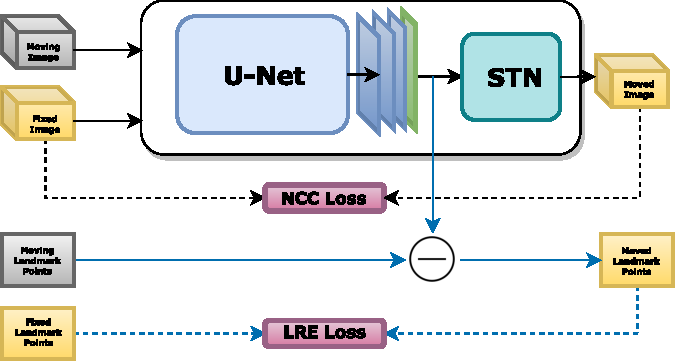
\includegraphics[width=0.6\columnwidth]{resources/chapter4/methods/Method2.pdf}
		\caption{A visual guide to training Method 2 - the raw Voxelmorph model with landmark points as auxiliary information.}
		\label{fig:block_method2}
	\end{figure}
	
	The optimization function we attempted to minimize was:
	\begin{equation}
	L_\text{combined} = L_\text{main} + L_\text{aux} \label{eqn:combined_loss}
	\end{equation}	
	
	Let's call the main loss $L_\text{main}$ and the landmark registration error $L_\text{aux}$.
	
	\textbf{Main loss}:
	\begin{equation}
	L_\text{main} = -\frac{1}{N} \sum_{i=1}^N \text{NCC}(Fixed, Moved_i) \label{eqn:main_loss}
	\end{equation}
	
	\textbf{Landmark registration error}:
	\begin{equation}
		L_\text{aux} = \frac{1}{NL} \sum_{n=1}^N \sum_{l=1}^L \sqrt{(p_l - q_{n,l})^2}
		\label{eqn:aux_loss}
	\end{equation}
	
	In this Equation~\ref{eqn:main_loss}, N is the number of moving images, and $NCC(Fixed, Moved_i)$ is the normalized cross correlation between $Fixed$ and $Moved_i$. The loss function is the negative average of the normalized cross correlation between the fixed image and each of the moving images.
	
	In this Equation~\ref{eqn:aux_loss}, N is the number of moving images, L is the number of landmarks, p\_l is the coordinates of the l-th landmark in the fixed image, and q\_{n,l} is the coordinates of the l-th landmark in the n-th moving image. The auxiliary loss is the average of the euclidean distance between the landmarks in the fixed image and the landmarks in each of the moving images.
	
	
	\subsubsection{Results}
	Using the same configurations as in Method 1, landmark points as auxiliary information was incorporated into the training. The model was retrained on the \texttt{Janelia dataset} and tested on the \texttt{Larvalign dataset}. It was found that there is an improvement in the registration accuracy with landmark points as auxiliary information.
	
	The following figures, Figure~\ref{fig:method2_fail} and Figure~\ref{fig:method2_pas}, show the results of registration using Method 2 on the same example samples used in Method 1.
	
	\begin{figure}[h!]
		\centering
		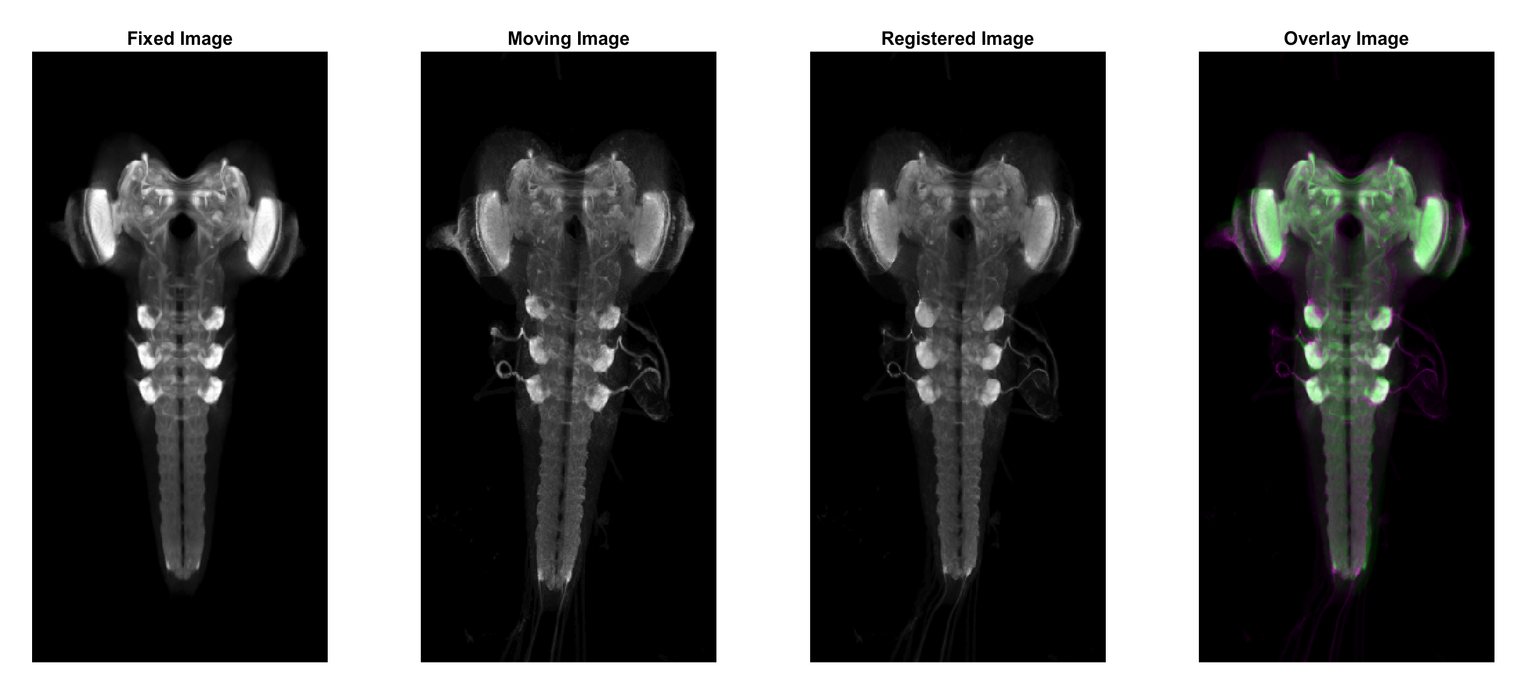
\includegraphics[width=0.9\columnwidth]{resources/chapter4/method2/np_60H12_14E09_MB049B_020113B_scaled.tif.png}
		\caption{An example moving sample image with larger deformation where the Method 2 type of deformable registration could produce a successful result when large deformation is present in contrast to Method 1. Four images are plotted in a row using Matlab. The first image is the fixed image against which the registration is being performed. The second image is the moving image that is being registered. The third image is the result of the registration process, and the fourth image is an overlay of the registered image and the fixed image.}
		\label{fig:method2_fail}
	\end{figure}
		
	Method 2 produced significantly improved registered results compared to Method 1, as can be evidenced in the two figures Figure~\ref{fig:method1_fail} and Figure~\ref{fig:method2_fail}. In Figure~\ref{fig:method1_fail}, Method 1 failed to produce satisfactory registration, particularly at the lower tip of the VNC. However, in Figure~\ref{fig:method2_fail}, it can be witnessed that with the help of landmark information, Method 2 was able to successfully register the image. The results in both figures demonstrate the efficacy of using landmark information in improving registration accuracy.

	For the moving image with little deformation like in Figure~\ref{fig:method1_pas}, the model continued to produce accurate registration results, as expected. This can be verified in the Figure~\ref{fig:method2_pas}.
	
	\begin{figure}[H]
		\centering
		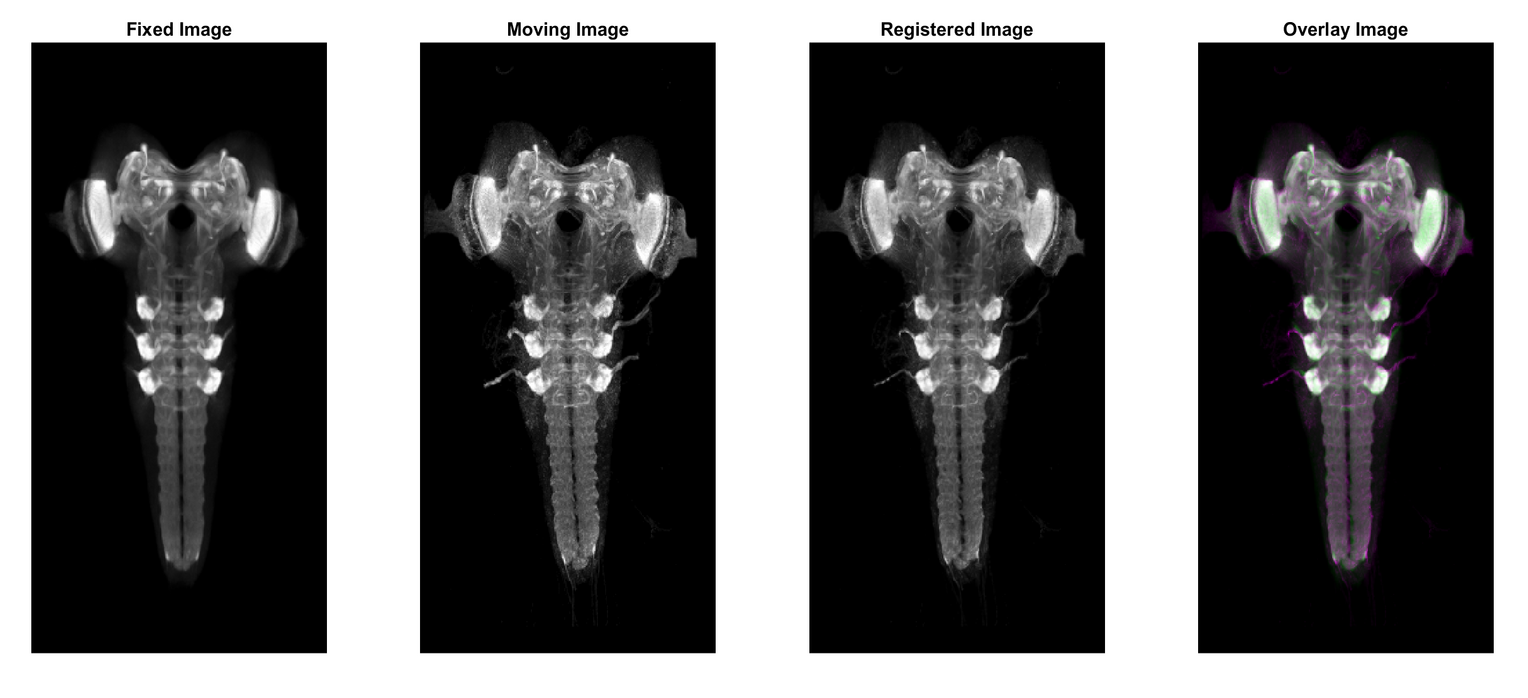
\includegraphics[width=0.9\columnwidth]{resources/chapter4/method2/np_brain7_scaled.tif.png}
		\caption{An example moving sample image with smaller deformation where the Method 2 type of deformable registration could contine to produce a successful result like Method 1. Four images are plotted in a row using Matlab. The first image is the fixed image against which the registration is being performed. The second image is the moving image that is being registered. The third image is the result of the registration process, and the fourth image is an overlay of the registered image and the fixed image.}
		\label{fig:method2_pas}
	\end{figure}
	
	While the incorporation of landmarks did improve registration accuracy, in some cases, on moving images with significant deformation, this model produced artifacts on the registered output. An example of this can be seen in the following Figure~\ref{fig:method2_artifact}.
	
	The two images in focus on the lower tip of the Ventral Nerve Cord (VNC) show the moving image before and after registration. As seen, it appears as though the structures in this area have been erased after the registration was performed.
	
	\begin{figure}[h!]
		\centering
		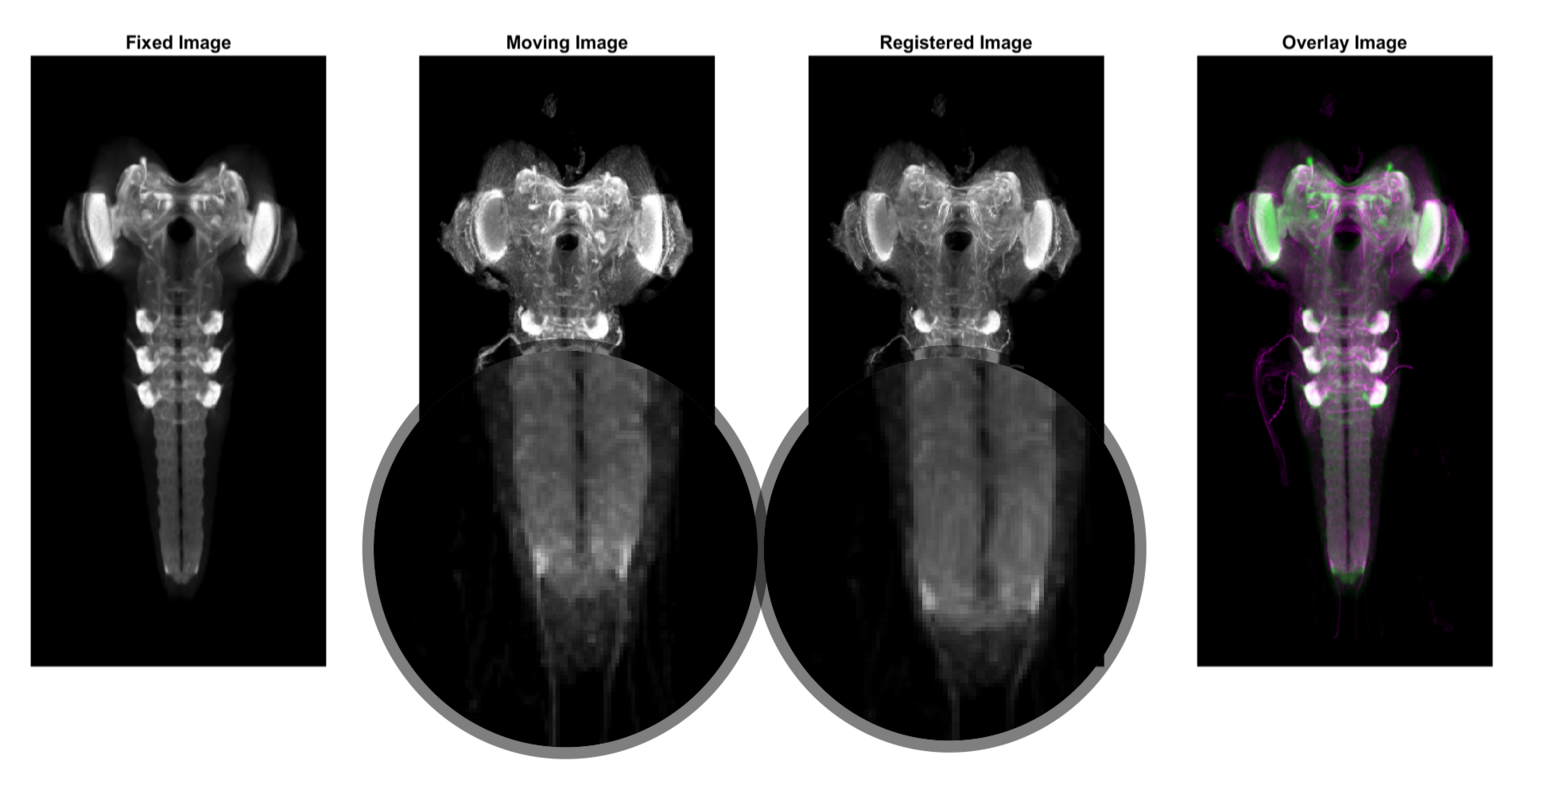
\includegraphics[width=0.9\columnwidth]{resources/chapter4/method2/np_52B07_52H01_MB262B_021713B_scaled.png}
		\caption{An example moving sample image with large deformations at the lower tip of Ventral Nerve Cord (VNC) where the Method 2 produced an artifact on the registered output. Four images are plotted in a row using Matlab. The first image is the fixed image against which the registration is being performed. The second image is the moving image that is being registered. The third image is the result of the registration process, and the fourth image is an overlay of the registered image and the fixed image.}
		\label{fig:method2_artifact}
	\end{figure}
	
	\subsubsection{Motivation for Method3}
	The artifact is commonly observed on moving images with large deformations and may be due to the model's inherent limitations in handling such large deformations. The addition of auxiliary information and loss is trying to enforce the model to achieve near perfect registration, while the model is not yet capable of doing it. This new force in play can cause the network to compromize on the qualitative features while gaining good scores in terms of error scores. To fix this problem, we need to make the model better at handling large deformations. We can also use the auxiliary information as a guide, but it should not be the main way to solve the problem.
	
	\subsection{Method3: Pyramid Gaussian Filtering and Cascaded Training.}
	Image registration is a challenging task because the optimization surface can be complex and lead to suboptimal results if the model gets stuck in one such local optima. However, literature study has shown that performing registration in a coarse-to-fine fashion can help the model escape such local optima and reach one of the better global optima. This approach has been effective in both the pre-deep learning and deep learning eras.
	
	This technique, called "pyramid registration," involves applying pyramid-style Gaussian filters and aligning images from the lowest resolution to the highest resolution. This method is effective because it ensures that the images are aligned starting with the large structures at the lowest resolutions, and then gradually aligning the finer structures as the resolution increases.
		
	Thus, the method involves processing an image at five different resolutions, and aligning the images in a coarse-to-fine manner, starting at the lowest resolution and gradually increasing the resolution at each stage. At each stage, the transformation learned in the previous stage is incorporated into the current stage in a cascaded manner. To decrease the resolution of the image, a Gaussian blur is applied using different values of $\sigma$, while keeping the width and height of the image constant. This process can be represented mathematically using the equation for Gaussian blurring.
	
	Let's say we have an input image with pixel values $I(x, y)$, and we want to apply Gaussian blurring to it using a kernel with size $n \times n$. The resulting image, $G(x, y)$, can be computed as follows:
	
	\begin{equation}\label{eqn:GaussBlur}
		G(x, y) = \frac{1}{Z} \sum_{s=-\frac{n}{2}}^{\frac{n}{2}}\sum_{t=-\frac{n}{2}}^{\frac{n}{2}}I(x+s, y+t) \cdot K(s, t)
	\end{equation}
	
	where $K(s, t)$ is the Gaussian kernel and $Z$ is a normalization factor. The Gaussian kernel is defined as:
	
	\begin{equation}
		K(s, t) = \frac{1}{2\pi \sigma^2} \exp\left(-\frac{s^2+t^2}{2\sigma^2}\right)
	\end{equation}
	
	Here, $\sigma$ is a parameter that determines the amount of blur applied to the image. A larger value of $\sigma$ results in more blur. The size of the kernel, $n$, is usually chosen to be an odd number such as 3, 5, or 7. We start by processing the image at the lowest resolution, where the value of $\sigma$ is set to 4. In subsequent stages, we progressively increase the resolution of the image by decreasing the value of $\sigma$ to 2, 1, 0.5, and finally to 0, which is the original resolution of the image.
	The process is illustrated in the Figure \ref{fig:block_method3}.
	
    \begin{figure}[h!]
		\centering
		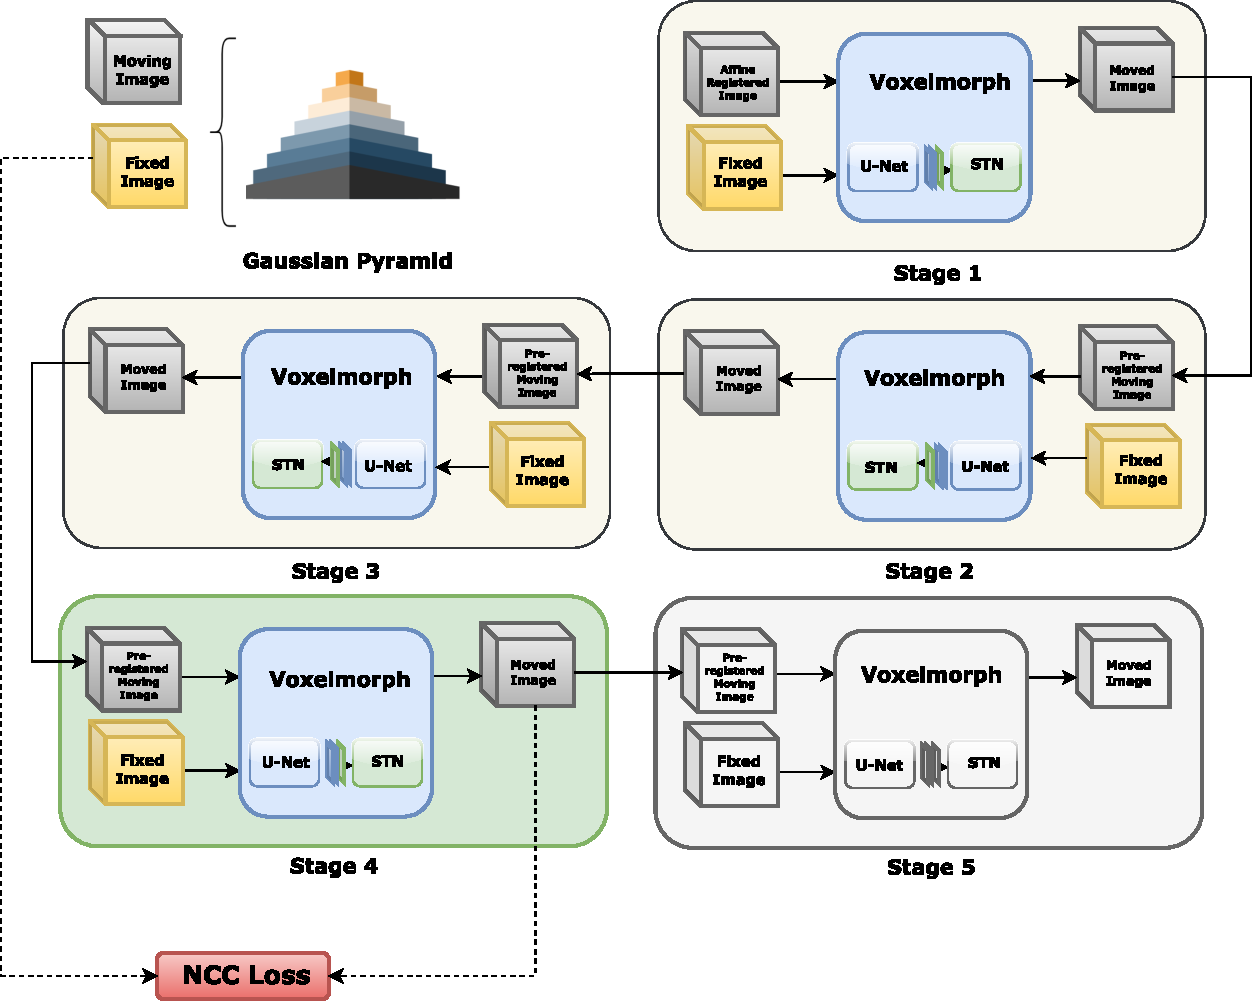
\includegraphics[width=\columnwidth]{resources/chapter4/methods/Method3.pdf}
		\caption{This process involves 5 stages, each of which is trained independently. At any given time, only one stage (colored green) is being trained, while the other stages (colored white or gray) are either frozen or not in use. The input for the current stage (colored green) is selected from a list of Gaussian filtered images and passes through the previous stages (colored white) to be pre-registered before being used for training. The stages located after the current stage (colored gray) are not utilized during this training process.}
		\label{fig:block_method3}
	\end{figure}

	This method for image registration uses multiple Voxelmorph model without auxiliary information and with the same configurations connected in a cascaded fashion. Both the moving and fixed images were pre-processed with Gaussian blurring using different sigma values for each stage.
	
	\subsubsection{Stages}
	For each stage, the appropriate inputs (fixed image and moving image) are chosen from the Gaussian Pyramid. To help explain the process, we will refer to the inputs for each stage as input1 through input5, with input1 representing the input images for stage 1 (blurred with sigma = 4), input2 representing the input images for stage 2 (blurred with sigma = 2), and so on. The final input, input5, consists of the original, unmodified images. We will also refer to the models for each stage as model1 through model5. The optimization function (Normalized Cross Correlation) used in all these stage aims to maximize the similarity between the moved and fixed images.
	
	\begin{equation}
		L = -\frac{1}{N} \sum_{i=1}^N \text{NCC}(Fixed, Moved_i)
	\end{equation}
	
	where:
	\begin{itemize}
		\item $\text{L}$ is the loss function.
		\item $N$ is the number of moving images.
		\item $\mathbf{Moved}_i$ is the $i$th moved image.
		\item $\mathbf{Fixed}$ is the fixed image.
		\item $NCC(\mathbf{Fixed}, \mathbf{Moved}_i)$ is the normalized cross correlation between the $i$th moved image and the fixed image.
	\end{itemize}
	
	\paragraph{Stage 1}
	In stage 1, the model is trained using input images that has been pre-processed with Gaussian blurring using sigma = 4. The predicted deformation field from this model is used to transform the input image, creating a version called the "moved image." This moved image is then compared to the fixed image, which has also been pre-processed with Gaussian blurring using sigma = 4. All other stages are not used and will be grayed out.
	
	\paragraph{Stage 2}
	In stage 2, the model is trained using input images that have been pre-processed with a Gaussian blur of sigma = 2. After completing the training for stage 1, the trained model parameters are frozen (white) and used for coarse alignment of input2 images. These coarsely aligned input2 images are then used to train stage 2 to predict a deformation field, which is applied to the input image using a spatial transformer network to produce a transformed moving image called the "moved" image. The moved image is compared to the fixed image, which has been pre-processed with a Gaussian blur of sigma = 2, to compute the similarity value. The other stages are unused.
	
	\paragraph{Stage 3, 4 and 5}
	The aforementioned steps are repeated iteratively for all subsequent stages, using the previously trained and frozen models to incorporate the learned transformation and coarsely align the images for the current training stage. This process follows a coarse-to-fine approach, meaning that the transformation is initially learned at a coarser resolution and then successively refined at finer resolutions.
	
	\subsubsection{Results}
	There were no artifacts introduced when registering the moving sample using this model, as can be seen in the Figure~\ref{fig:method3_artifact}. This was confirmed by comparing the results to the reference image in Figure~\ref{fig:method2_artifact}
	
	Method 3 performed better than the previous two methods in terms of registering the moving samples with large and smaller deformations, as shown in Figure~\ref{fig:method3_pas} and Figure~\ref{fig:method3_fail}. However, there was room for improvement at the lower tip of the Ventral Nerve Cord (VNC) where the nerve entry points can be aligned more accurately.
	
	\begin{figure}[h!]
		\centering
		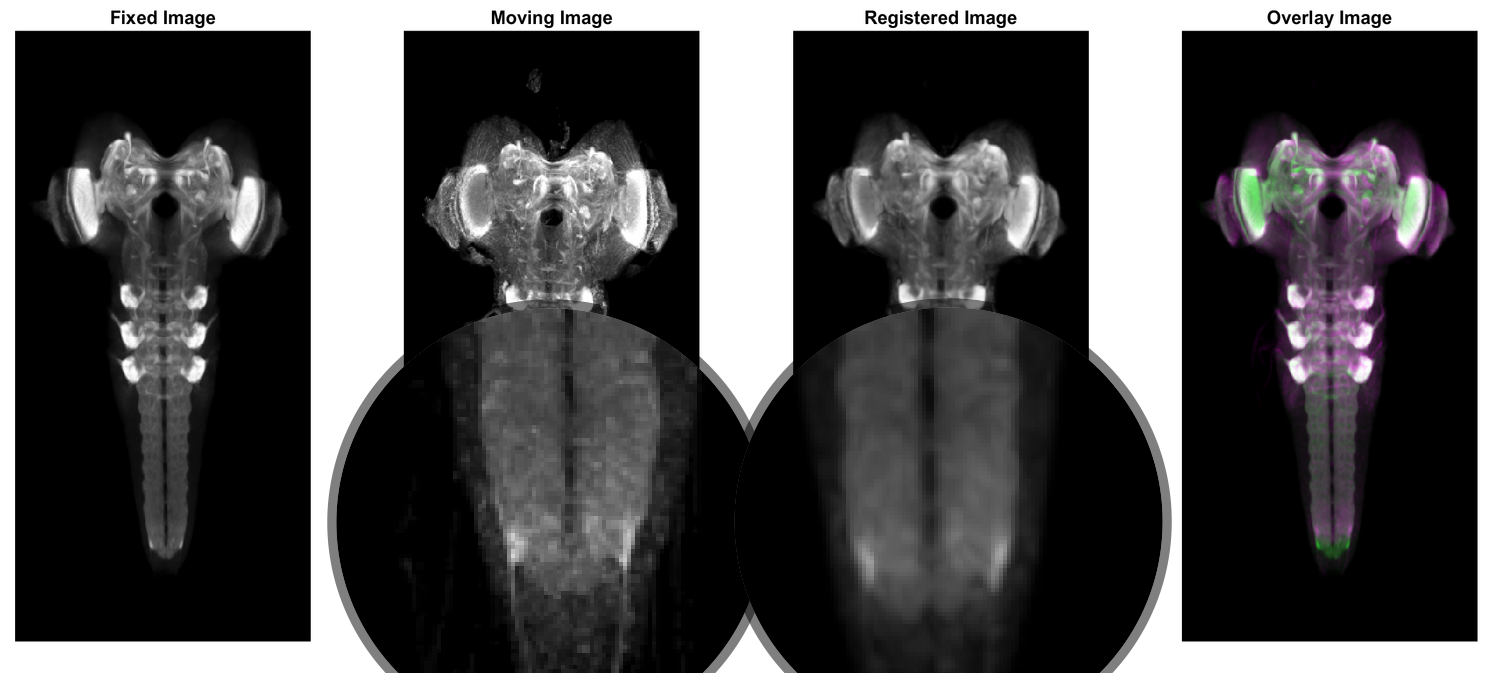
\includegraphics[width=0.9\columnwidth]{resources/chapter4/method3/compare/np_52B07_52H01_MB262B_021713B_scaled.png}
		\caption{An example moving sample image with large deformations at the lower tip of Ventral Nerve Cord (VNC) where the Method 3 did not produce an artifact on the registered output. Four images are plotted in a row using Matlab. The first image is the fixed image against which the registration is being performed. The second image is the moving image that is being registered. The third image is the result of the registration process, and the fourth image is an overlay of the registered image and the fixed image.}
		\label{fig:method3_artifact}
	\end{figure}
	
	\begin{figure}[h!]
		\centering
		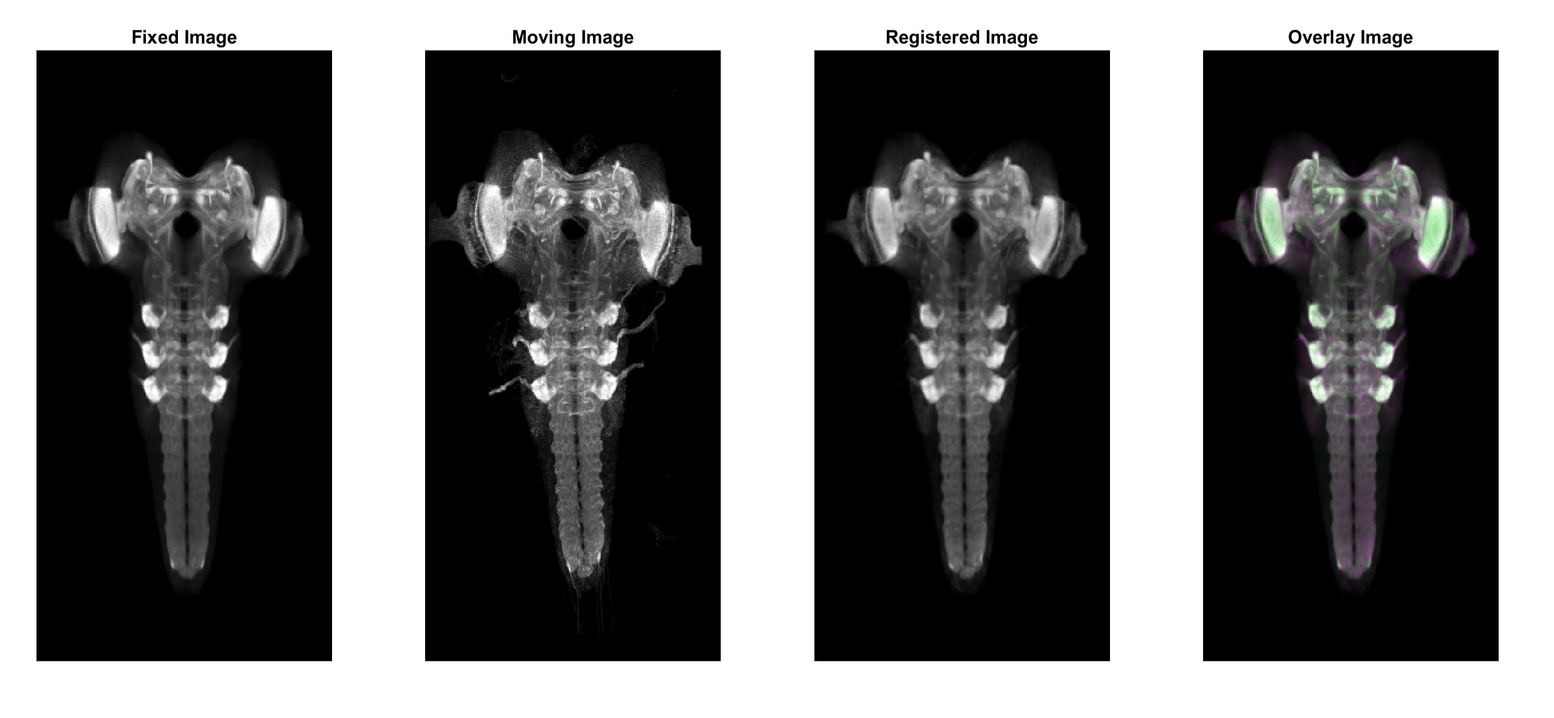
\includegraphics[width=0.9\columnwidth]{resources/chapter4/method3/compare/np_brain7_scaled.tif.png}
		\caption{An example moving sample image with smaller deformation where the Method 3 type of deformable registration could continue to produce a successful result like Method 1 and Method 2. Four images are plotted in a row using Matlab. The first image is the fixed image against which the registration is being performed. The second image is the moving image that is being registered. The third image is the result of the registration process, and the fourth image is an overlay of the registered image and the fixed image.}
		\label{fig:method3_pas}
	\end{figure}

	\begin{figure}[h!]
		\centering
		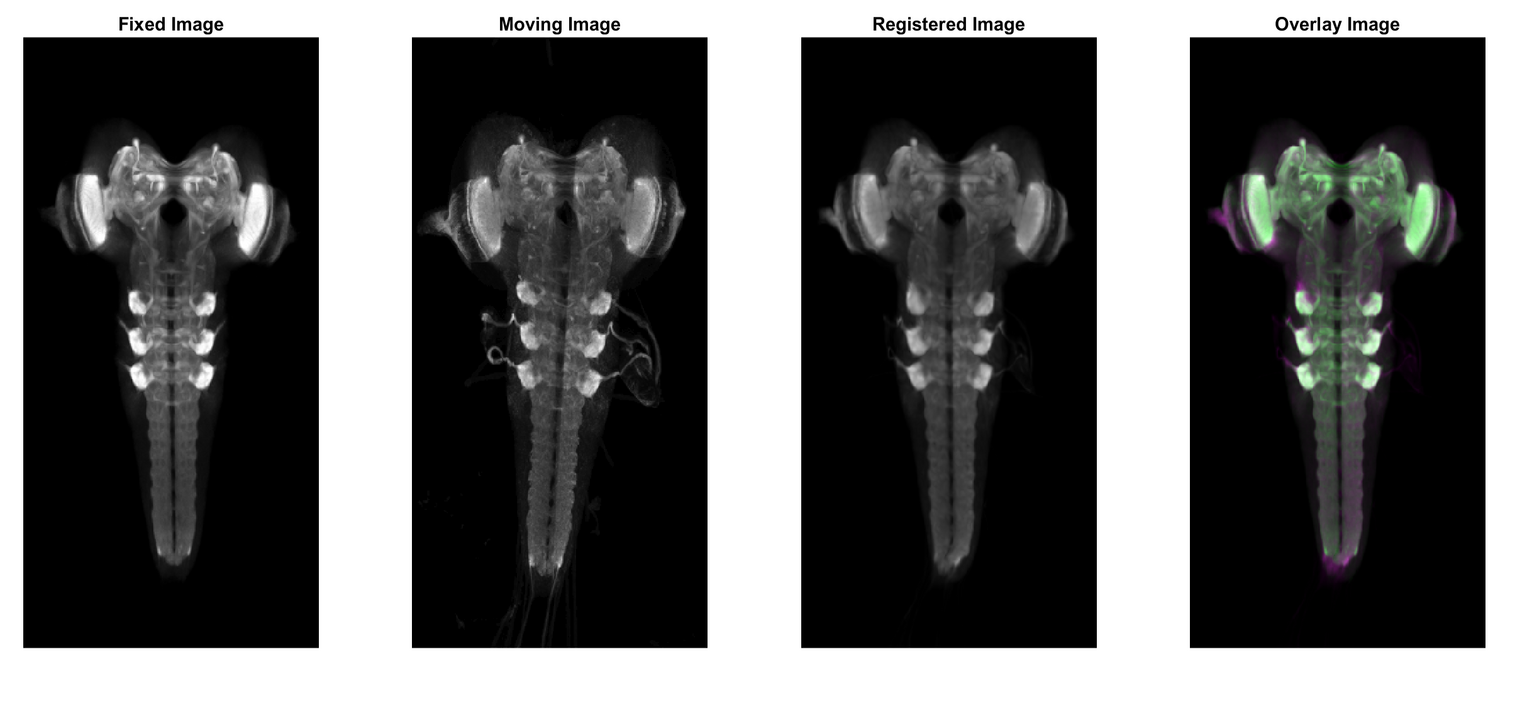
\includegraphics[width=0.9\columnwidth]{resources/chapter4/method3/compare/np_60H12_14E09_MB049B_020113B_scaled.tif.png}
		\caption{An example moving sample image with larger deformation where the Method 3 type of deformable registration could produce a successful result when large deformation is present in contrast to Method 1. Four images are plotted in a row using Matlab. The first image is the fixed image against which the registration is being performed. The second image is the moving image that is being registered. The third image is the result of the registration process, and the fourth image is an overlay of the registered image and the fixed image.}
		\label{fig:method3_fail}
	\end{figure}
	
	The following Figure~\ref{fig:method3_cascade} demonstrate the output of the registered moving image as it is propogated through each stage of the cascade. The corrections are applied in a coarse to fine manner, with the transformation becoming more precise at progressively higher resolutions as the sample progresses through these stages.
	
	\begin{figure}[h!]
		\centering
		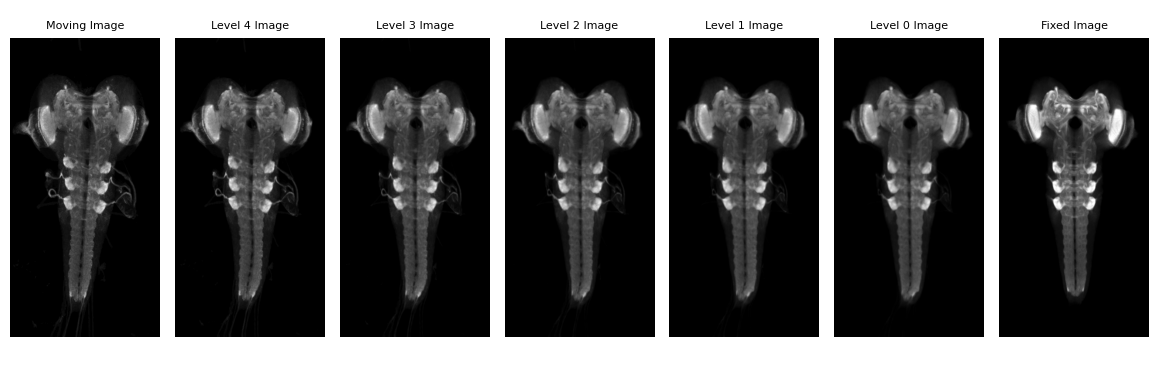
\includegraphics[width=\columnwidth]{resources/chapter4/method3/np_60H12_14E09_MB049B_020113B_scaled.png}
		\caption{Registration output through a series of cascaded stages performed in a coarse-to-fine manner.}
		\label{fig:method3_cascade}
	\end{figure}
	
	\subsubsection{Motivation for Method4}
	This method was able to handle large deformations more effectively than the raw Voxelmorph model used in Method 1 and at the same time not producing any artifacts. The results demonstrated this. While the results were satisfactory, there was a clear potential for further improvement at the lower end of the Ventral Nerve Cord by incorporating landmark point information during training, as seen in the results of Method 2. Further experiments will be conducted to assess the benefits of adding this additional information in the next method.
	
	\subsection{Method4: Enhancing Method 3 with Novel Landmark Information.}
	In Method 2, the use of landmark information was found to improve performance. However, incorporating this information into Method 4 is not straightforward because the input for each stage consists of different pre-aligned image samples, meaning that the landmarks annotated in one stage cannot be used in later stages due to the pre-alignment process moving them to different positions. Manually re-annotating the landmarks for each stage is impractical, especially if there are many stages or a large number of images. To solve this problem, we developed a method that allows us to incorporate the landmark information at all stages without requiring manual re-annotation. Our approach is based on the fact that the input images for each stage are the same except for the different levels of Gaussian blurring applied. This means that the initial annotations made on any of these images can still be used at later stages if we can propagate the landmarks to their new positions using the predicted deformation field, similar to the pre-alignment process for images.
	
	This is again a novel method that has been introduced in this theis work. These moved landmarks, called "pseudo-annotated" landmarks, may not be as accurate as manually annotated landmarks, but they were precise enough to work with the blurred images in the earlier stages where the structures were not clear to require precise manual annotation.
	
	The Equation~\ref{eq:ldm_prop} states that the new position of the landmark is obtained by subtracting the deformation field at that position from the old position of the landmark.
	
	\begin{equation}\label{eq:ldm_prop}
		l_n^{new} = l_n^{old} - d_n
	\end{equation}
	
	where:
	
	$l_n^{new}$ is the new position of the landmark in image $n$. $l_n^{old}$ is the old position of the landmark in image $n$. $d_n$ is the deformation field for image $n$ at the position of the landmark.
	
	Method 4 combines aspects of Method 2 and Method 3 in an attempt to take advantage of the strengths of both approaches. Like Method 3, it involves processing an image at five different resolutions and aligning the images in a coarse-to-fine manner, starting at the lowest resolution and gradually increasing it at each stage. The transformation learned in the previous stage is incorporated into the current stage in a cascaded manner. To decrease the resolution of the image, a Gaussian blur is applied using different values of sigma, while the width and height of the image remain constant. This process is represented mathematically using equation \ref{eqn:GaussBlur}. And like Method 2, we use the auxiliary information in the form of landmark points to help neural network train in the right direction.
	
	\begin{figure}[h!]
		\centering
		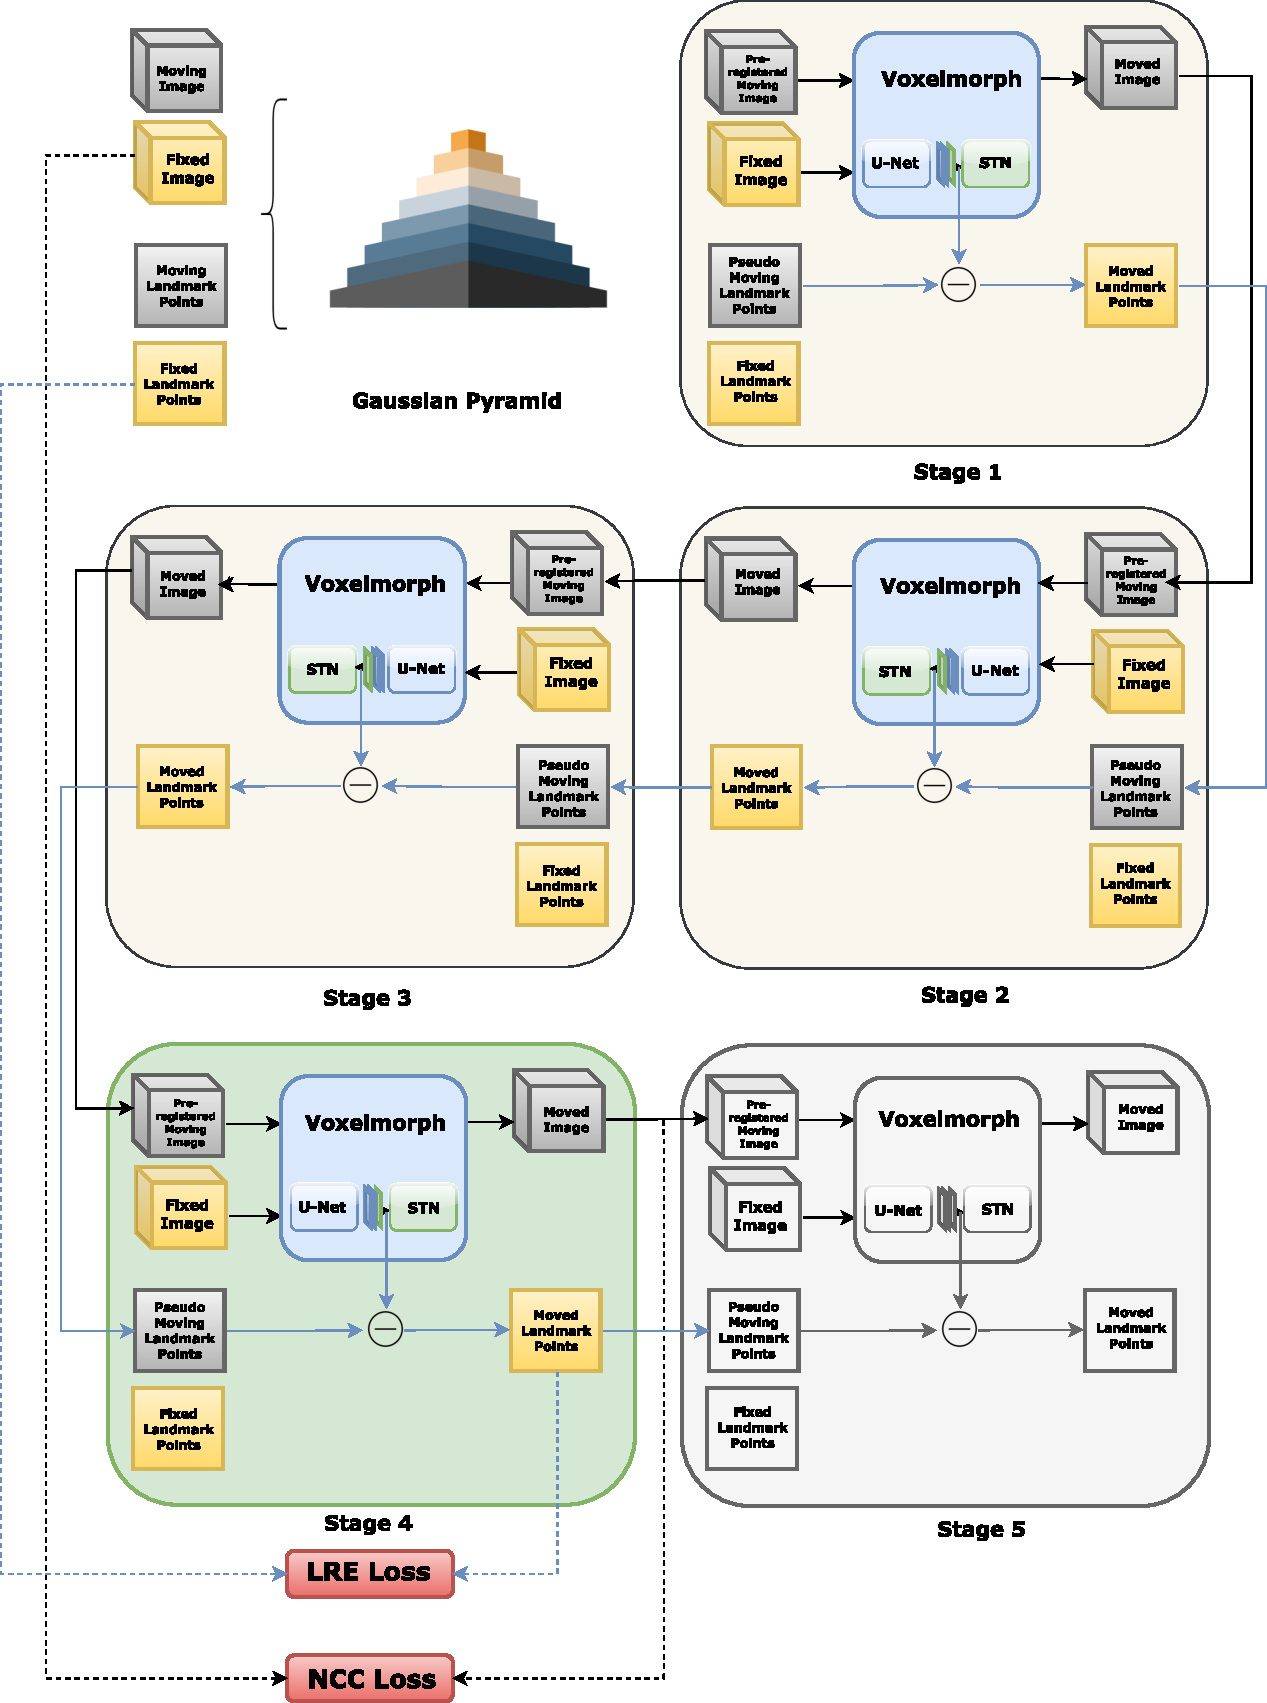
\includegraphics[width=\columnwidth]{resources/chapter4/methods/Method4.pdf}
		\caption{This process consists of 5 stages, each of which is trained separately. Only one stage (indicated by the color green) is being trained at a given time, while the other stages (colored white or gray) are either inactive or not being used. The input for the current stage (colored green) is selected from a list of Gaussian filtered images and passes through the previous stages (colored white) to be pre-registered before being used for training. The stages that come after the current stage (colored gray) are not used during this training process. In addition to the images, the landmark points are also used to calculate the landmark registration error (LRE) at each stage during training.}
		\label{fig:block_method4}
	\end{figure}
	
	\subsubsection{Stages}
	For each stage, the appropriate inputs (fixed image and moving image) are chosen from the Gaussian Pyramid. To help explain the process, we will refer to the inputs for each stage as input1 through input5, with input1 representing the input images for stage 1 (blurred with sigma = 4), input2 representing the input images for stage 2 (blurred with sigma = 2), and so on. The final input, input5, consists of the original, unmodified images. We will also refer to the models for each stage as model1 through model5. The optimization function (Normalized Cross Correlation) used in all these stage aims to maximize the similarity between the moved and fixed images. Additionally, the model is also evaluated based on the landmark registration error to guide the learning process.
	
	Therefore, the optimization function attempted to minimize was:
	\begin{equation}\label{eq:aux_loss_combined}
		L_\text{combined} = L_\text{main} + L_\text{aux}
	\end{equation}
	
	Let us call the main loss $L_\text{main}$ and the landmark registration error $L_\text{aux}$.
	
	\textbf{Main loss:}
	\begin{equation}\label{eq:aux_loss_main}
		L_\text{main} = -\frac{1}{N} \sum_{i=1}^N \text{NCC}(Fixed, Moved_i)
	\end{equation}
	
	\textbf{Landmark registration error:}
	\begin{equation}\label{eq:aux_loss_aux}
		L_\text{aux} = \frac{1}{NL} \sum_{n=1}^N \sum_{l=1}^L \sqrt{(p_l - q_{n,l})^2}
	\end{equation}
	
	In this Equation~\ref{eq:aux_loss_main}, N is the number of moving images, and $NCC(Fixed, Moved_i)$ is the normalized cross correlation between $Fixed$ and $Moved_i$. The loss function is the negative average of the normalized cross correlation between the fixed image and each of the moving images.
	
	In this Equation~\ref{eq:aux_loss_aux}, N is the number of moving images, L is the number of landmarks, p\_l is the coordinates of the l-th landmark in the fixed image, and q\_{n,l} is the coordinates of the l-th landmark in the n-th moving image. The auxiliary loss is the average of the euclidean distance between the landmarks in the fixed image and the landmarks in each of the moving images.
	
    The whole process is described in the Figure~\ref{fig:block_method4}
	
	\paragraph{Stage 1}
	In stage 1, the model is trained using input images that has been pre-processed with Gaussian blurring using sigma = 4. The predicted deformation field from this model is used to transform the input image, creating a version called the "moved image." This moved image is then compared to the fixed image, which has also been pre-processed with Gaussian blurring using sigma = 4. All other stages are not used and will be grayed out.

	\paragraph{Stage 2}
	In stage 2 of this process, the model is trained on input images that have been blurred using a Gaussian blur with a sigma value of 2. The trained model from stage 1 is then frozen and used to coarsely align the input2 images. These aligned images are used to train stage 2 to predict a deformation field, which is applied to the input image using a spatial transformer network to create a transformed image called the "moved" image. The moved image is compared to a fixed image, which has also been blurred using a Gaussian blur with a sigma value of 2, to calculate a similarity value. The later stages are not used in this process. Stage 2 uses "pseudo-annotated" landmarks, which are obtained by propagating manually annotated landmarks from the previous stage using the deformation field predicted by model1.
	
	\begin{equation}\label{eq:pseudoldm}
		landmark_{stage2,m,n} = landmark_{stage1,m,n} - deformation\_field_{stage1,m,n}
	\end{equation}
	
	Here, 
	\begin{itemize}
		\item "$landmark_{stage2,m,n}$" is the landmark point for stage 2 at pixel m for image n.
		\item "$landmark_{stage1,m,n}$" is the landmark point for stage 1 at pixel m for image n.
		\item "$deformation\_field_{stage1,m,n}$" is the deformation field from stage 1 at pixel m for image n.    
	\end{itemize}
	
	This Equation~\ref{eq:pseudoldm} is valid for all values of m such that m is a landmark point for an image in stage 1, and for all values of n such that n belongs to N, where N is the number of images in stage 2.
	
	\paragraph{Stage 3 and 4}
	The aforementioned steps are repeated iteratively for all subsequent stages, using the previously trained and frozen models to incorporate the learned transformation and coarsely align the images for the current training stage. This process follows a coarse-to-fine approach, meaning that the transformation is initially learned at a coarser resolution and then successively refined at finer resolutions.
	
	The following pseudo code demonstrates how landmarks are propagated from stage 1 to stage 's' by utilizing the deformation model at each stage.
	
	\begin{lstlisting}[language=Python]
	# N: The number of landmark lists.
	# M: The number of landmark points in each landmark list.
	# S: The number of stages.
	for n in range(N):
	# n: The index of the current landmark list.
		for m in range(M):
		# m: The index of the current landmark point.
			for s in range(S):
			# s: The index of the current stage.
				# deformation_field: The deformation field for the current stage.
				deformation_field = find_deformation_field(s)
				# old_landmark_point: The old landmark point for the current landmark point
				# and stage.
				# new_landmark_point: The new landmark point for the current landmark point
				# and stage, which is calculated by subtracting the deformation field from
				# the old landmark point.
				new_landmark_point = old_landmark_point - deformation_field
				# Update the landmark point with the new value.
				update_landmark_point(new_landmark_point)
	\end{lstlisting}
	
	\paragraph{Stage 5: The last stage}
	The initial approach for aligning images in the final stage of the process involved using software to propagate the previously identified landmarks. However, it was ultimately decided to manually annotate the landmarks again in order to improve accuracy. This is because the images used in this stage are the original, unmodified ones, and using landmarks that were generated with the help of the previous, pre-aligned images may not be accurate enough. By manually annotating the landmarks, the final registration can be more precise.
	
	\subsubsection{Results}
	The Figure~\ref{fig:method4_combine} consists of 3 moving image samples in 3 rows. Each column represents the output of the corresponding movie image through different stages through the cascaded network. This figure is representative of the output from Method 4.
	
	\begin{figure}[H]
		\centering
		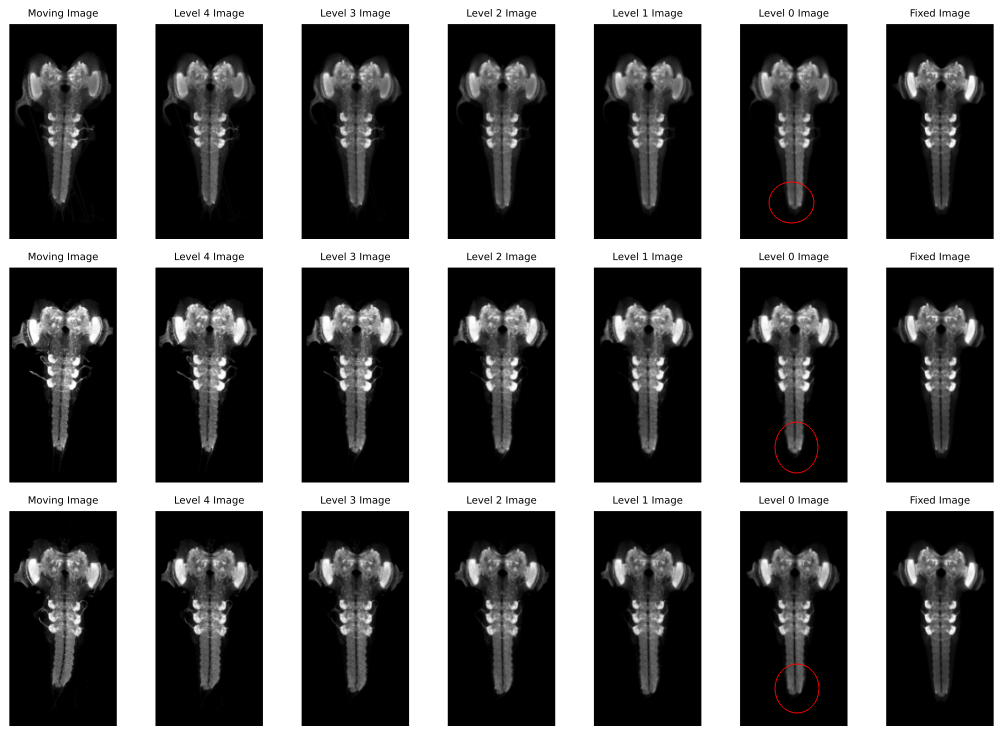
\includegraphics[width=0.6\columnwidth]{resources/chapter4/method4/ldm/registered_images.png}
		\caption{Coarse-to-fine registration using landmark information.}
		\label{fig:method4_combine}
	\end{figure}

	Similarly, the Figure~\ref{fig:method3_combine} consists of same 3 moving image samples in 3 respective rows. Each column, again, represents the output of the corresponding movie image through different stages through the cascaded network. This figure is representative of the output from Method 3.
	
	\begin{figure}[H]
		\centering
		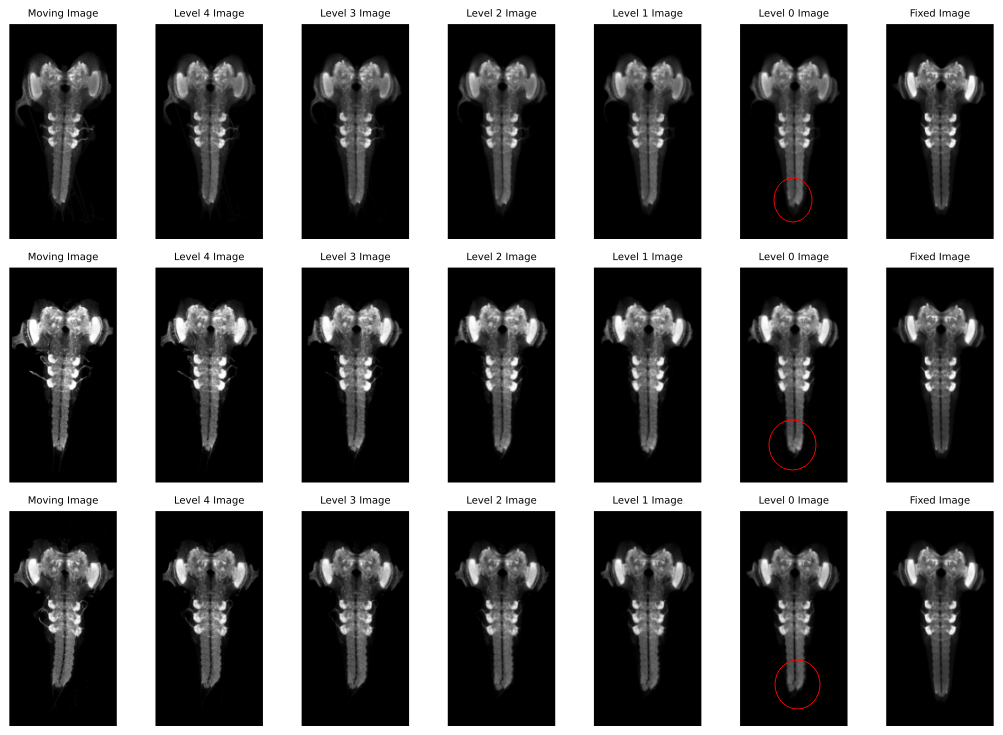
\includegraphics[width=0.6\columnwidth]{resources/chapter4/method4/vanilla/registered_images.png}
		\caption{Coarse-to-fine registration without using landmark information.}
		\label{fig:method3_combine}
	\end{figure}
	
	
	Comparing the figures Figure~\ref{fig:method4_combine} and Figure~\ref{fig:method3_combine}, it is evident that adding landmark points at the lower tip of the Ventral Nerve Cord has resulted in better registration accuracy for Method 4 than for Method 3.	

	\chapter{Results}
	In the following sections, we will evaluate the performance of our proposed approaches and compare them to the "\emph{larvalign}" approach using the "\texttt{Larvalign dataset}". We will use the metrics introduced in the sections \ref{sec:loss_metric} and \ref{sec:quality} to assess the effectiveness of these approaches.
	
	\section{Assessment on \emph{larvalign} method}
	Before presenting the results of the approaches we have developed in this thesis, we will first present the results of the "\emph{larvalign}" method. This will provide a baseline or benchmark against which we can compare the performance of our approaches.
	
	\subsection{Quantitative Assessment Metric}
	The table \ref{table:quant_larvalign} presents the results of three different metrics used to quantitatively assess the performance of the image registration on the medium quality images in "\texttt{Larvalign Dataset}":
	\begin{enumerate}
		\item The "VI" or "ventricular nerve entry error indicator" measures the error in the alignment of the ventricular nerve cord region in the images.
		\item The "TI" or "thoracic nerve entry error indicator" measures the error in the alignment of the thoracic nerve entry regions in the images.
		\item The "MMI" or "Mattes Mutual Information" measures the overall similarity between the fixed image and the registered image.
	\end{enumerate}
	
	The average score obtained for all the images in the \texttt{Larvalign dataset} is captured in the below table \ref{table:quant_larvalign_avg}
	
	\begin{table}[H]
		\centering
		\begin{tabular}{|l|l|l|l|}
			\hline
			 & \textbf{MMI} & \textbf{VI} & \textbf{TI} \\ \hline
			Average Score & 76.88 & 84 & 71 \\ \hline
		\end{tabular}
		\caption{The average Mattes Mutual Information, VI Error Indicator, and TI Error Indicator for the all the images in \texttt{Larvalign Dataset} for \emph{larvalign} method.}
		\label{table:quant_larvalign_avg}
	\end{table}

	\begin{table}[!h]
		\centering
		\begin{tabular}{|l|l|l|l|}
			\hline
			\textbf{Scan} & \textbf{MMI} & \textbf{VI} & \textbf{TI} \\ \hline
			\textbf{np\_GL\_09B11\_AE\_01\_012410A\_scaled.tif} & 67 & 84 & 58 \\ 
			\textbf{np\_GL\_10A07\_AE\_01\_011511B\_scaled.tif} & 73 & 92 & 71 \\ 
			\textbf{np\_GL\_24B09\_AE\_01\_102709B\_scaled.tif} & 33 & 5 & 65 \\ 
			\textbf{np\_GL\_24H06\_AE\_01\_062508A\_scaled.tif} & 26 & 0 & 48 \\ 
			\textbf{np\_GL\_31B04\_AE\_01\_031911B\_scaled.tif} & 61 & 88 & 57 \\ 
			\textbf{np\_GL\_39A12\_AE\_01\_051609B\_scaled.tif} & 81 & 96 & 66 \\ 
			\textbf{np\_GL\_39H11\_AE\_01\_080409B\_scaled.tif} & 48 & 41 & 62 \\ 
			\textbf{np\_GL\_43A11\_AE\_01\_101609B\_scaled.tif} & 61 & 68 & 61 \\ 
			\textbf{np\_GL\_43A12\_AE\_01\_101210B\_scaled.tif} & 72 & 84 & 68 \\ 
			\textbf{np\_GL\_47C10\_AE\_01\_061509A\_scaled.tif} & 64 & 69 & 66 \\ 
			\textbf{np\_GL\_49C01\_AE\_01\_111710A\_scaled.tif} & 66 & 88 & 53 \\ 
			\textbf{np\_GL\_53A06\_AE\_01\_081209A\_scaled.tif} & 38 & 15 & 55 \\ 
			\textbf{np\_GL\_53H01\_AE\_01\_021611A\_scaled.tif} & 60 & 64 & 56 \\ 
			\textbf{np\_GL\_58E05\_AE\_01\_082709B\_scaled.tif} & 75 & 92 & 79 \\ 
			\textbf{np\_GL\_60A07\_AE\_01\_091509A\_scaled.tif} & 48 & 24 & 60 \\ 
			\textbf{np\_GL\_60F09\_AE\_01\_012010A\_scaled.tif} & 59 & 72 & 68 \\ 
			\textbf{np\_GL\_62A03\_AD\_01\_020610A\_scaled.tif} & 56 & 76 & 63 \\ 
			\textbf{np\_GL\_68B03\_AE\_01\_110408B\_scaled.tif} & 71 & 63 & 65 \\ 
			\textbf{np\_GL\_73B11\_AE\_01\_121309B\_scaled.tif} & 71 & 75 & 58 \\ 
			\textbf{np\_GL\_79B07\_AE\_01\_100110B\_scaled.tif} & 61 & 85 & 60 \\ 
			\textbf{np\_GL\_85B08\_AE\_01\_081210A\_scaled.tif} & 59 & 68 & 55 \\ 
			\textbf{np\_GL\_89B10\_AE\_01\_090410A\_scaled.tif} & 57 & 62 & 62 \\ 
			\textbf{np\_GL\_93A08\_AE\_01\_071110B\_scaled.tif} & 67 & 75 & 61 \\ 
			\textbf{np\_GL\_93F05\_AE\_01\_090310A\_scaled.tif} & 55 & 74 & 70 \\ 
			\textbf{np\_GL\_96A08\_AD\_01\_031911B\_scaled.tif} & 68 & 96 & 70 \\ \hline
		\end{tabular}
		\caption{Mattes Mutual Information, VI Error Indicator, and TI Error Indicator for the medium quality images in \texttt{Larvalign Dataset} for \emph{larvalign} method.}
		\label{table:quant_larvalign}
	\end{table}
	
	In addition to these, LRE, or landmark registration error, that measures the overall accuracy of the alignment of specific landmarks in the images was also computed for the medium quality images registered by \emph{larvalign} in \texttt{Larvalign Dataset} and is represented in the table \ref{table:lre_larvalign}. The average mean and standard deviation for the LRE measure on the medium quality images is given in this below table \ref{table:avg_lre_larvalign}
	
	\begin{table}[H]
		\centering
		\begin{tabular}{|l|l|l|}
			\hline
			\textbf{} & \textbf{Mean LRE} & \textbf{Std LRE} \\ \hline
			\textbf{Average score} & 2.10 & 1.02 \\ \hline
		\end{tabular}
		\caption{The average mean and standard deviation for the LRE measured on medium quality images in Larvalign dataset.}
		\label{table:avg_lre_larvalign}
	\end{table}
	
	\begin{table}[!h]
		\centering
		\begin{tabular}{|l|c|c|}
			\hline
			\textbf{Landmark Points} & \textbf{Mean LRE} & \textbf{Std LRE} \\ \hline
			\textbf{left thoracic nerve entry T2} & 0.91 & 0.59 \\ 
			\textbf{right MB vertical medial lobe connection} & 0.91 & 0.77 \\ 
			\textbf{right A7 nerve entry} & 3.05 & 1.21 \\ 
			\textbf{right tip of vertical lobe} & 0.74 & 0.53 \\ 
			\textbf{right basal brain neuropil border posterior} & 4.12 & 1.66 \\ 
			\textbf{right thoracic nerve entry T1} & 1.61 & 0.68 \\ 
			\textbf{Left MB vertical medial lobe connection} & 1.07 & 0.61 \\ 
			\textbf{right upper peduncle} & 1.26 & 0.66 \\ 
			\textbf{left thoracic nerve entry T1} & 1.65 & 0.68 \\ 
			\textbf{right antennal nerve} & 2.01 & 1.02 \\ 
			\textbf{left A8 nerve entry} & 2.97 & 0.96 \\ 
			\textbf{right A8 nerve entry} & 2.92 & 0.97 \\ 
			\textbf{end of ventral nerve cord} & 1.46 & 0.96 \\ 
			\textbf{left upper most anterior nerve entry} & 3.84 & 1.91 \\ 
			\textbf{left basal brain neuropil border posterior} & 4.19 & 1.52 \\ 
			\textbf{left thoracic nerve entry T3} & 1.14 & 0.79 \\ 
			\textbf{right thoracic nerve entry T2} & 0.94 & 0.53 \\ 
			\textbf{anterior upper commisure} & 1.6 & 1.12 \\ 
			\textbf{center SEZ neuropil fusion} & 2.75 & 1.36 \\ 
			\textbf{left tip of vertical lobe} & 0.91 & 0.63 \\ 
			\textbf{left antennal nerve} & 1.95 & 1.33 \\ 
			\textbf{right anterior LON nerve} & 1.68 & 0.71 \\ 
			\textbf{posterior upper commisure} & 2.59 & 1.2 \\ 
			\textbf{right upper most anterior nerve entry} & 3.94 & 2.72 \\ 
			\textbf{left A7 nerve entry} & 2.96 & 1.3 \\ 
			\textbf{right A6 nerve entry} & 3.0 & 1.01 \\ 
			\textbf{left upper peduncle} & 1.16 & 0.74 \\ 
			\textbf{left A6 nerve entry} & 3.1 & 0.93 \\ 
			\textbf{left anterior LON nerve} & 1.51 & 0.73 \\ 
			\textbf{right thoracic nerve entry T3} & 1.17 & 0.77 \\ \hline
		\end{tabular}
		\caption{The mean and standard deviation in landmark registration error recorded across all the medium quality images in \texttt{Larvalign Dataset} for \emph{larvalign} method.}
		\label{table:lre_larvalign}
	\end{table}
	
	\newpage
	
	\chapter{Discussion}
	The goal of this chapter is to provide a clear and concise summary of the key findings of the research, and to interpret and discuss their significance in relation to the research question of whether deep learning is a fast and robust method for image registration compared to the traditional way of performing image registration.
	\newpage
	
	\chapter{Conclusion}
	
	% bibiliography
	\newpage
	\bibliographystyle{ieeetr}
	\bibliography{./references}
\end{document}